\section{Simulating the LOB}


\subsection{Queuing Model}\label{ch:queue_model}
Here, I will describe the queuing model used in this thesis to simulate the LOB. It is based on the one developed by \cite{A6} but with several important modifications. I again represent the LOB as a $2K$-dimensional vector $X(t) = (q_{-K}(t), … q_{-1}(t), q_1(t), … , q_K(t))$ with the center corresponding to the reference price. Events at each position $k$ are either positive or negative with the magnitude distributed exponentially with means $\mu^+_k$ and $\mu^-_k$ respectively. That is, if a positive event occurs at time $t$ with size $e$, set $q(t) \leftarrow q(t) + e$, and if a negative event occurs at time $t$ with size $e$, set $q(t) \leftarrow (q(t) - e)^+$ where $b^+ = 0$ if $b < 0$ and $b$ otherwise (so as to keep the queue size non negative). An exception occurs when a negative order occurs at the best bid or ask. I assume it is a market order and the size is larger than the volume, fill the leftover with the next best prices. I estimate $\mu^+_k$ and $\mu^-_k$ as the $AES$ for positive and negative arrivals. Arrivals of events are jointly distributed as a multivariate Poisson process. There are $4K$ such processes, with positive and negative arrivals for $2K$ positions. The marginal arrival process is a Poisson process with positive and negative arrivals having mean rates $\lambda^+_k$ and $\lambda^-_k$ respectively. I simulate arrivals in time periods of length $b$. Let $N_{k+}(b)$ be the number of positive arrivals at position $k$ ($N_{k-}(b)$ for negative arrivals) during a time period of length $b$. Then, the arrivals have a $4K\times4K$ correlation matrix $\sigma$ where $\sigma_{i+j+}$ is the $corr(N_{i+}(b), N_{j+}(b))$ (same for negative arrivals).

Here, I will highlight the differences between this model and the queue-reactive model developed by \cite{A6} and explain the reasons for the modifications. First, the size of positive and negative events are not just the $AES$, but rather is a continuous random variable. This is because the event sizes that I found have considerable variation. I find in subsection \ref{ch:AES} that an exponential distribution reasonably fits the distribution of event sizes. Although it may not fit the data completely, this part of the model is the easiest to adjust.

Second, I do not vary the rate of arrival as the size of the queue changes. This is because I did not find a substantial change in rate as the queue size changed, and the queue size varied widely (sometimes several dozens multiplies of the AES) and I did not have enough data points to estimate the rate at some sizes. It also simplifies the model greatly.

Third, I model the arrival processes as a multivariate Poisson process instead of independent Poisson processes. In subsection \ref{ch:poisson}, I verify the claim that the arrival rates at each position reasonably follow a Poisson process. However, I find in subsection \ref{ch:correlations} that these processes are significantly correlated.

\subsection{Building An Abbreviated Order Book}
Although I maintain the full order book after each update, the queuing model only contains the first $K$ prices on the bid and ask side closest to the reference price. I therefore only estimate parameters for these positions. Usually, the reference price is the midpoint between the best bid and best ask price. However, if the best bid and ask are an even distance apart, I add or subtract 0.5 to make it closest to the previous reference price. I then restart the process of recording data.

Often in the data set, several orders of the same magnitude, sign, and inter-arrival time occur in quick succession. This is likely a trader who has split up a larger trade for whatever reason. As it should represent one trade, I combine orders that occur in quick succession (defined as occurring less than 0.01 seconds after the last) if they are at the same position and sign. See listing \ref{data-processing-code} for the code written to process the data.

\subsection{Average Event Size Estimate}\label{ch:AES}
In this section, I first examine whether the event sizes can reasonably fitted with exponential distribution with rate equal to the $AES$. 

\begin{figure}
\centering
\caption{Event Sizes Compared to Exponential Distribution (4 Positions Closest to Reference Price)}
\begin{tabular}{cc}
\hline
\subf{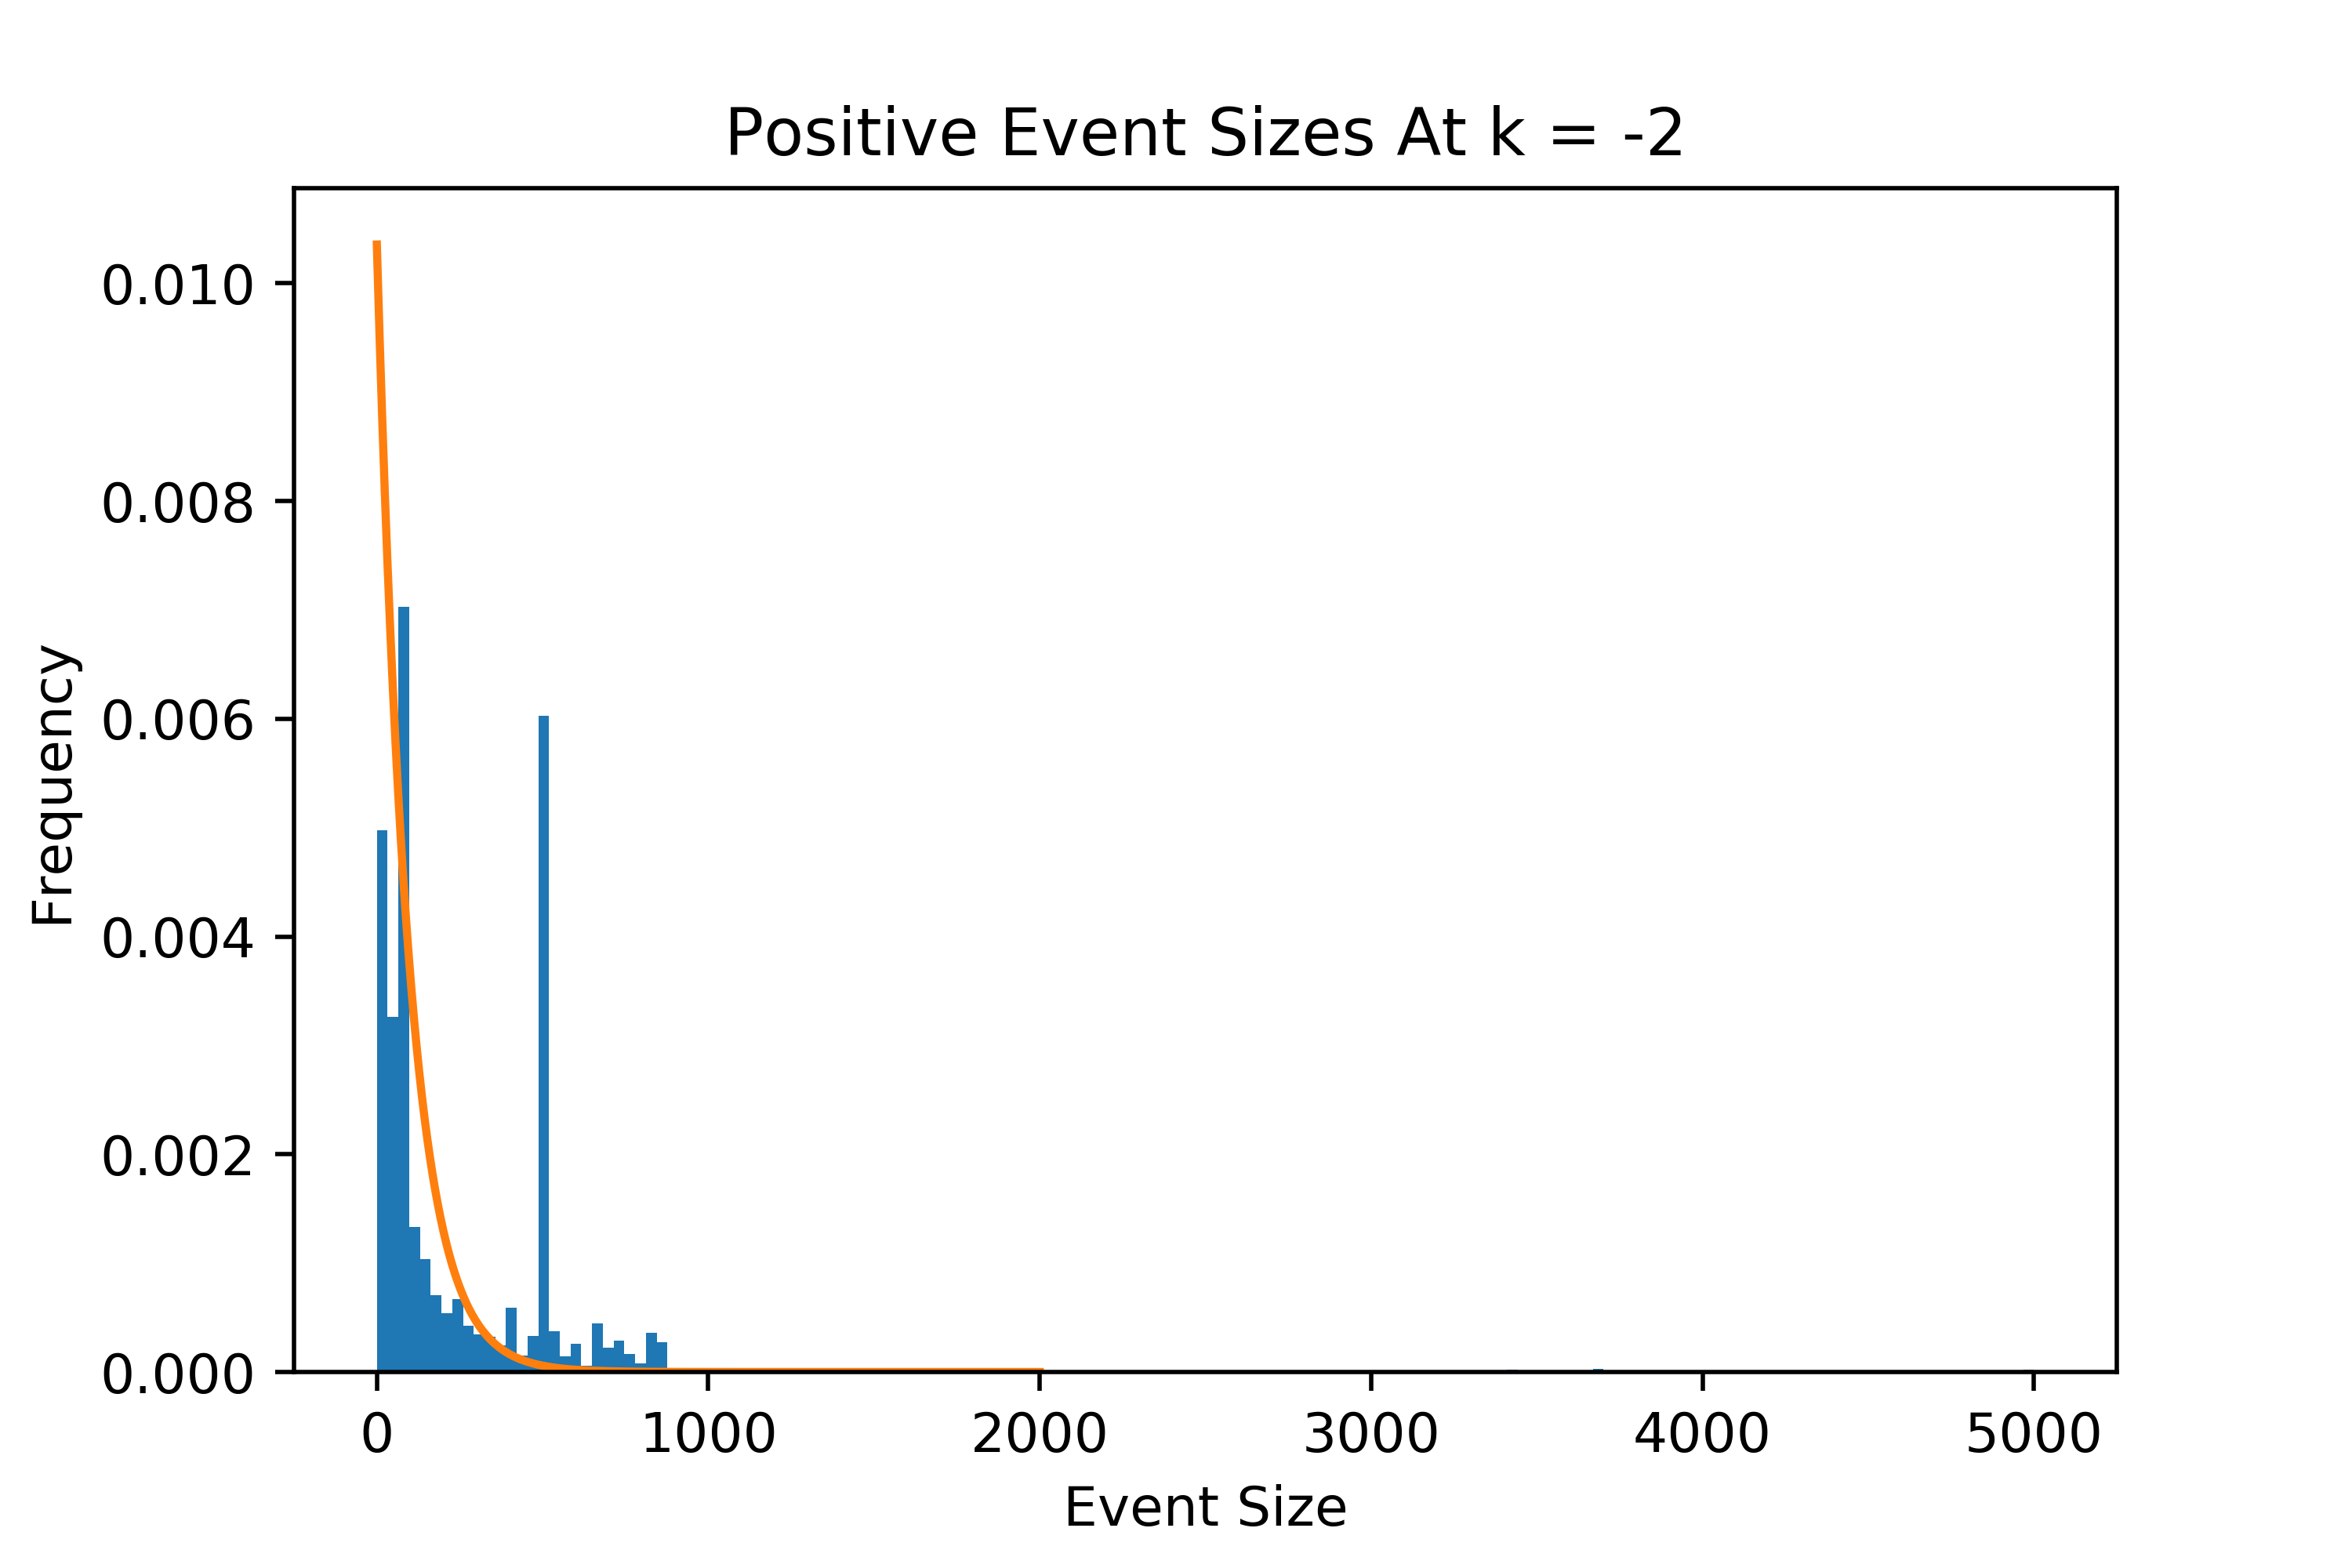
\includegraphics[width=60mm]{Figures/pos_-2.png}}
{}
&
\subf{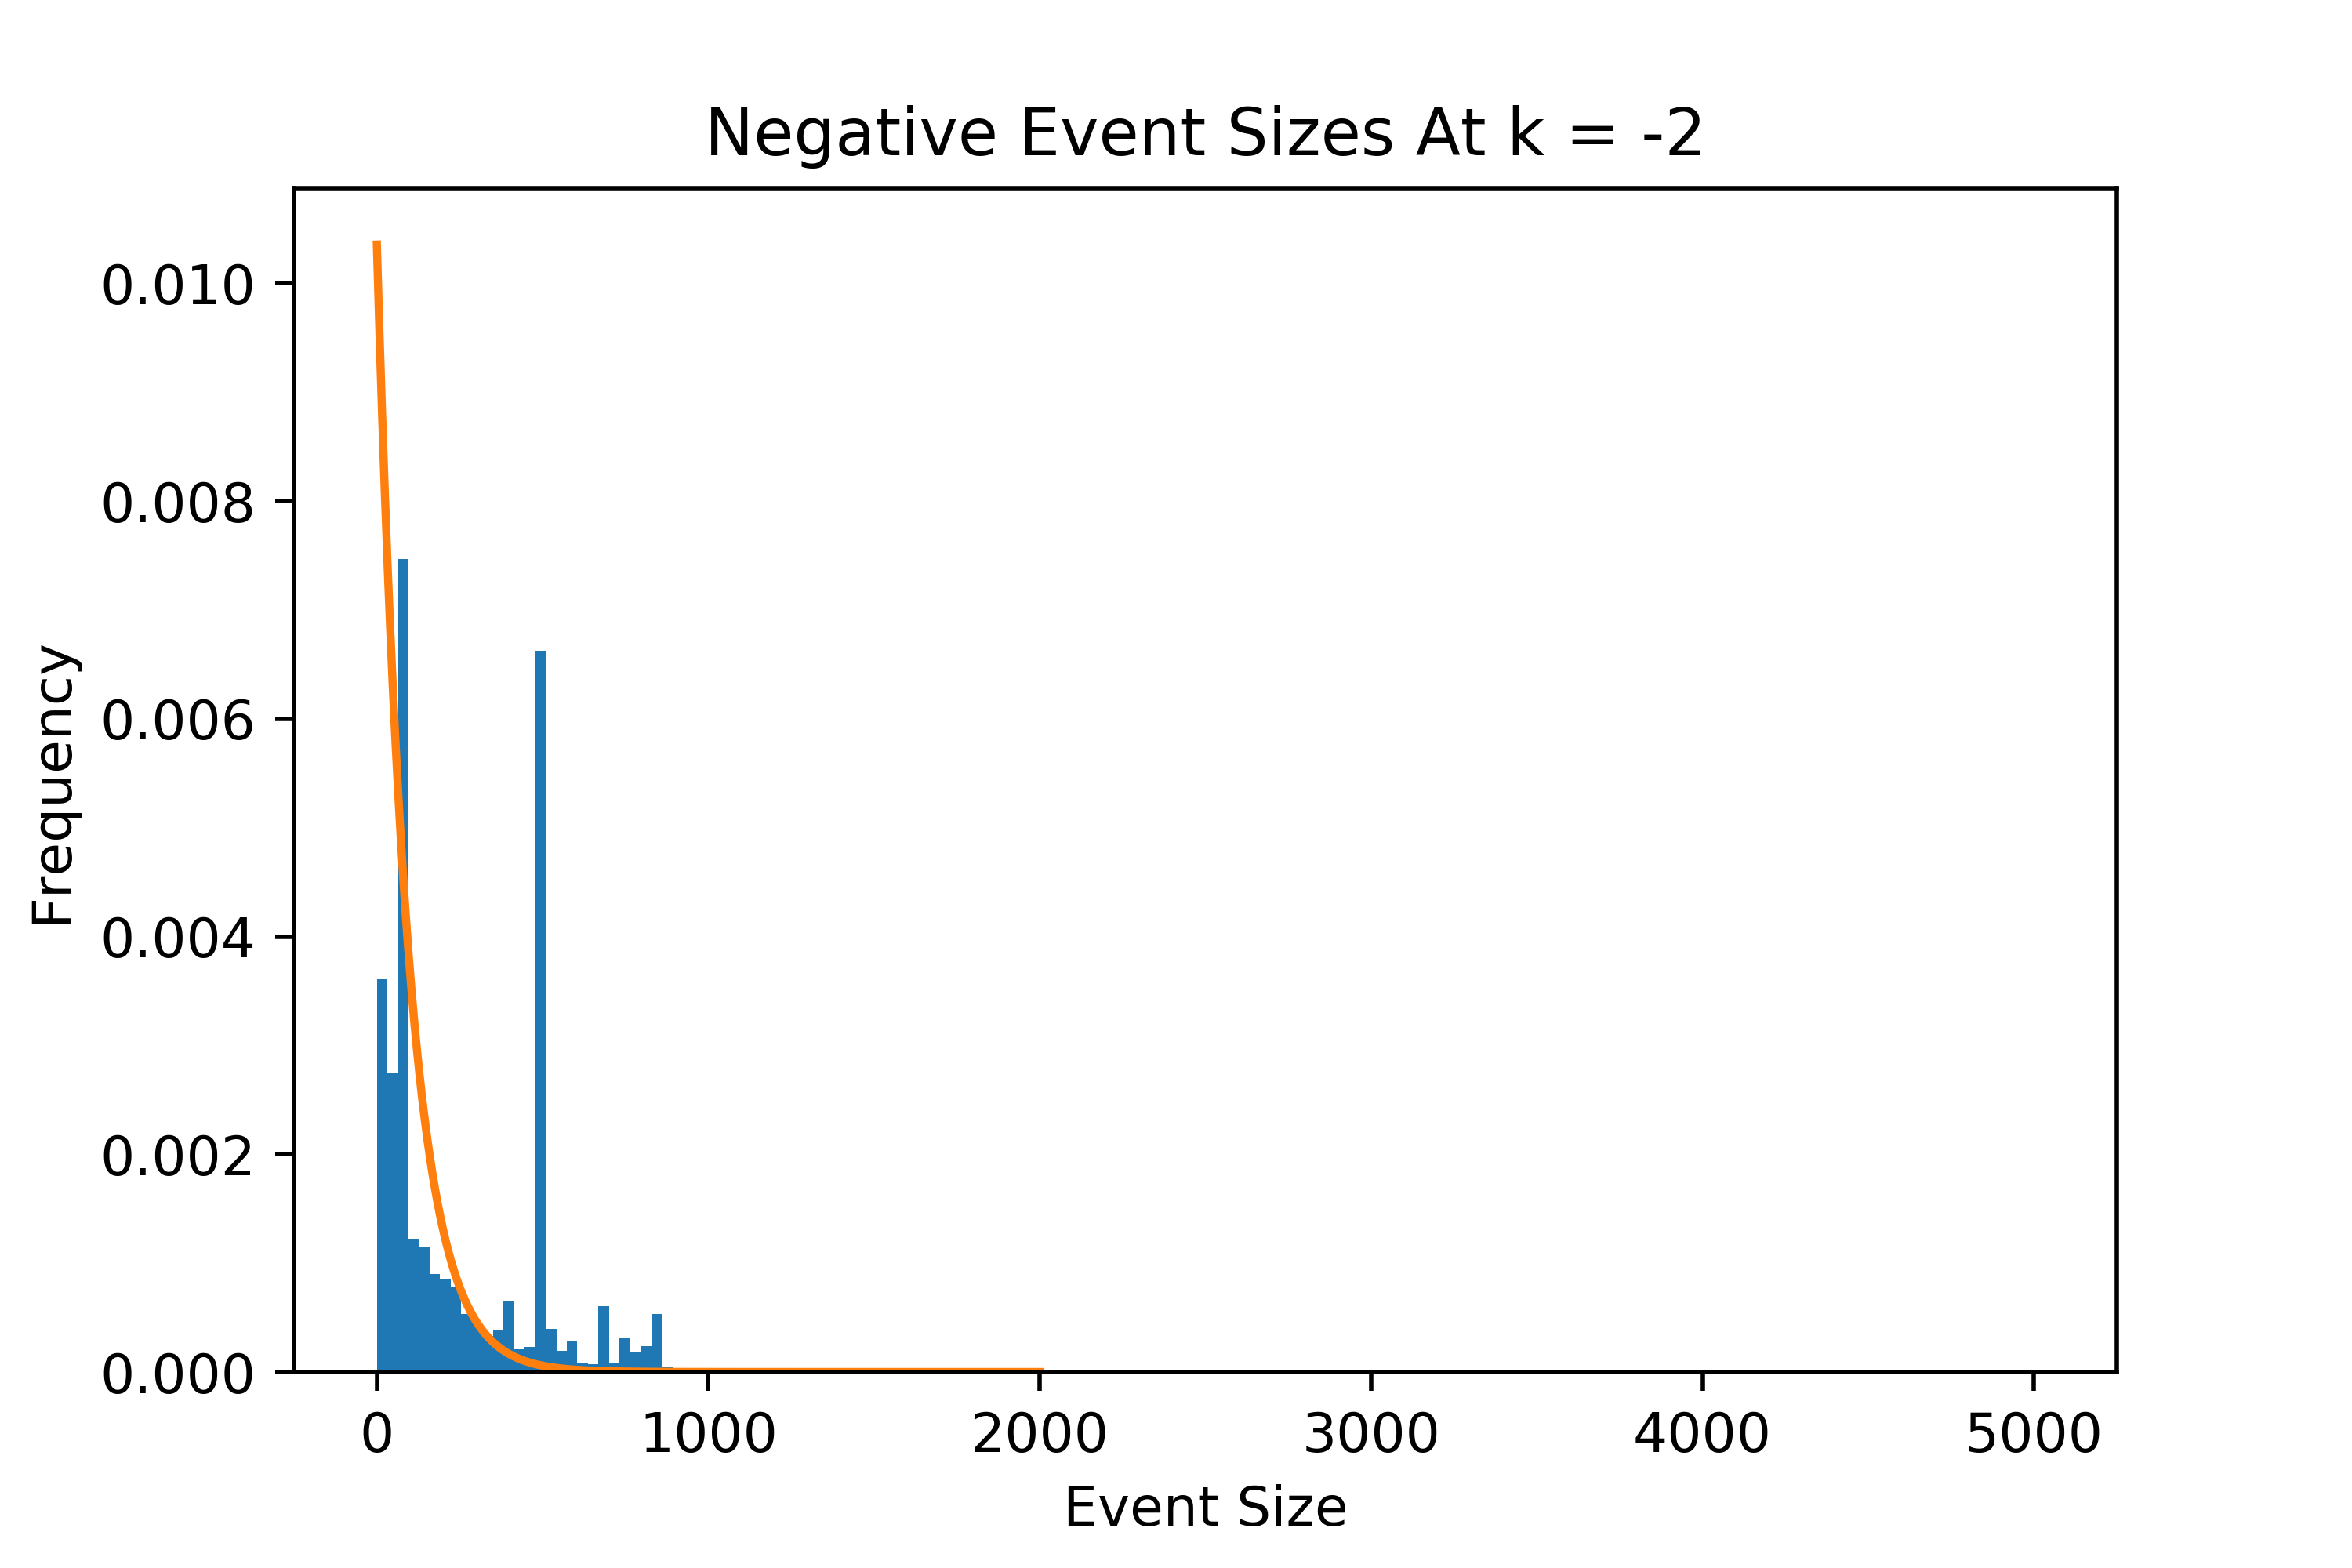
\includegraphics[width=60mm]{Figures/neg_-2.png}}
{}
\\
\subf{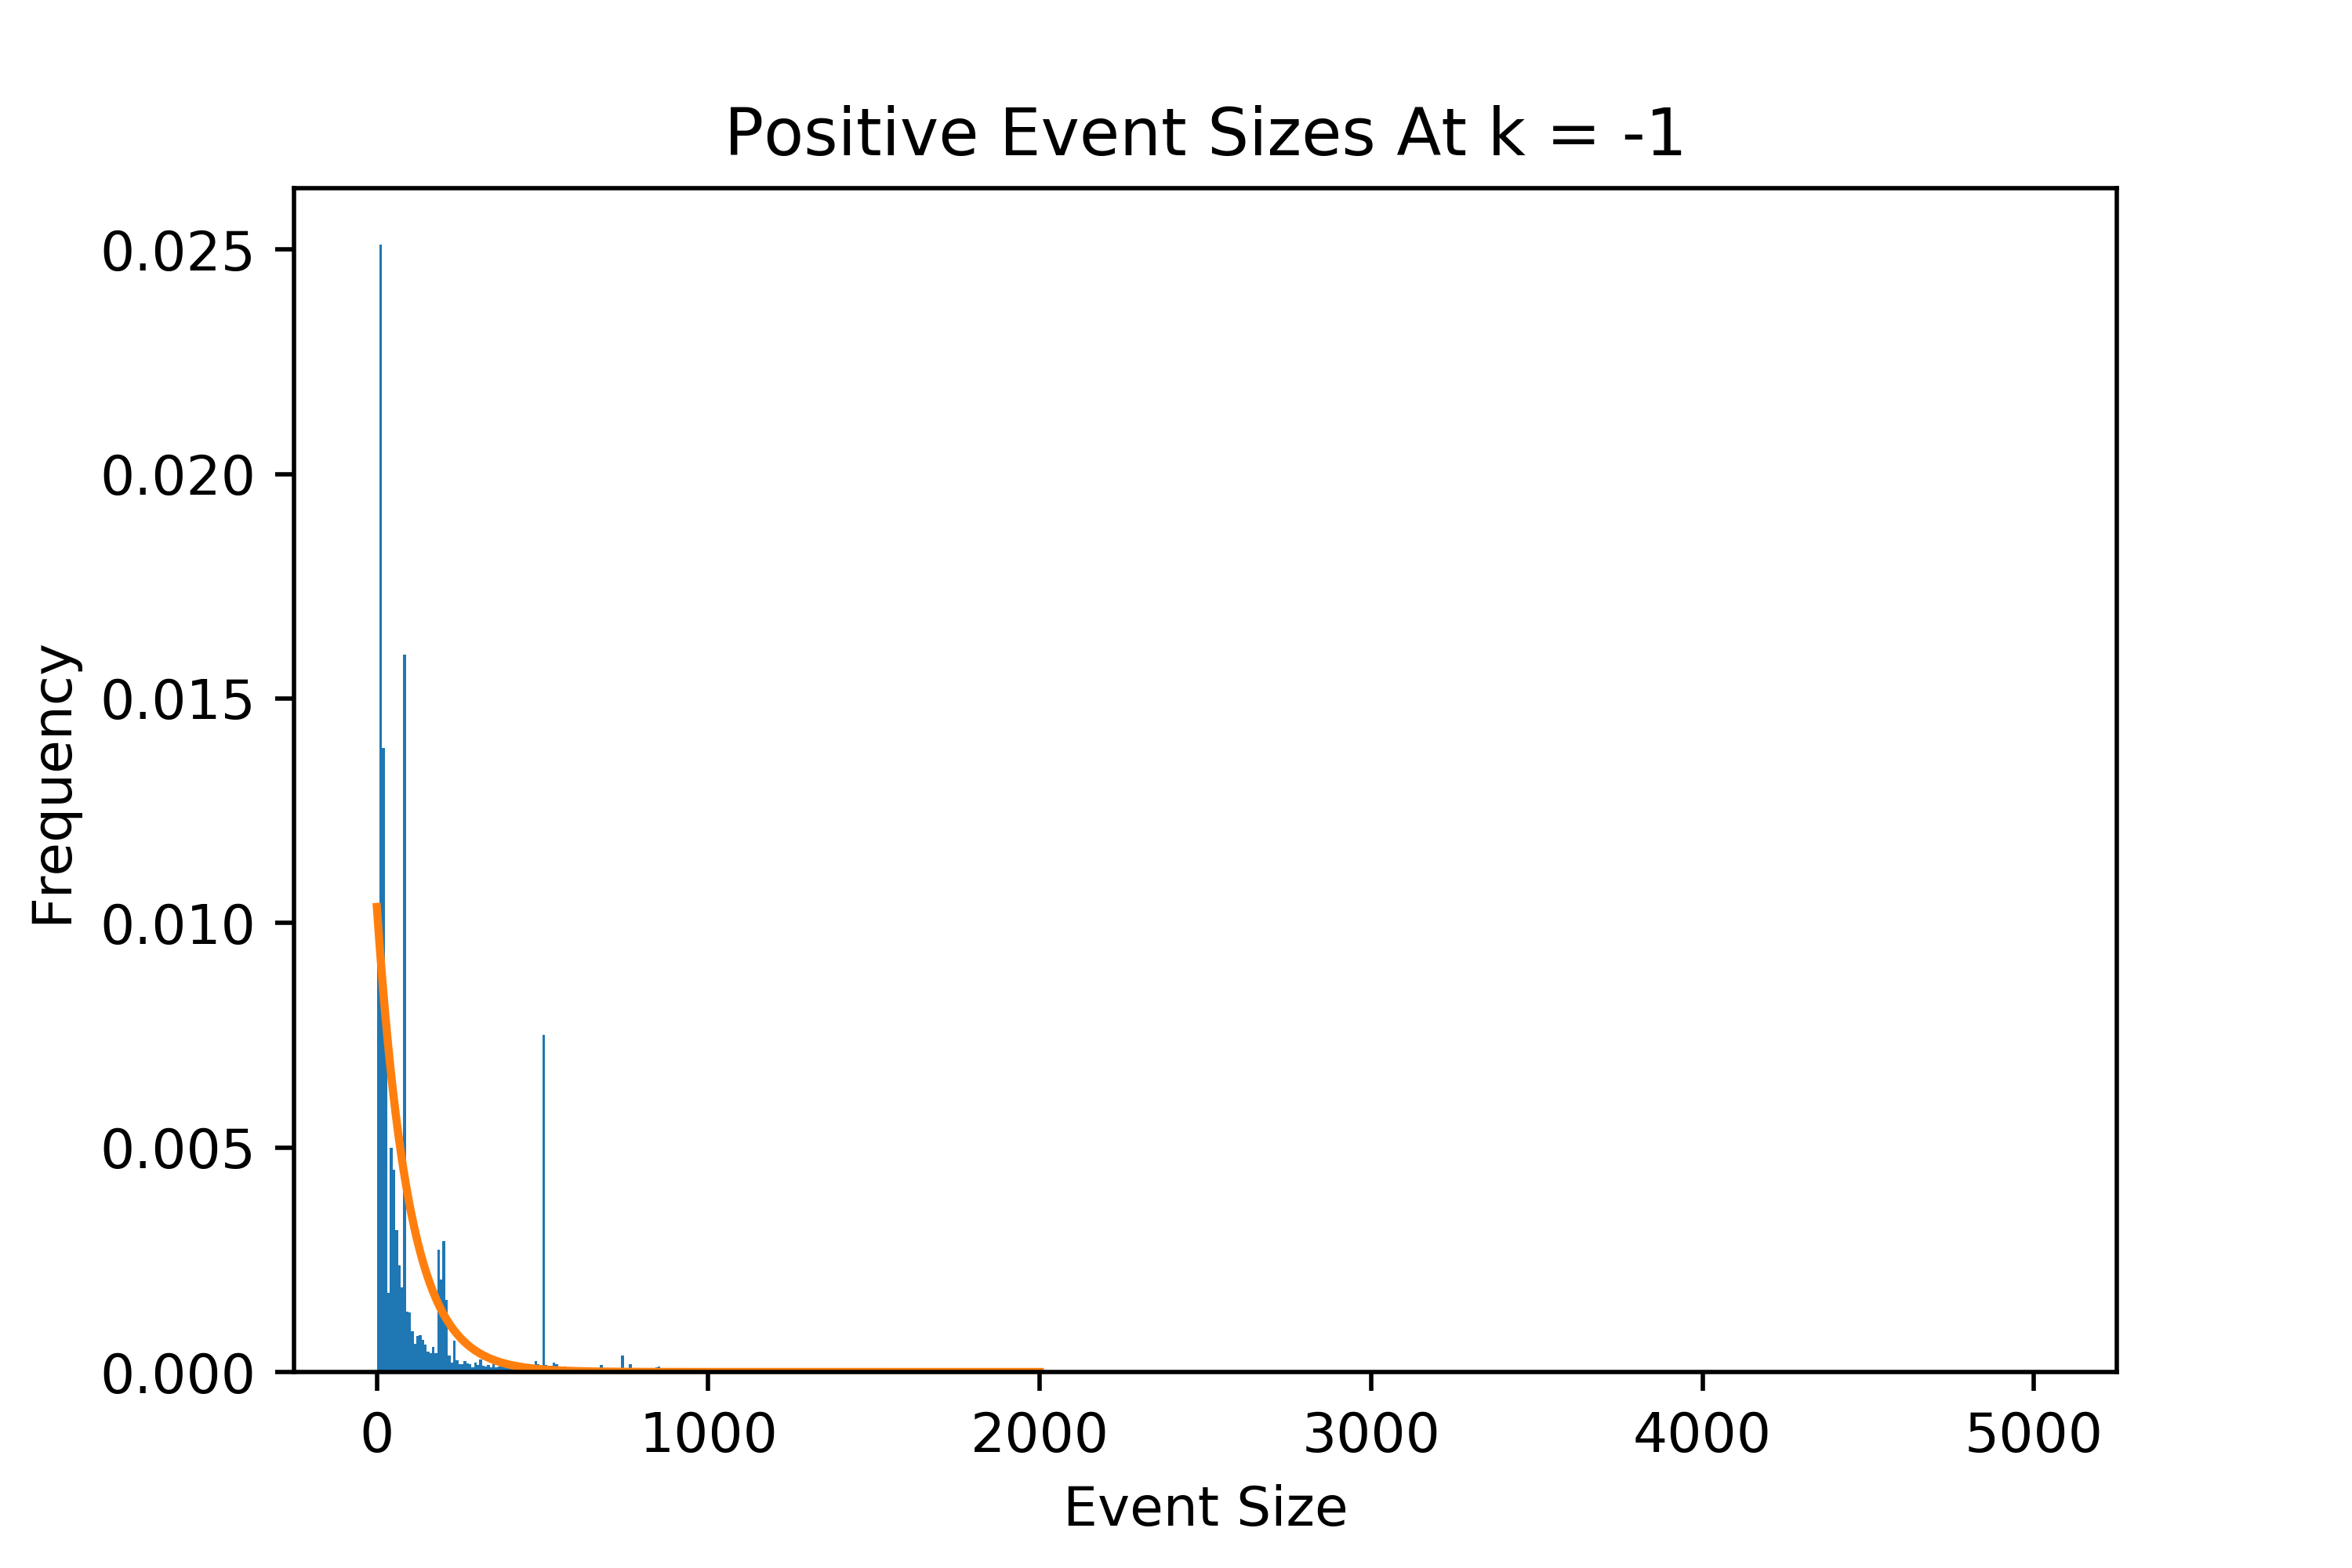
\includegraphics[width=60mm]{Figures/pos_-1.png}}
{}
&
\subf{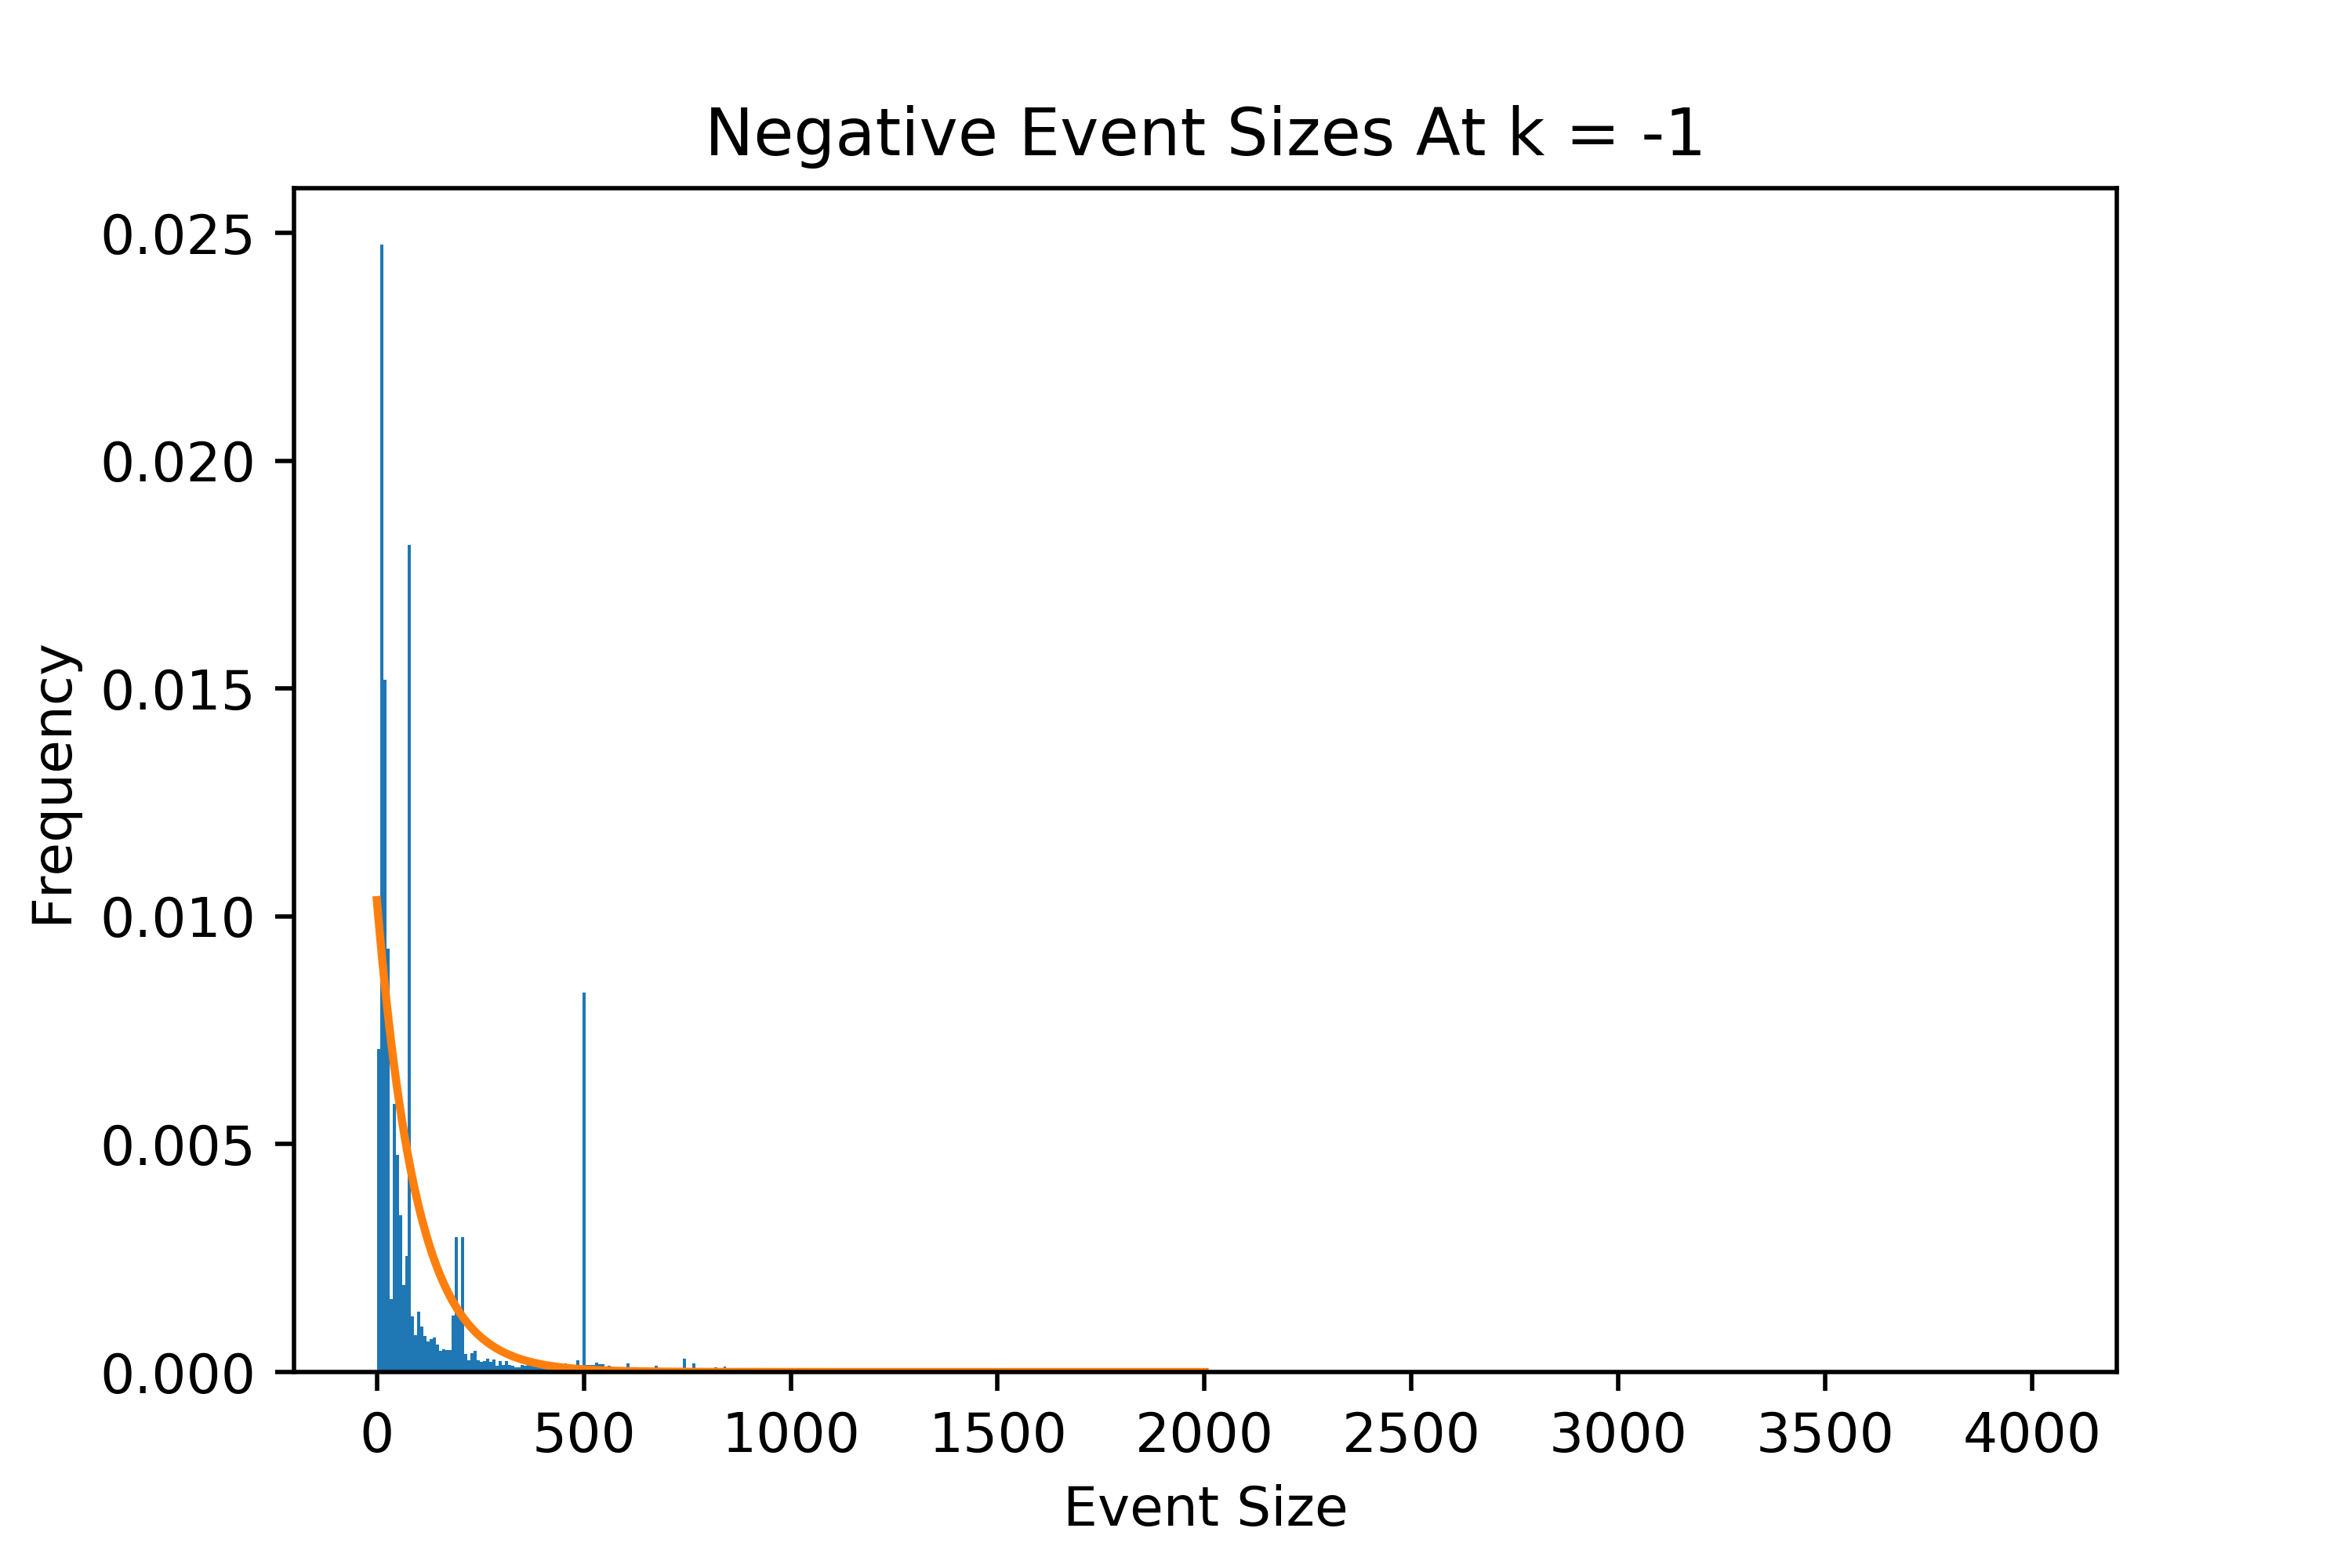
\includegraphics[width=60mm]{Figures/neg_-1.png}}
{}
\\
\subf{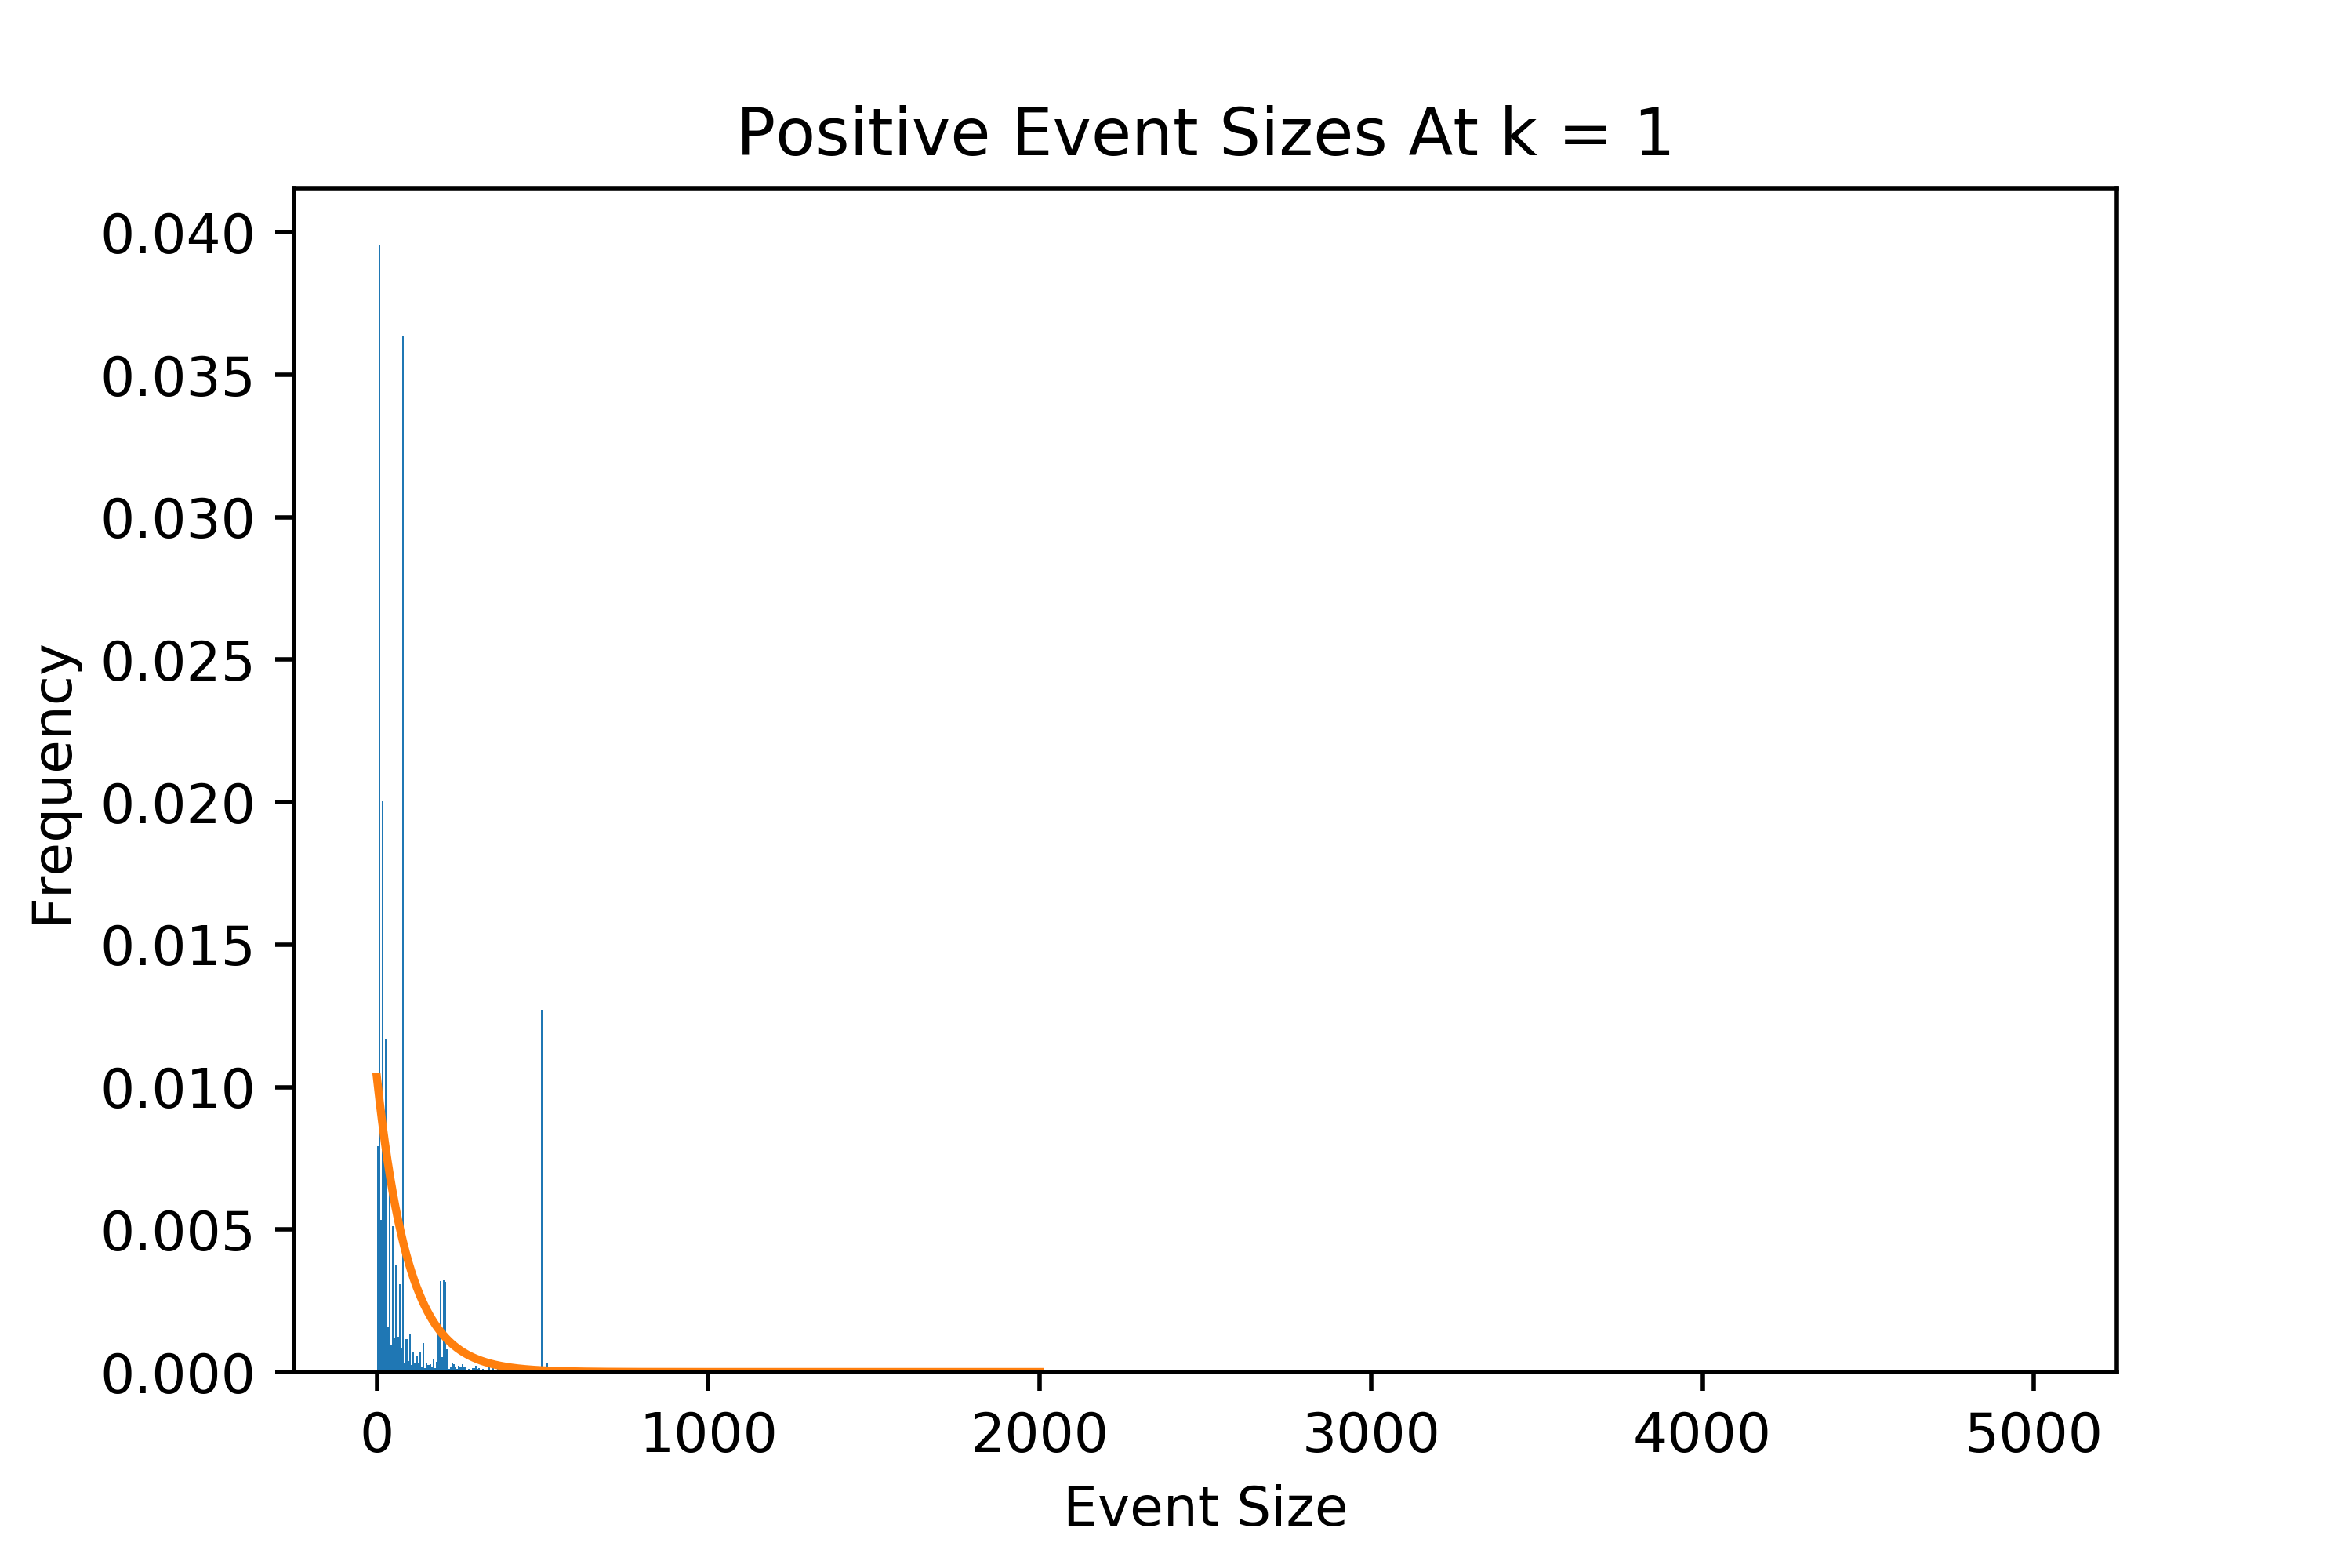
\includegraphics[width=60mm]{Figures/pos_1.png}}
{}
&
\subf{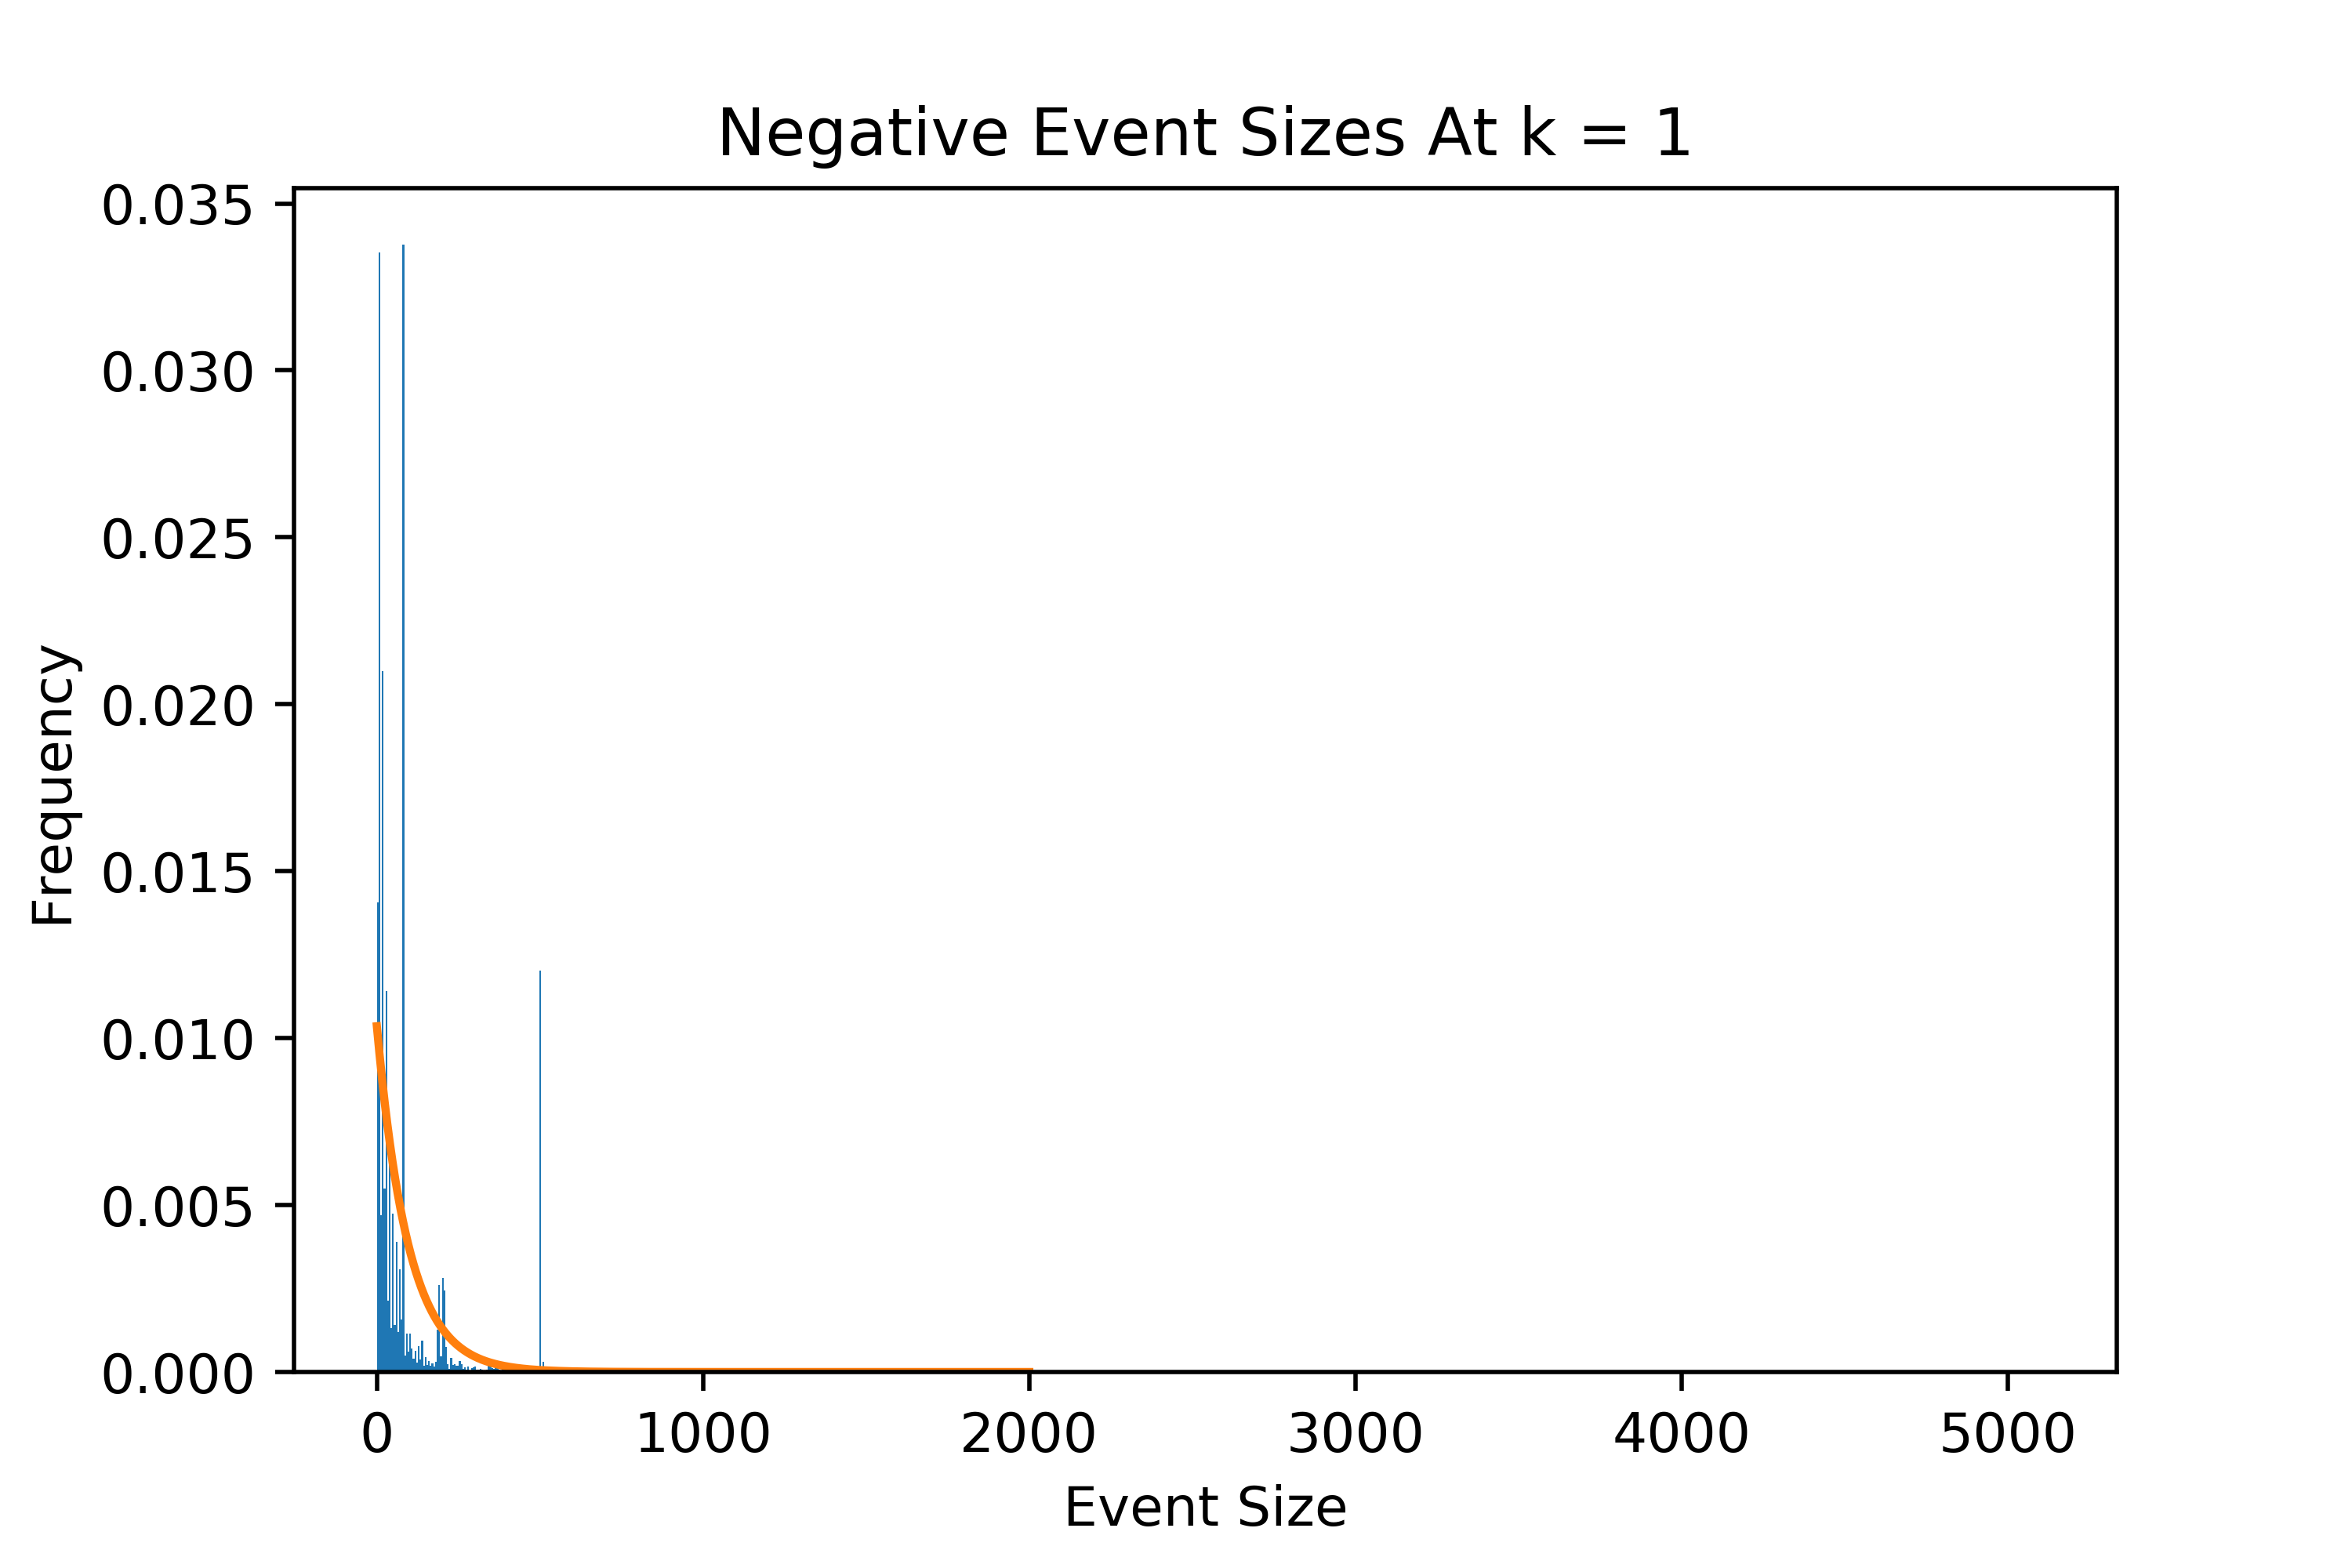
\includegraphics[width=60mm]{Figures/neg_1.png}}
{}
\\
\subf{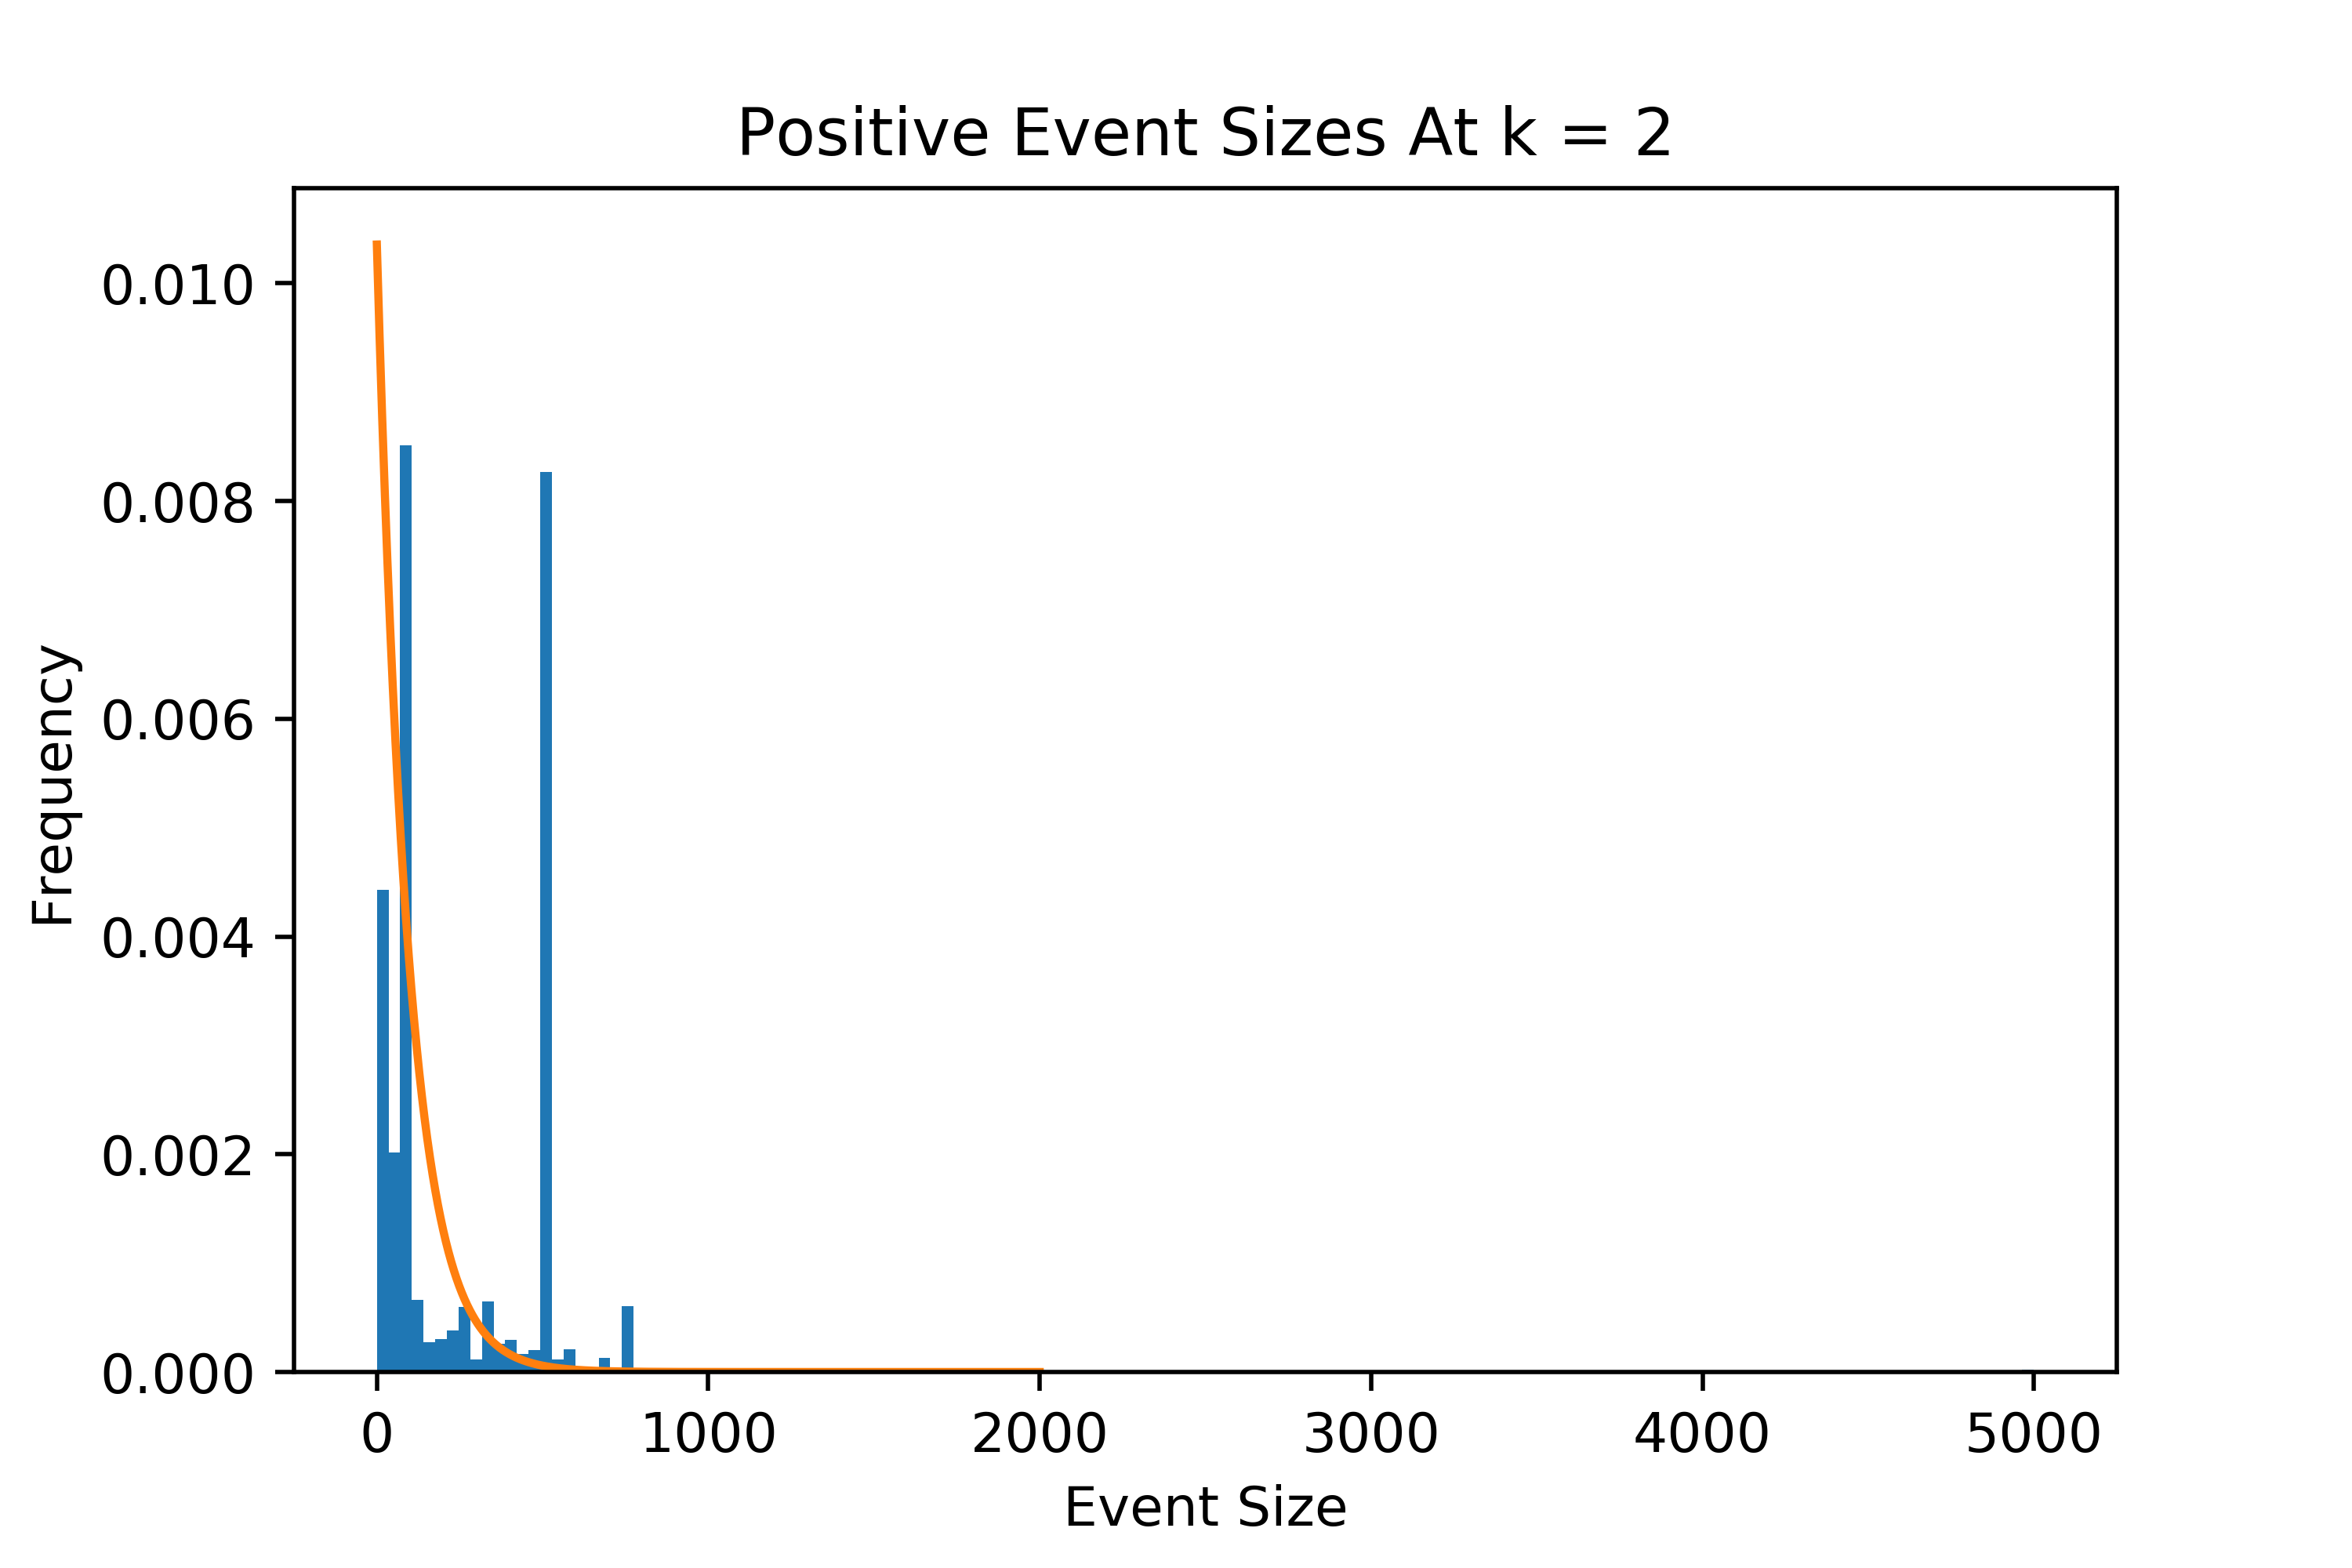
\includegraphics[width=60mm]{Figures/pos_2.png}}
{}
&
\subf{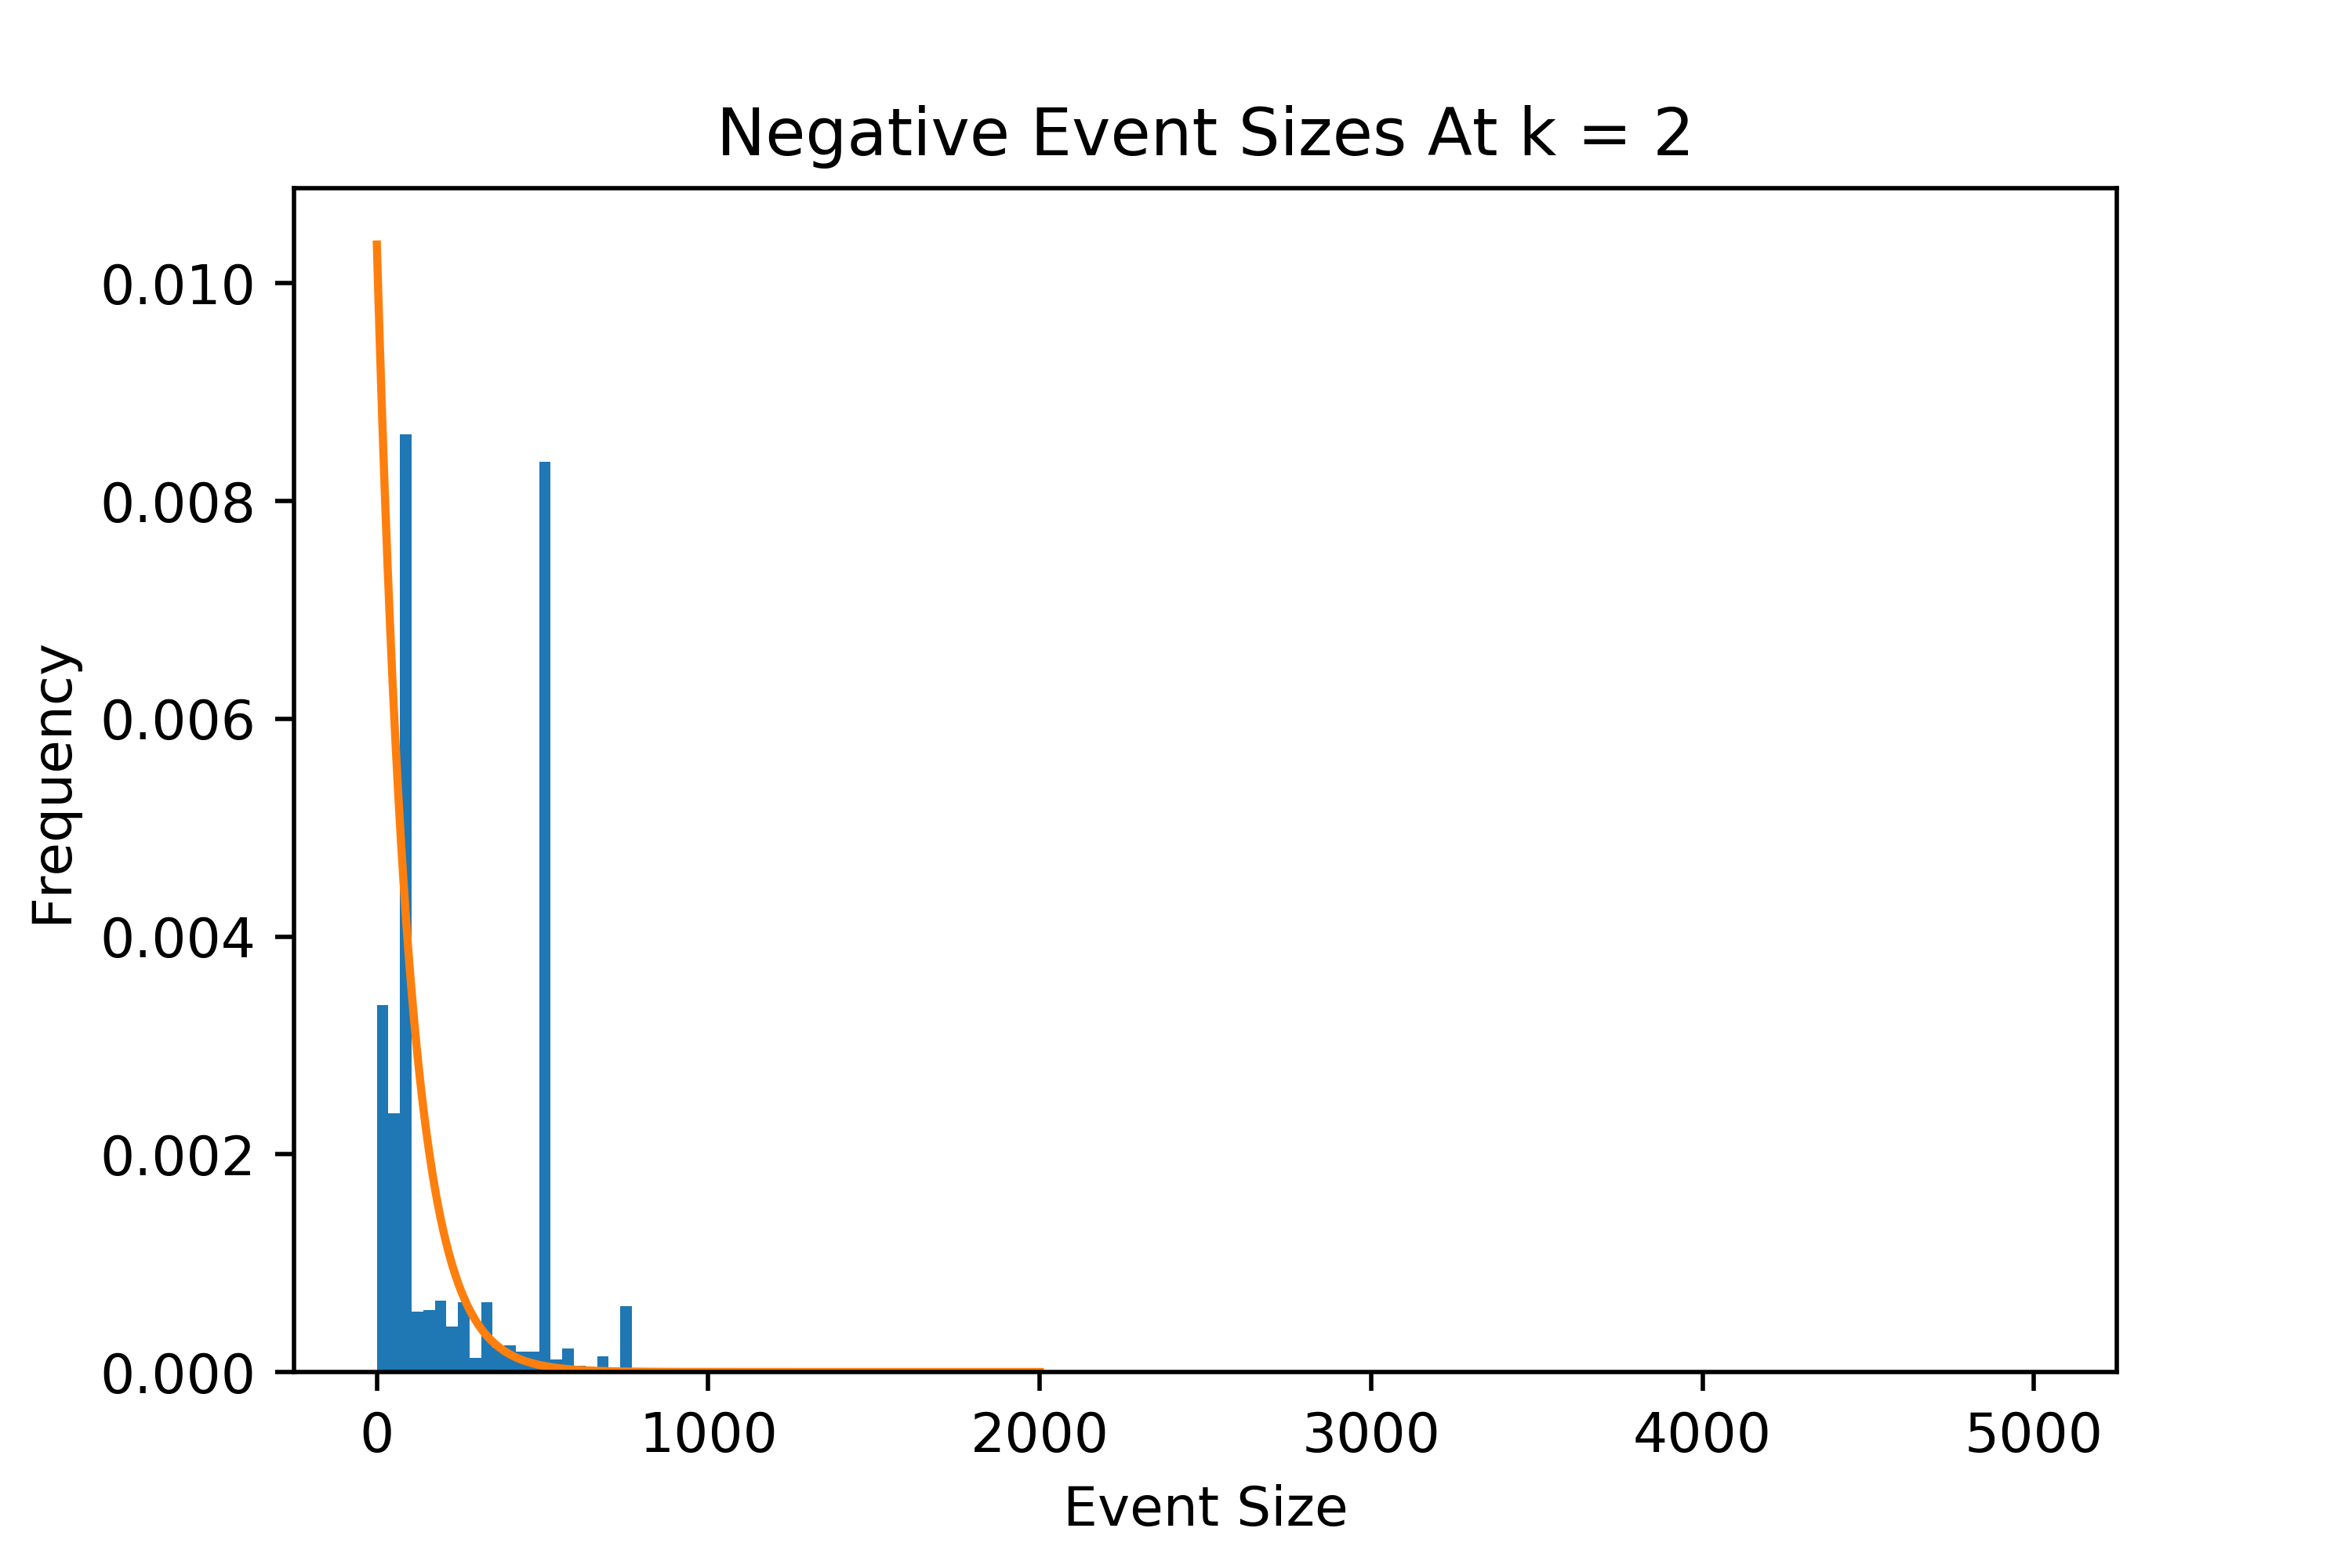
\includegraphics[width=60mm]{Figures/neg_2.png}}
{}
\\
\hline
\end{tabular}
\label{fig:sizes}
\end{figure}

As can be seen from Figure \ref{fig:sizes}, the exponential distribution with the mean rate as the $AES$ fits the data relatively well. However, there are some discrepancies such as the large frequency of orders at 500. A possible explanation for this is a trader splitting up a trade into equally sized amounts. There are also a non-negligible of orders near 5000 since that is the upper limit order size imposed by Coinbase. I choose to ignore these discrepancies so that the model can be more broadly applicable, but it may be possible to more accurately model the dynamics of the ETC-USD Coinbase Pro LOB with these taken into account. The $AES$ is reported for $K=10$ in table \ref{tab:AES}. It can be seen that in general, as the price gets closer to the reference price, the $AES$ decreases, but the number of events increases.

\begin{table}[htbp]
\caption{Average Event Sizes using Data from December 30, 2018} \label{tab:AES}
\begin{center}
\begin{tabular}{l|ll|ll}
\hline \hline
 & \multicolumn{2}{l|}{\textbf{Positive Events}} & \multicolumn{2}{l}{\textbf{Negative Events}} \\
\hline
k & n           & $AES$          & n           & $AES$          \\
\hline
-10         & 138        & 536.72        & 205         & 550.86             \\
-9         & 276        & 331.13         & 302         & 280.93             \\
-8         & 388        & 534.59         & 430         & 659.51             \\
-7         & 1249        & 566.10         & 1207         & 577.19             \\
-6         & 4145        & 520.49         & 4017         & 537.98             \\
-5         & 7615        & 471.58         & 7655         & 470.21             \\
-4         & 8958        & 463.97         & 9115         & 453.16             \\
-3         & 11584        & 405.31         & 11837         & 399.33             \\
-2         & 19494        & 247.61         & 18324         & 269.66             \\
-1         & 20666        & 117.95         & 18028         & 121.73             \\
1         & 19064        & 96.56         & 18402         & 94.21             \\
2         & 13420        & 248.50         & 13641         & 255.25             \\
3         & 13214        & 356.71         & 13643         & 350.755             \\
4         & 15322        & 327.24         & 15119         & 335.16             \\
5         & 12444        & 325.70         & 12090         & 324.47             \\
6         & 4733        & 460.40         & 4588         & 466.64             \\
7         & 1466        & 620.93         & 1400         & 663.58             \\
8         & 428        & 562.84         & 410         & 545.73             \\
9         & 229        & 502.40         & 218        & 577.02             \\
10         & 168        & 340.23         & 174         & 287.10             \\
\end{tabular}
\end{center}
\end{table}

\subsection{Average Arrival Rates}\label{ch:poisson}
We first examine whether event arrivals at each position can be modelled as a Poisson process. To do so, I test whether the inter-arrival times of the events are exponentially distributed. It can be seen from the QQ-plots in Figures \ref{fig:interarrivals_pos} and \ref{fig:interarrivals_neg}, which compare the empirical distribution to an exponential distribution, that the inter-arrival times have heavy right tails compared to the exponential distribution. When I plot the histogram of inter-arrival times vs. the an exponential distribution, it can be seen that the exponential distribution fits the data well for the majority of the points except for a small number of outliers to the right. Despite this discrepancy, I choose to model the arrival as a Poisson process because the number of outliers is small and for its desirable properties for ease of simulation. I report the average rates $\lambda^+_k$ and $\lambda^-_k$ for $K=10$ in Table \ref{tab:rates}

\begin{table}[htbp]
\caption{Average Arrival Rates ($s^{-1}$) using Data from December 30, 2018} \label{tab:rates}
\begin{center}
\begin{tabular}{l|l|l}
\hline 
k & $\lambda^+_k$           & $\lambda^-_k$         \\
\hline
-10         & 0.001597        & 0.002373  \\
-9         & 0.003194        & 0.0034952  \\
-8         & 0.004491        & 0.004977  \\
-7         & 0.01446        & 0.01397  \\
-6         & 0.04797        & 0.04649  \\
-5         & 0.08813        & 0.08860  \\
-4         & 0.1037        & 0.1055  \\
-3         & 0.1341        & 0.1370  \\
-2         & 0.2256        & 0.2121  \\
-1         & 0.2392        & 0.2087  \\
1         & 0.2206        & 0.2130  \\
2         & 0.1553        & 0.1579  \\
3           & 0.1529        & 0.1579  \\
4         & 0.1773        & 0.1750  \\
5         & 0.1440        & 0.1399  \\
6         & 0.05478        & 0.05310  \\
7         & 0.01697        & 0.01620  \\
8         & 0.004954        & 0.004745 \\
9         &  0.002650        & 0.002523  \\
10         & 0.001944        & 0.002014  \\
\end{tabular}
\end{center}
\end{table}


\begin{figure}
\centering
\caption{Inter-Arrival Times Compared to Exponential Distribution using Data from December 30, 2018}
\begin{tabular}{cc}
\hline
\subf{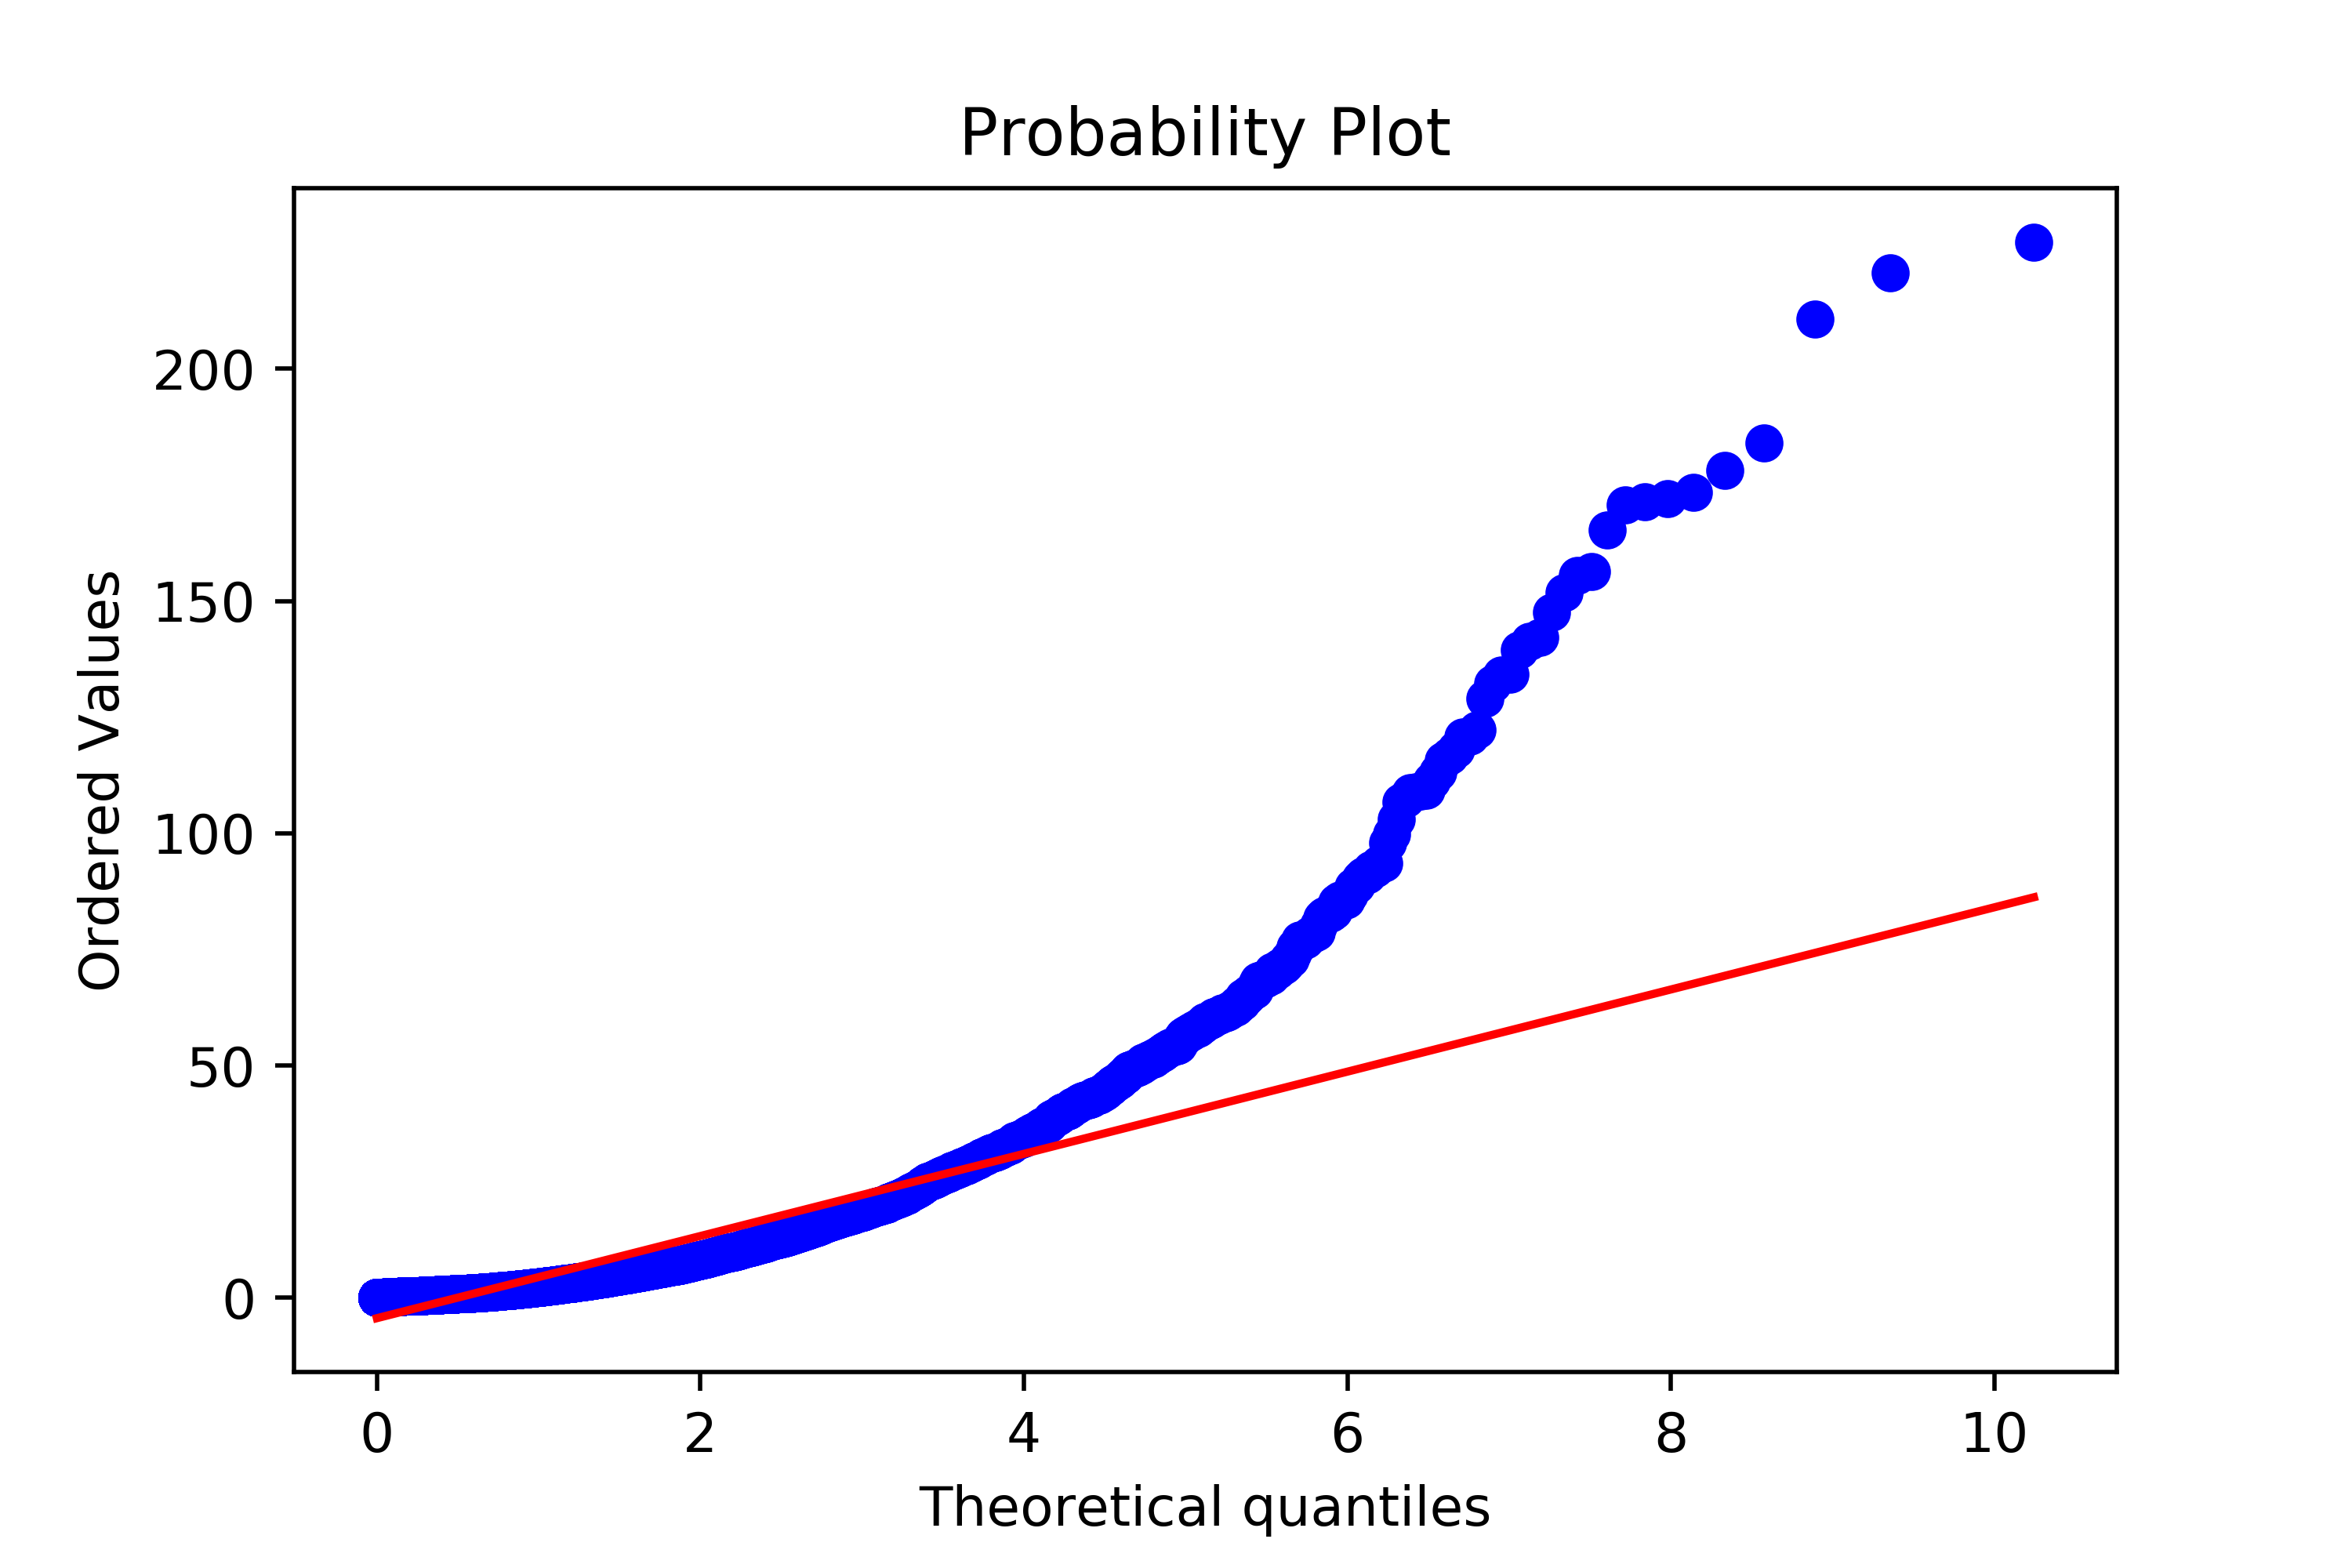
\includegraphics[width=60mm]{Figures/QQ_pos_k-2.png}}
{}
&
\subf{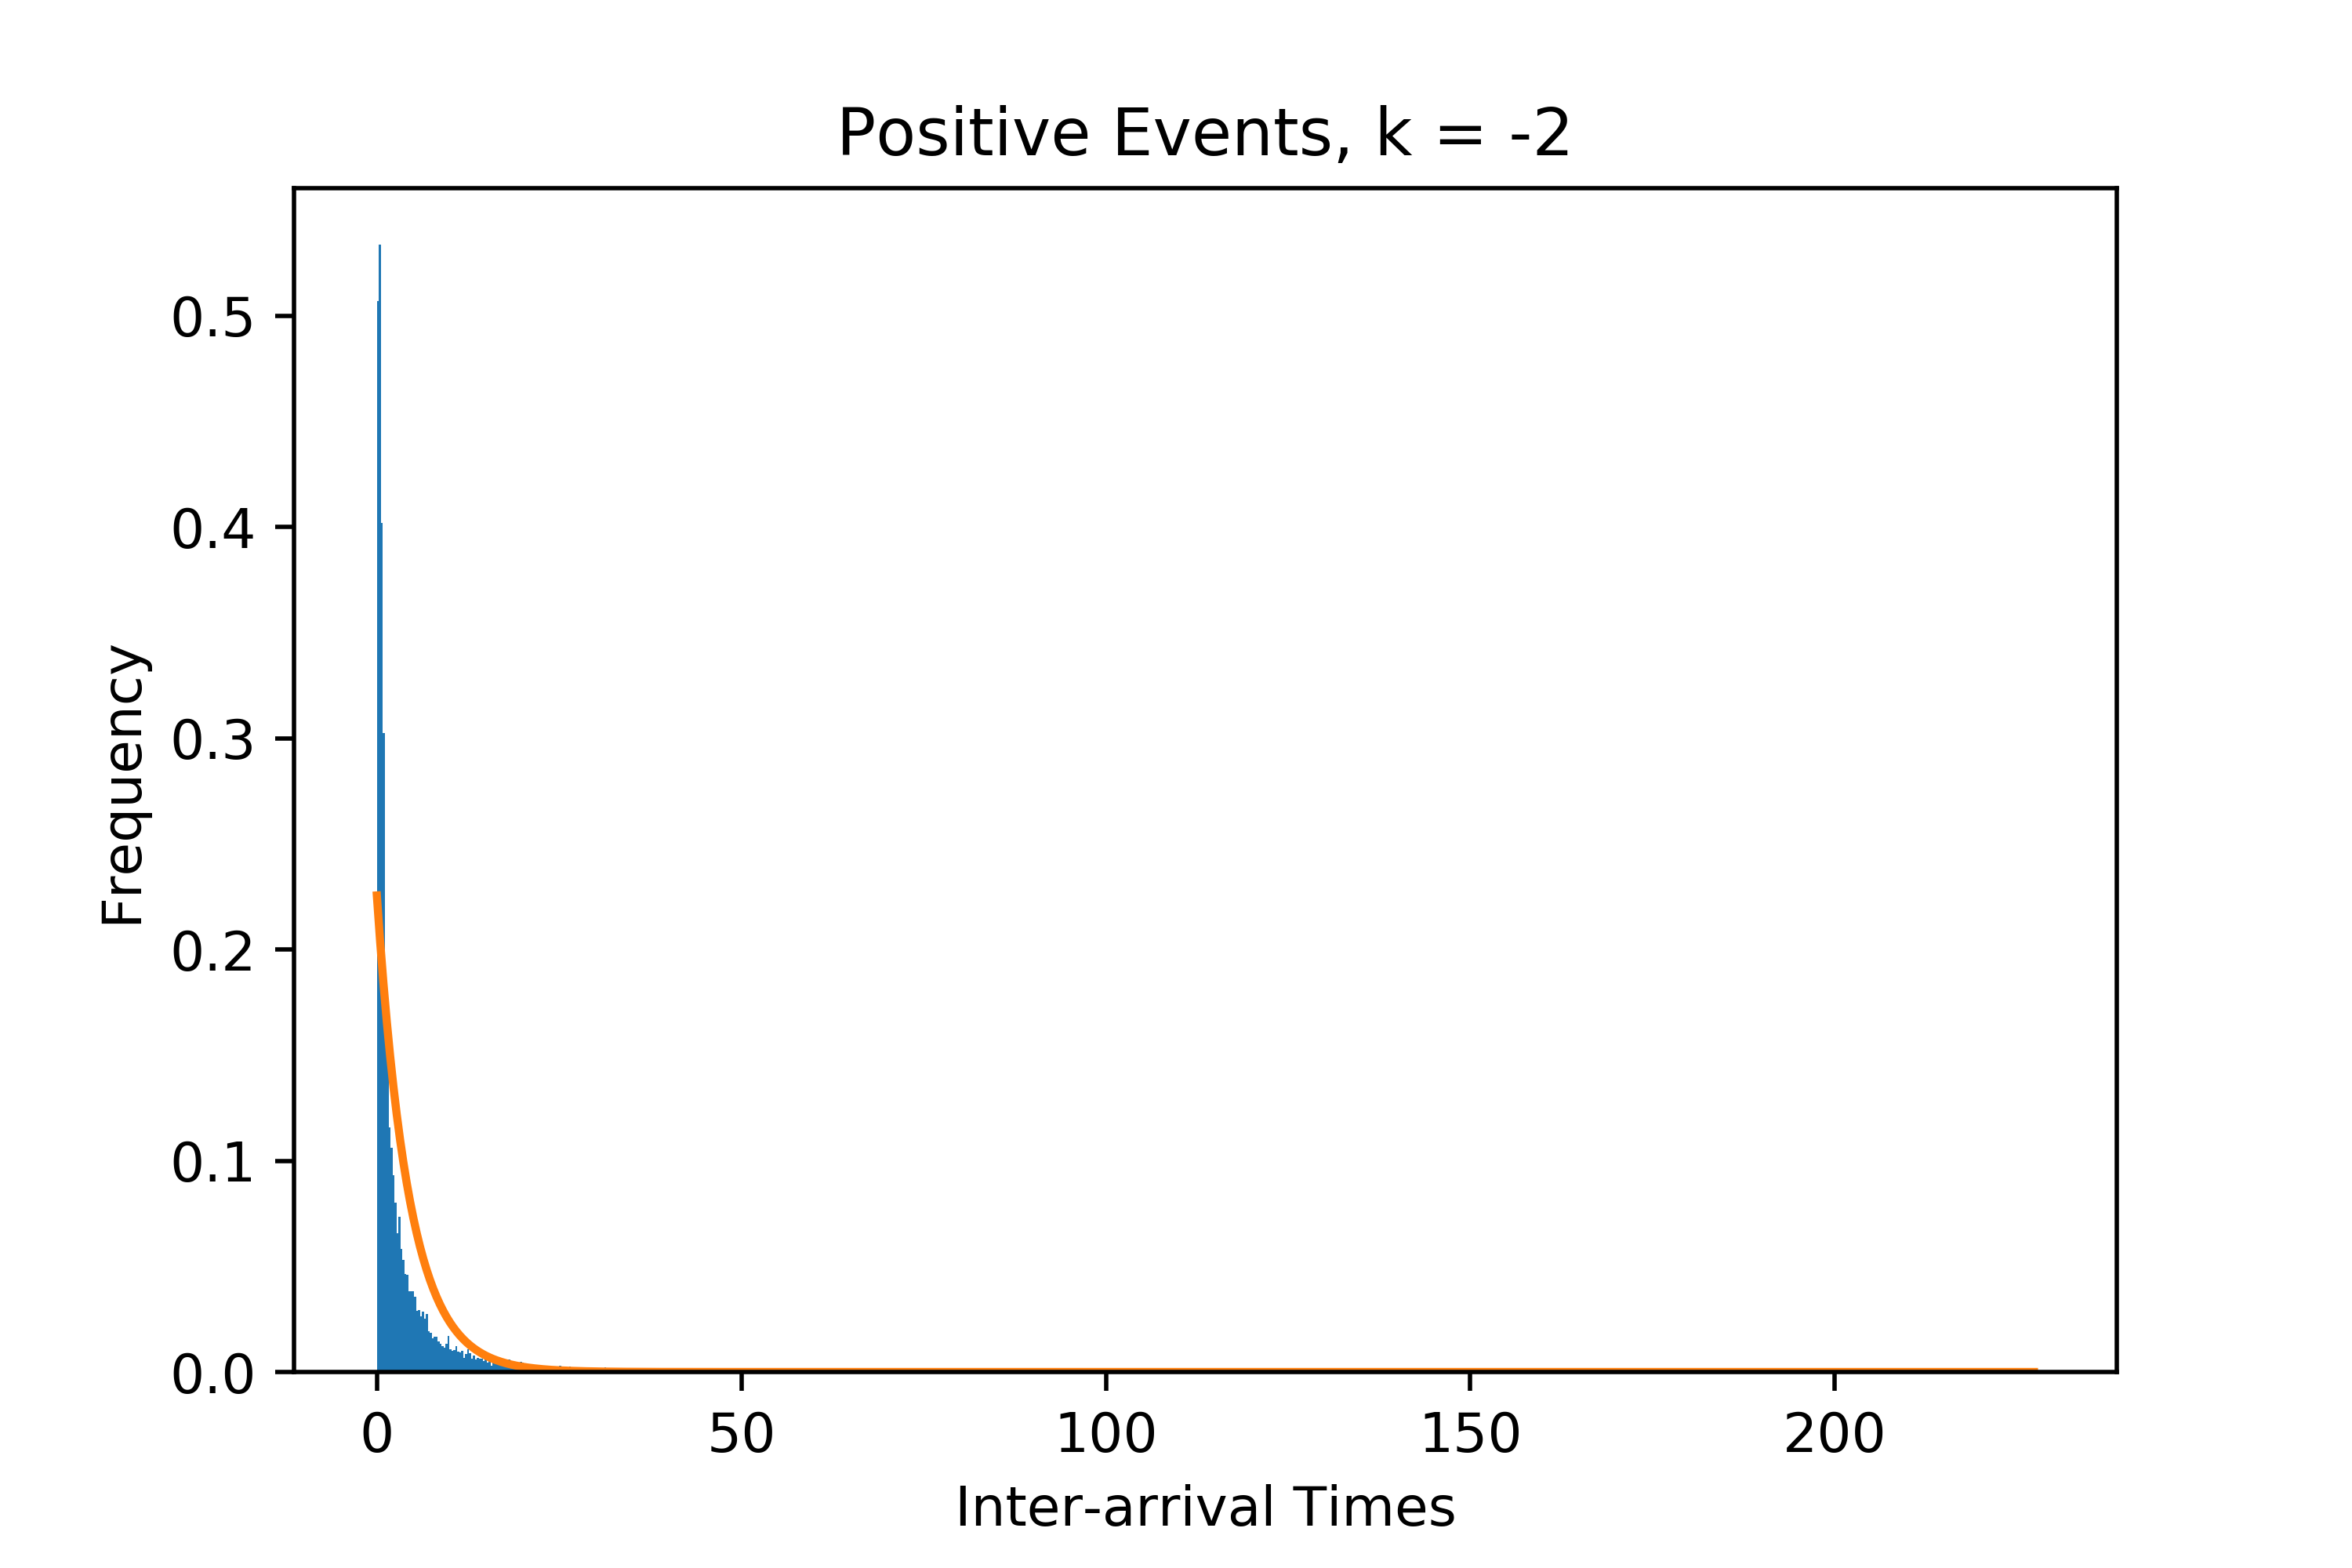
\includegraphics[width=60mm]{Figures/hist_pos_k-2.png}}
{}
\\
\subf{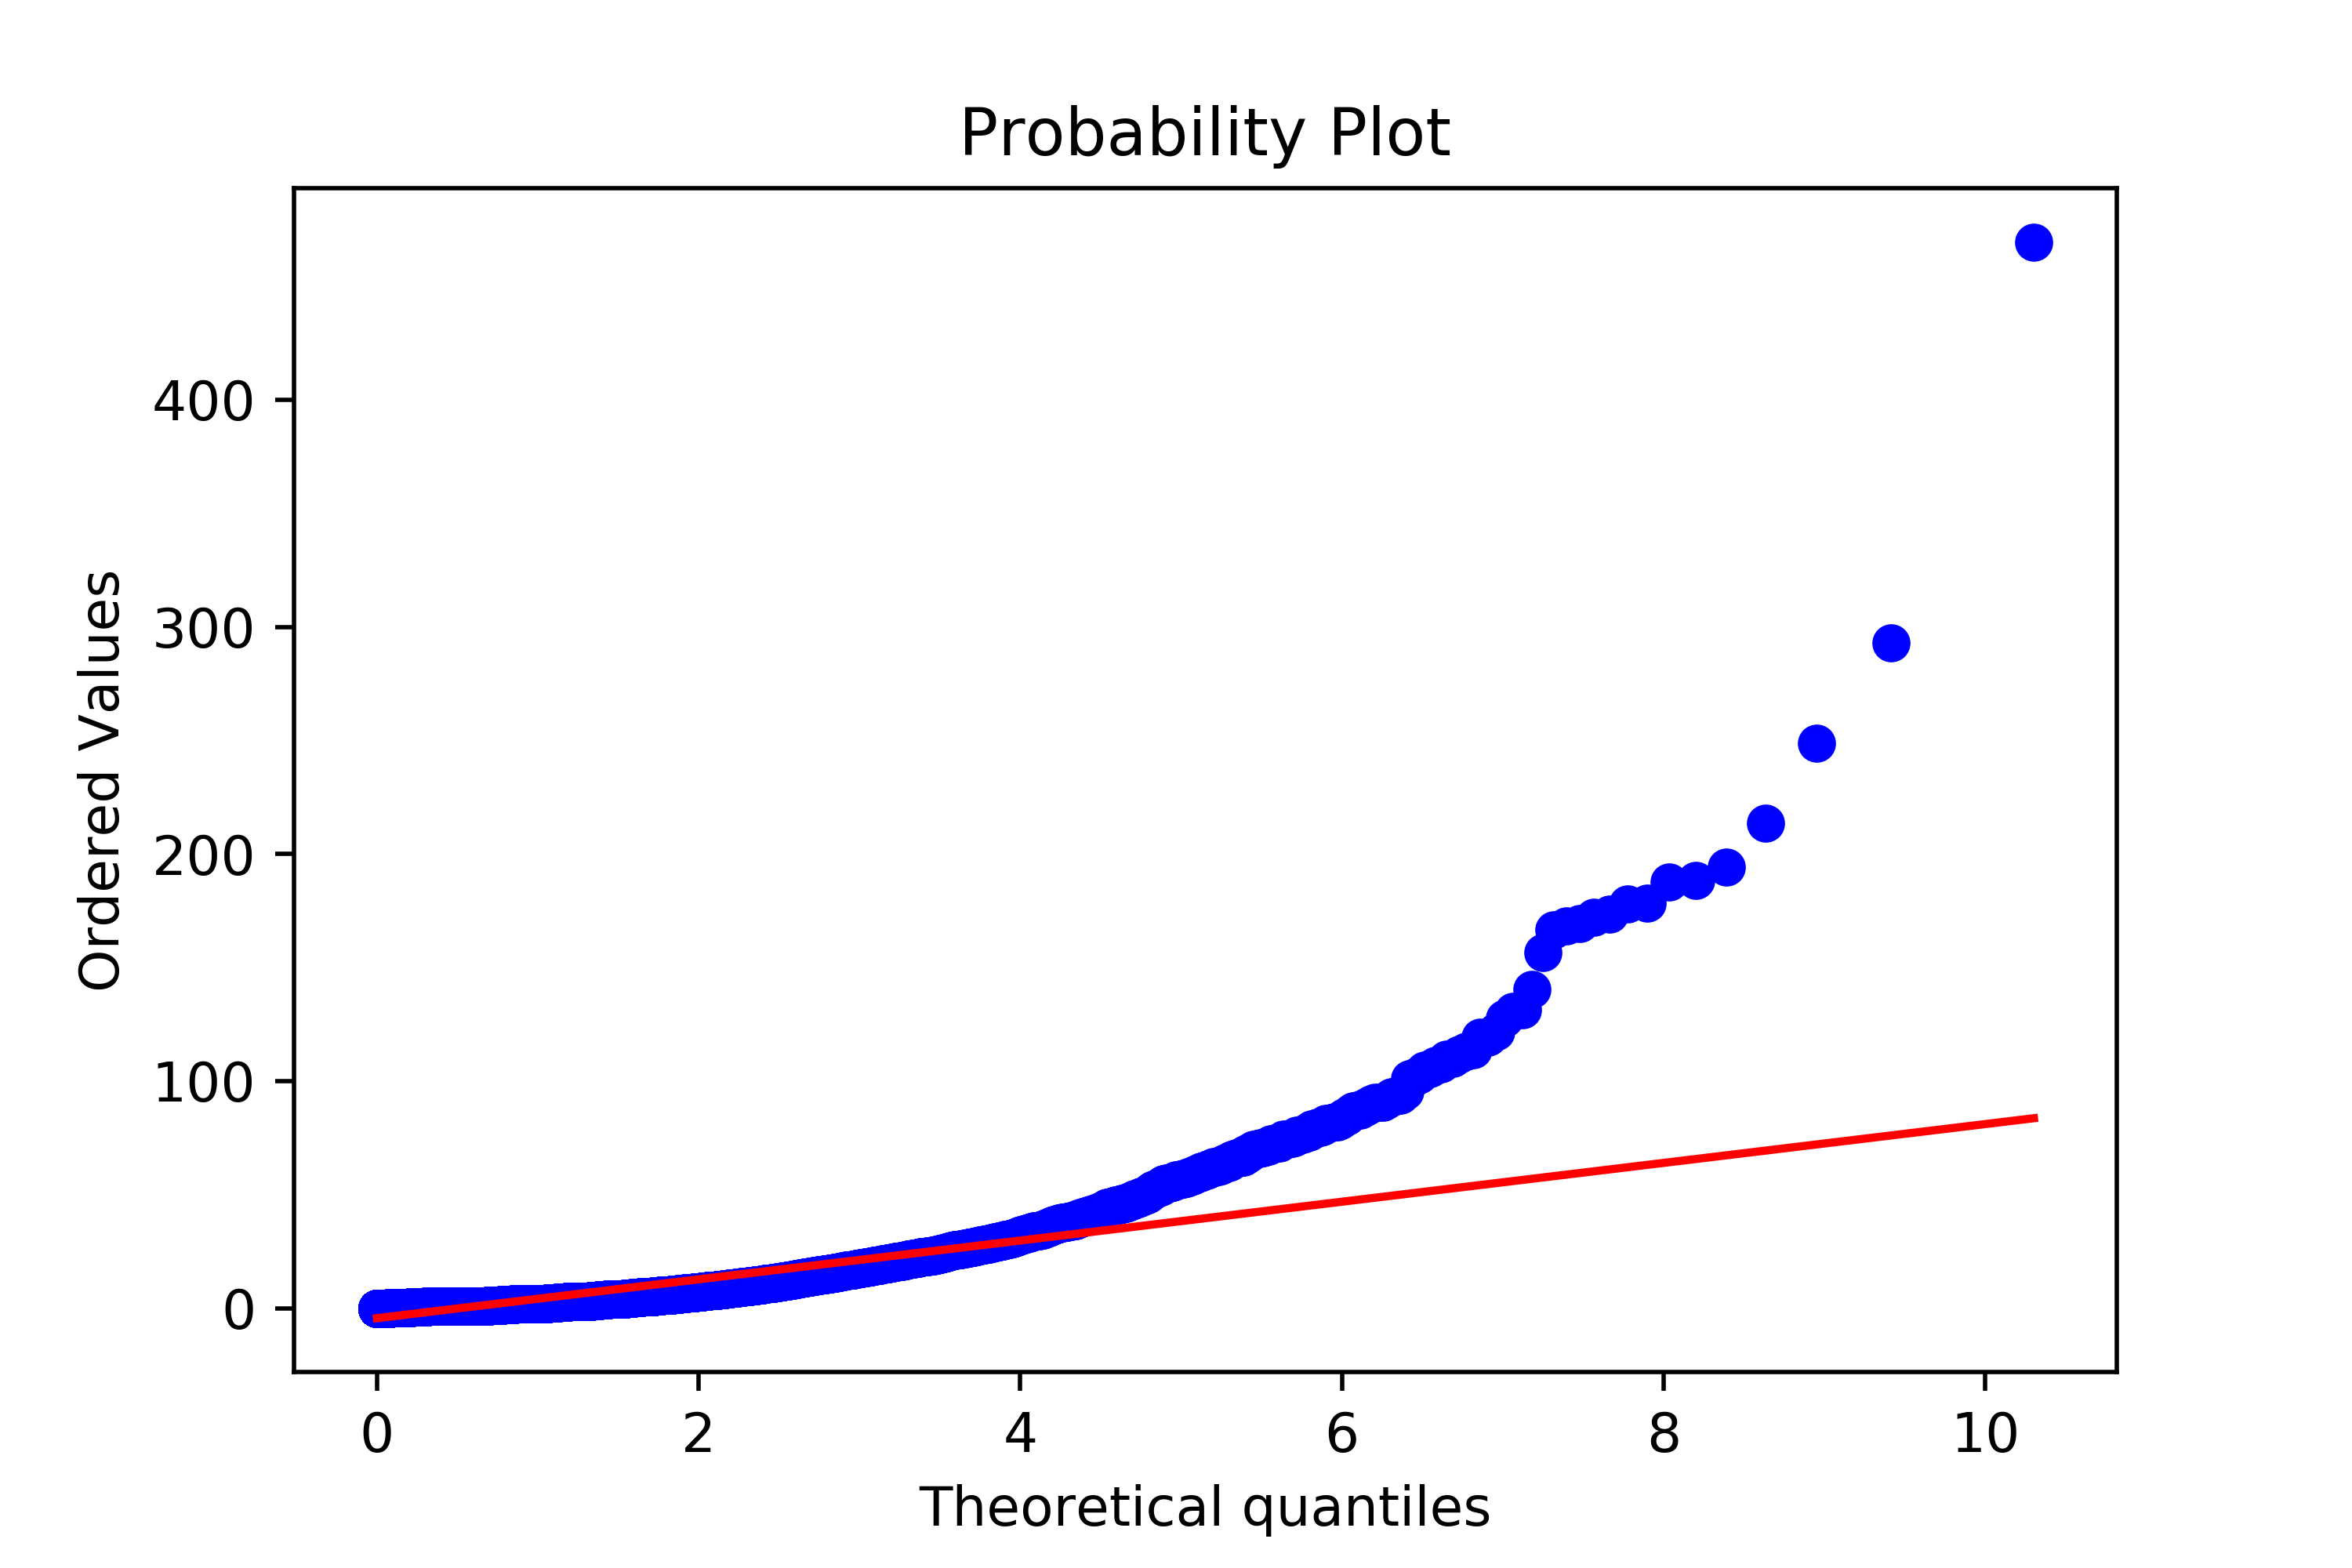
\includegraphics[width=60mm]{Figures/QQ_pos_k-1.png}}
{}
&
\subf{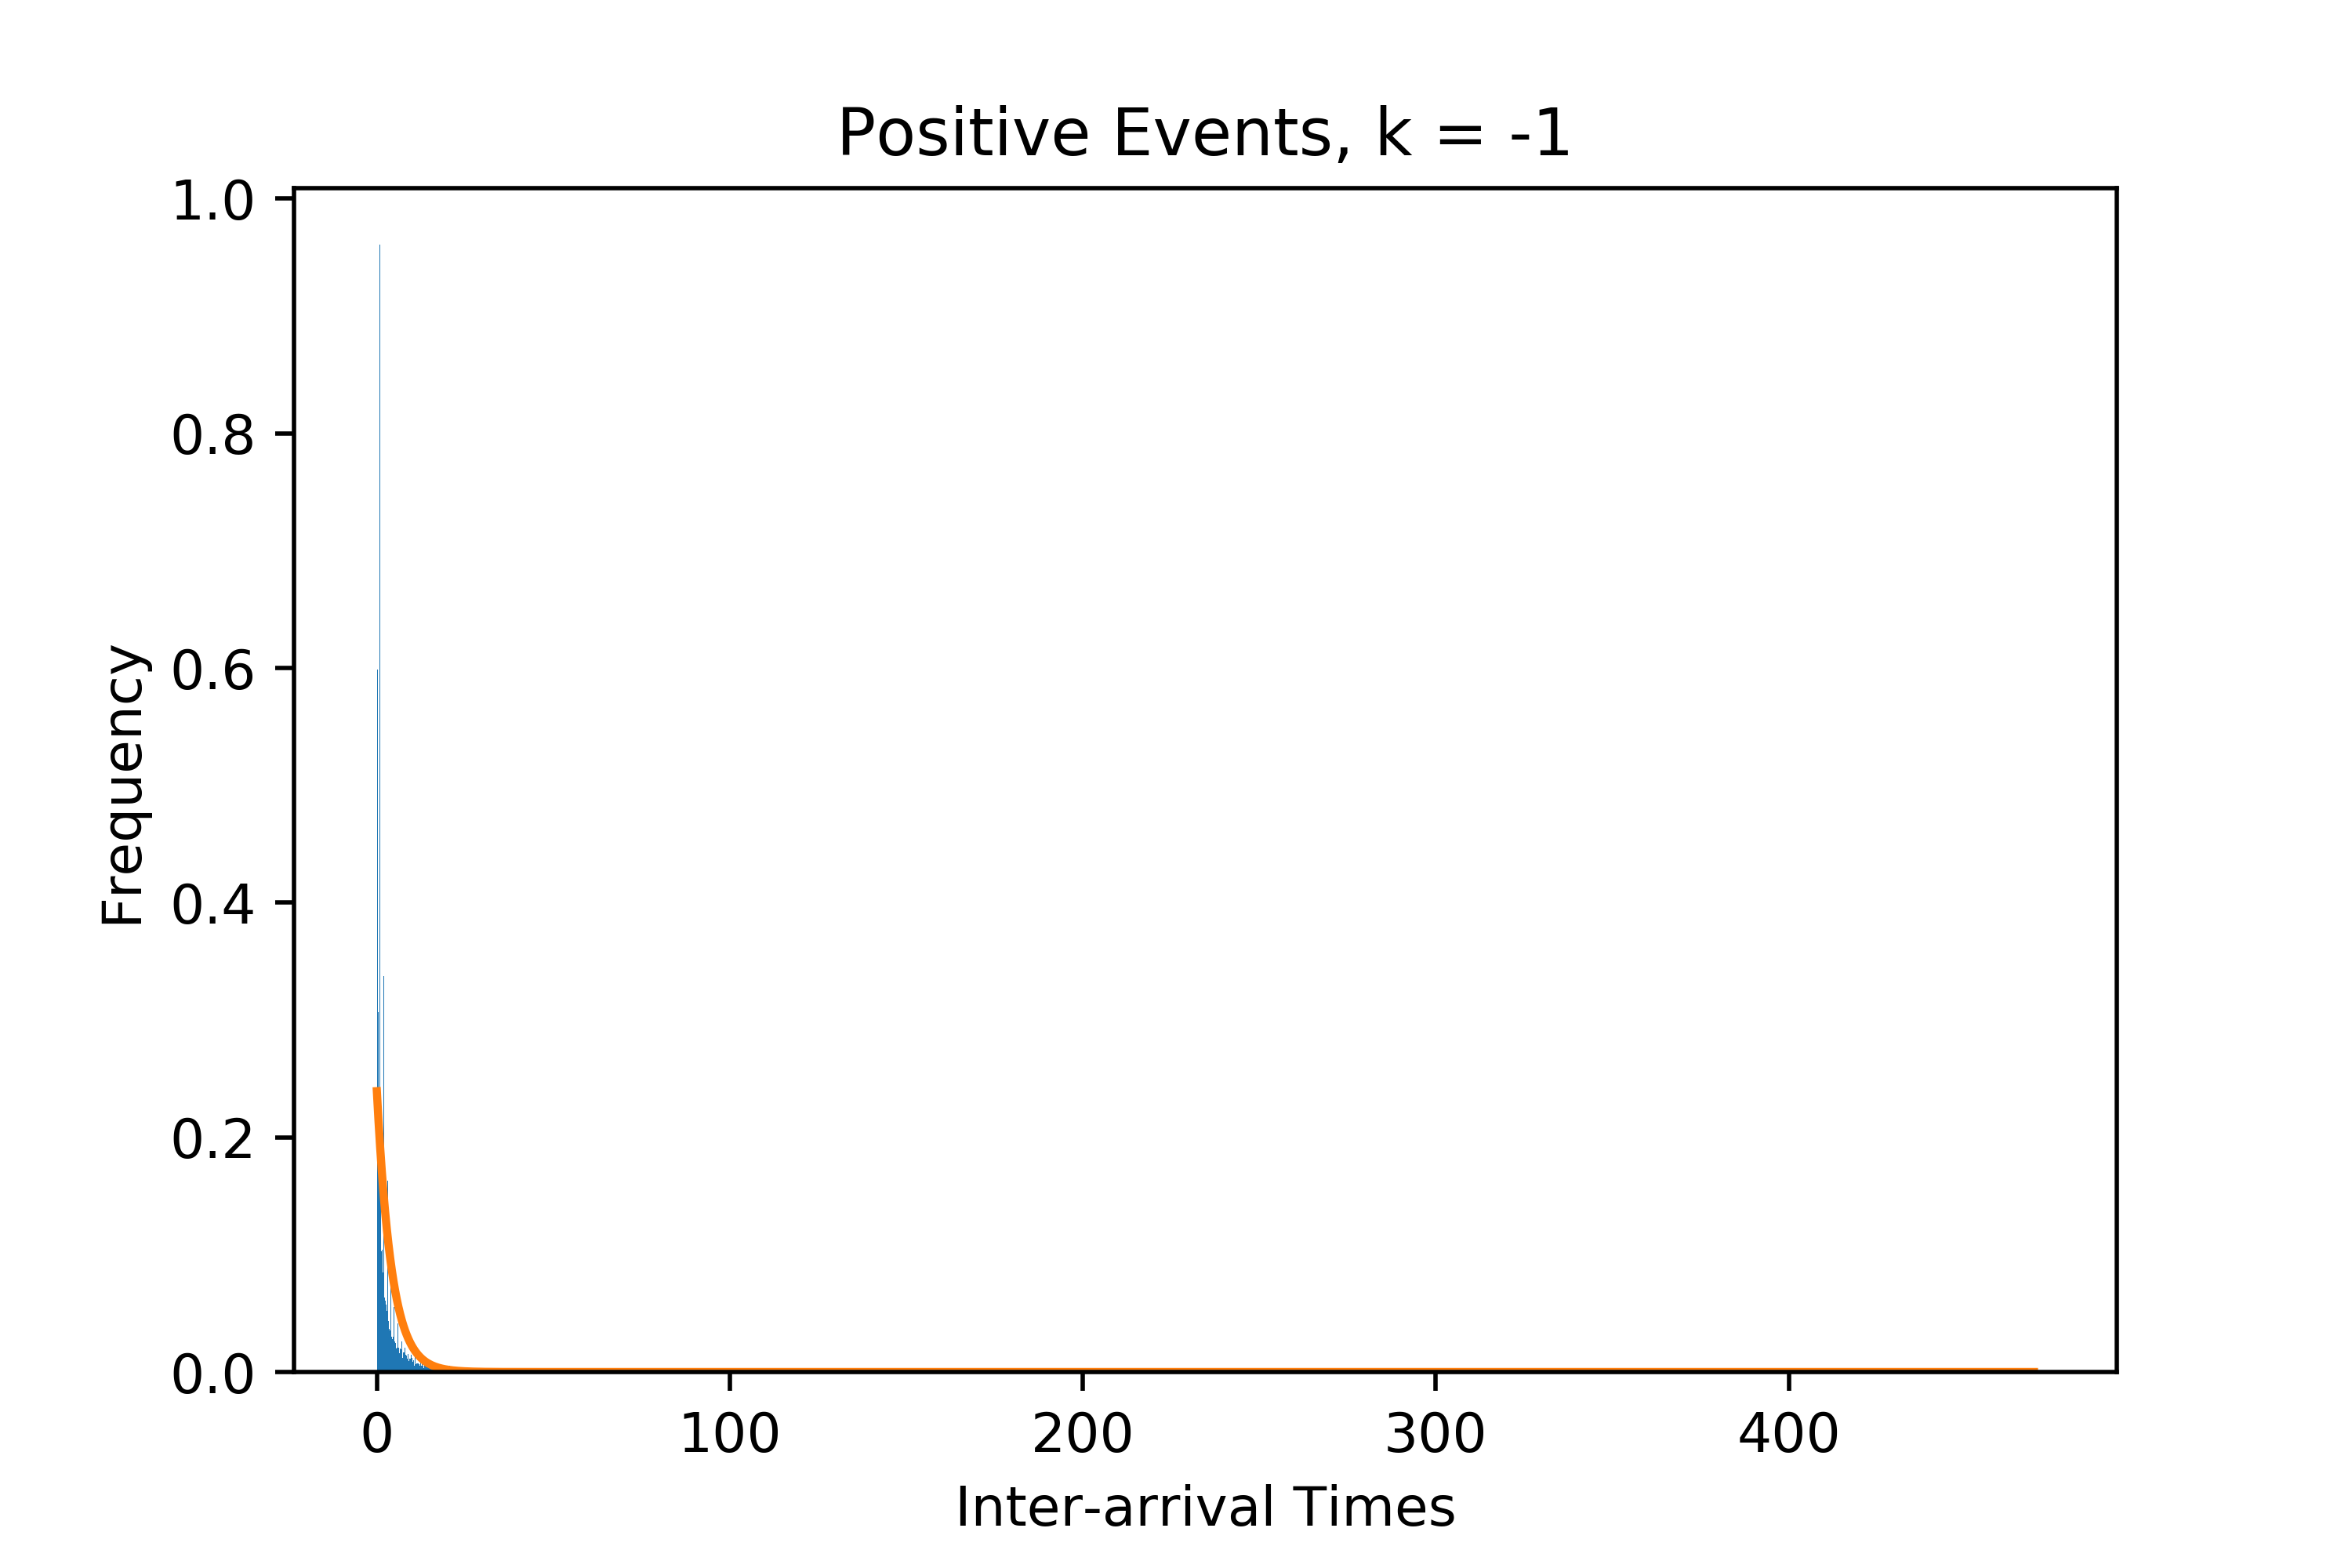
\includegraphics[width=60mm]{Figures/hist_pos_k-1.png}}
{}
\\
\subf{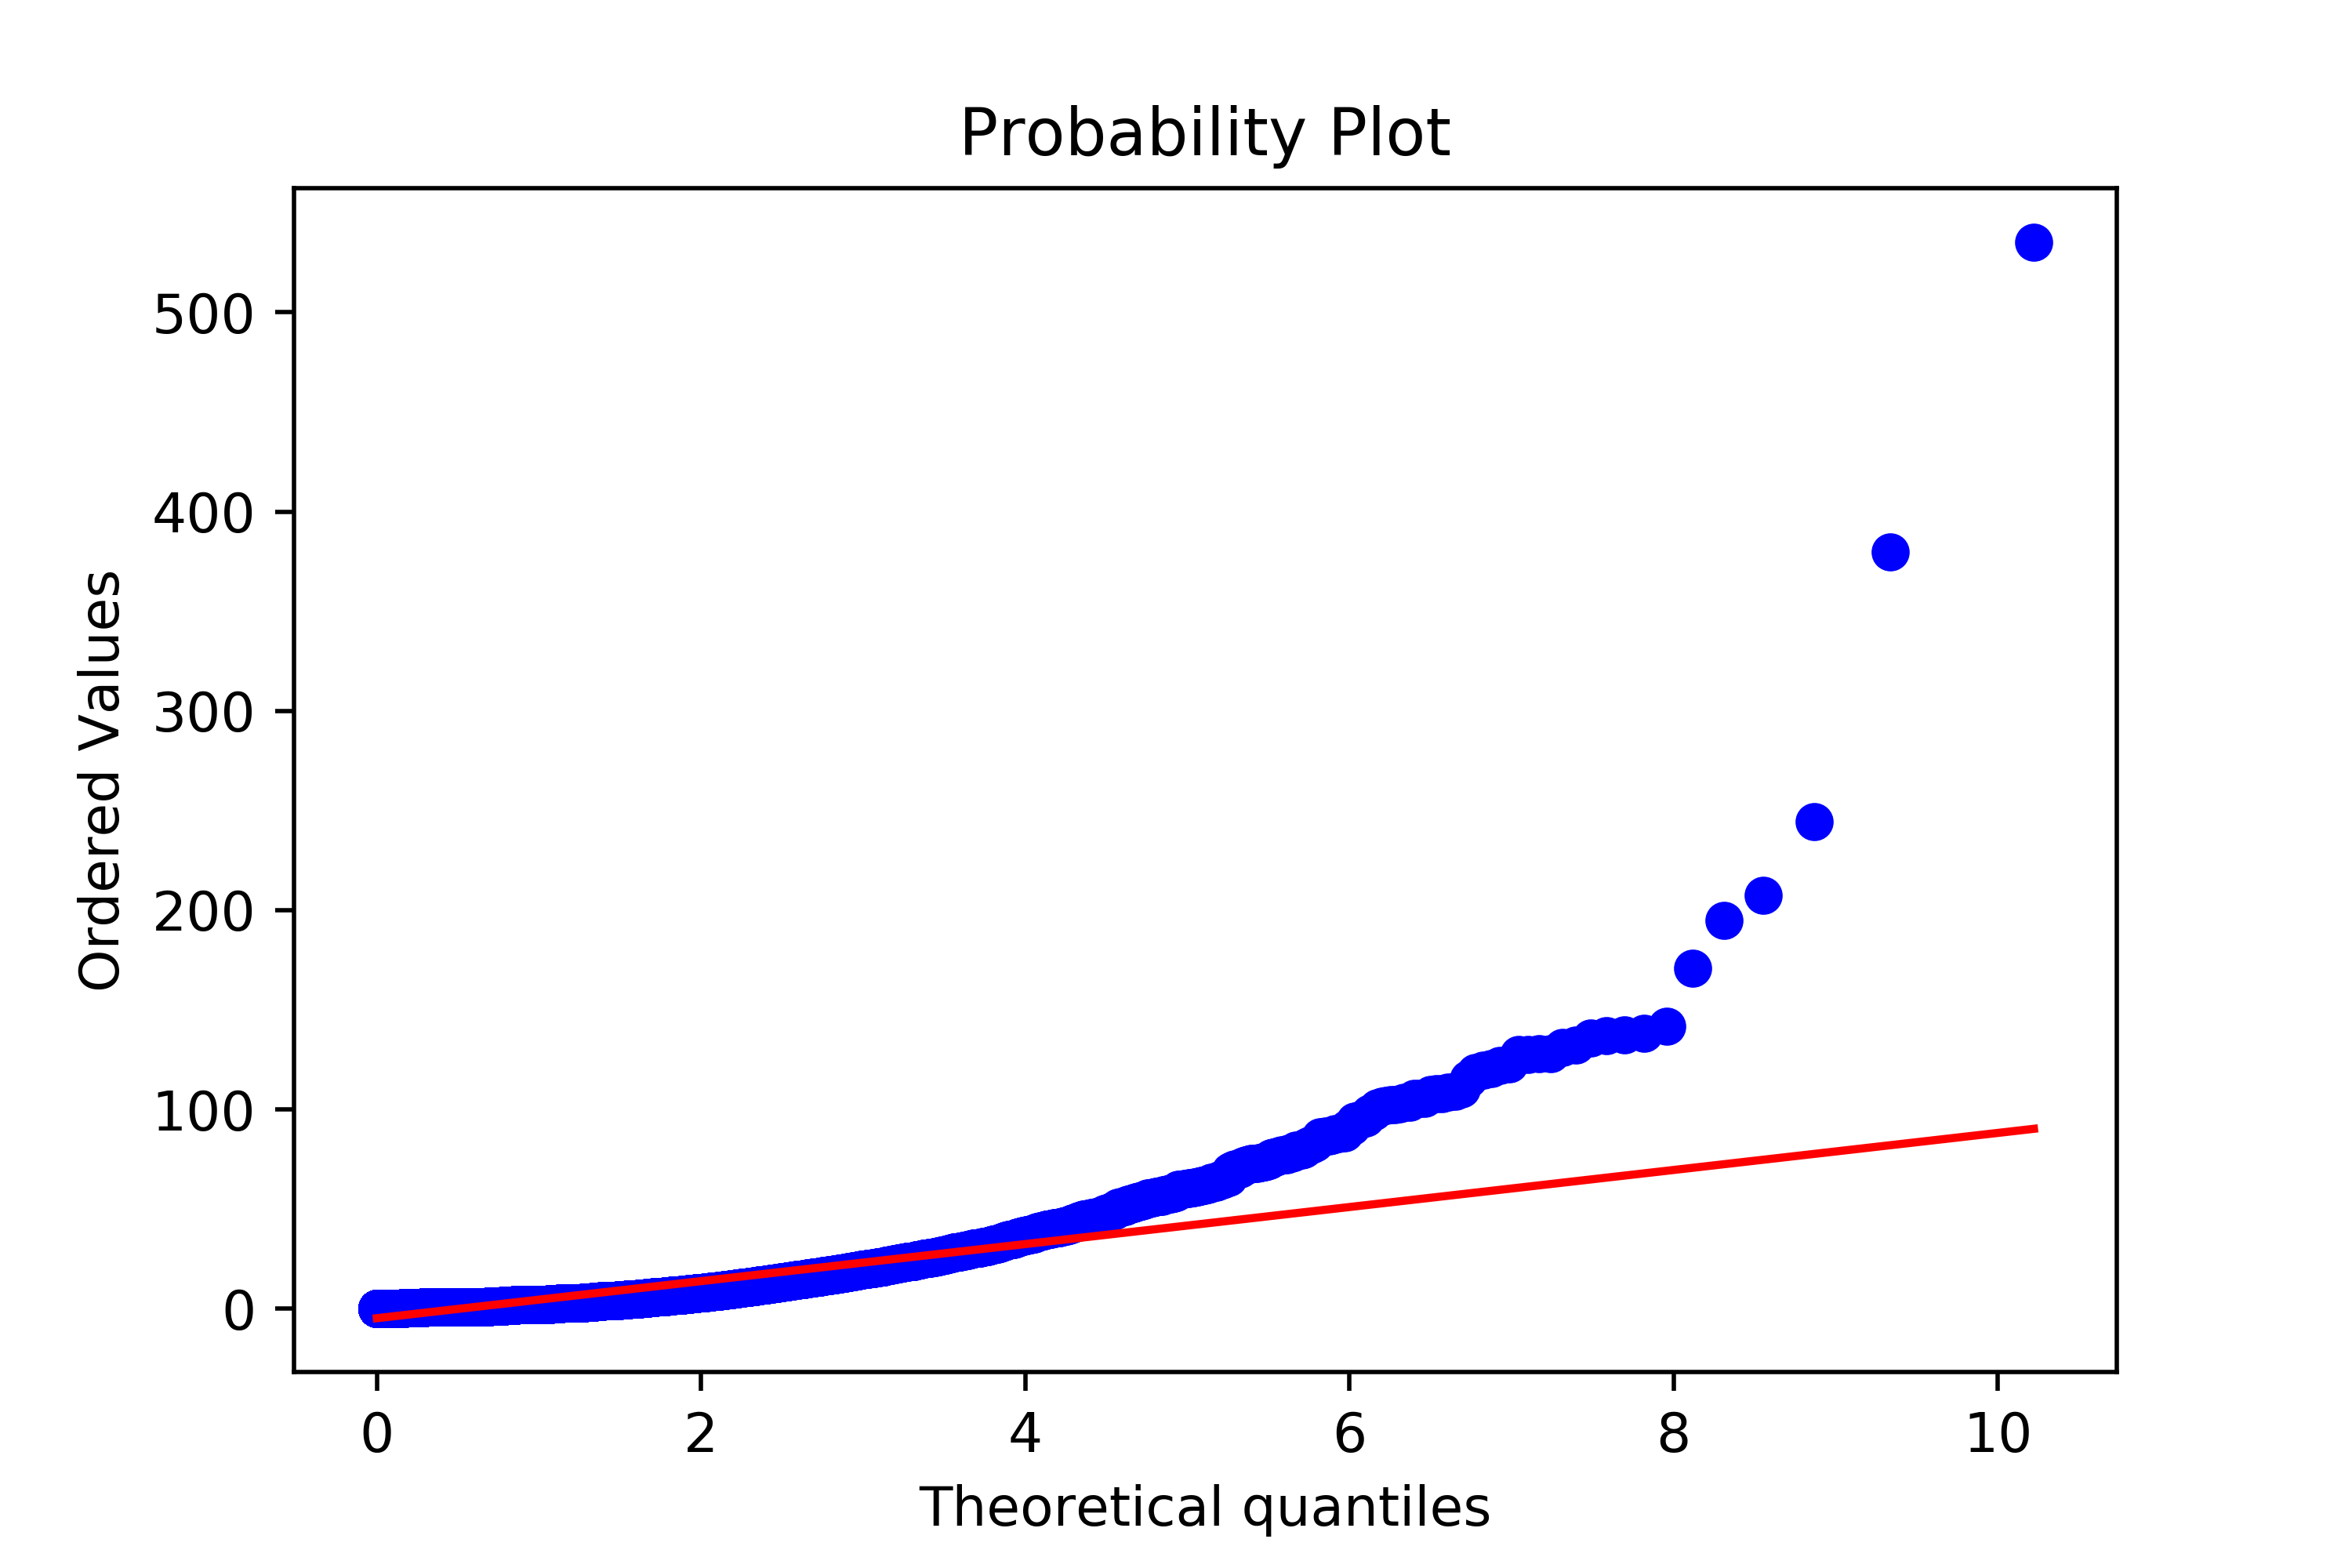
\includegraphics[width=60mm]{Figures/QQ_pos_k1.png}}
{}
&
\subf{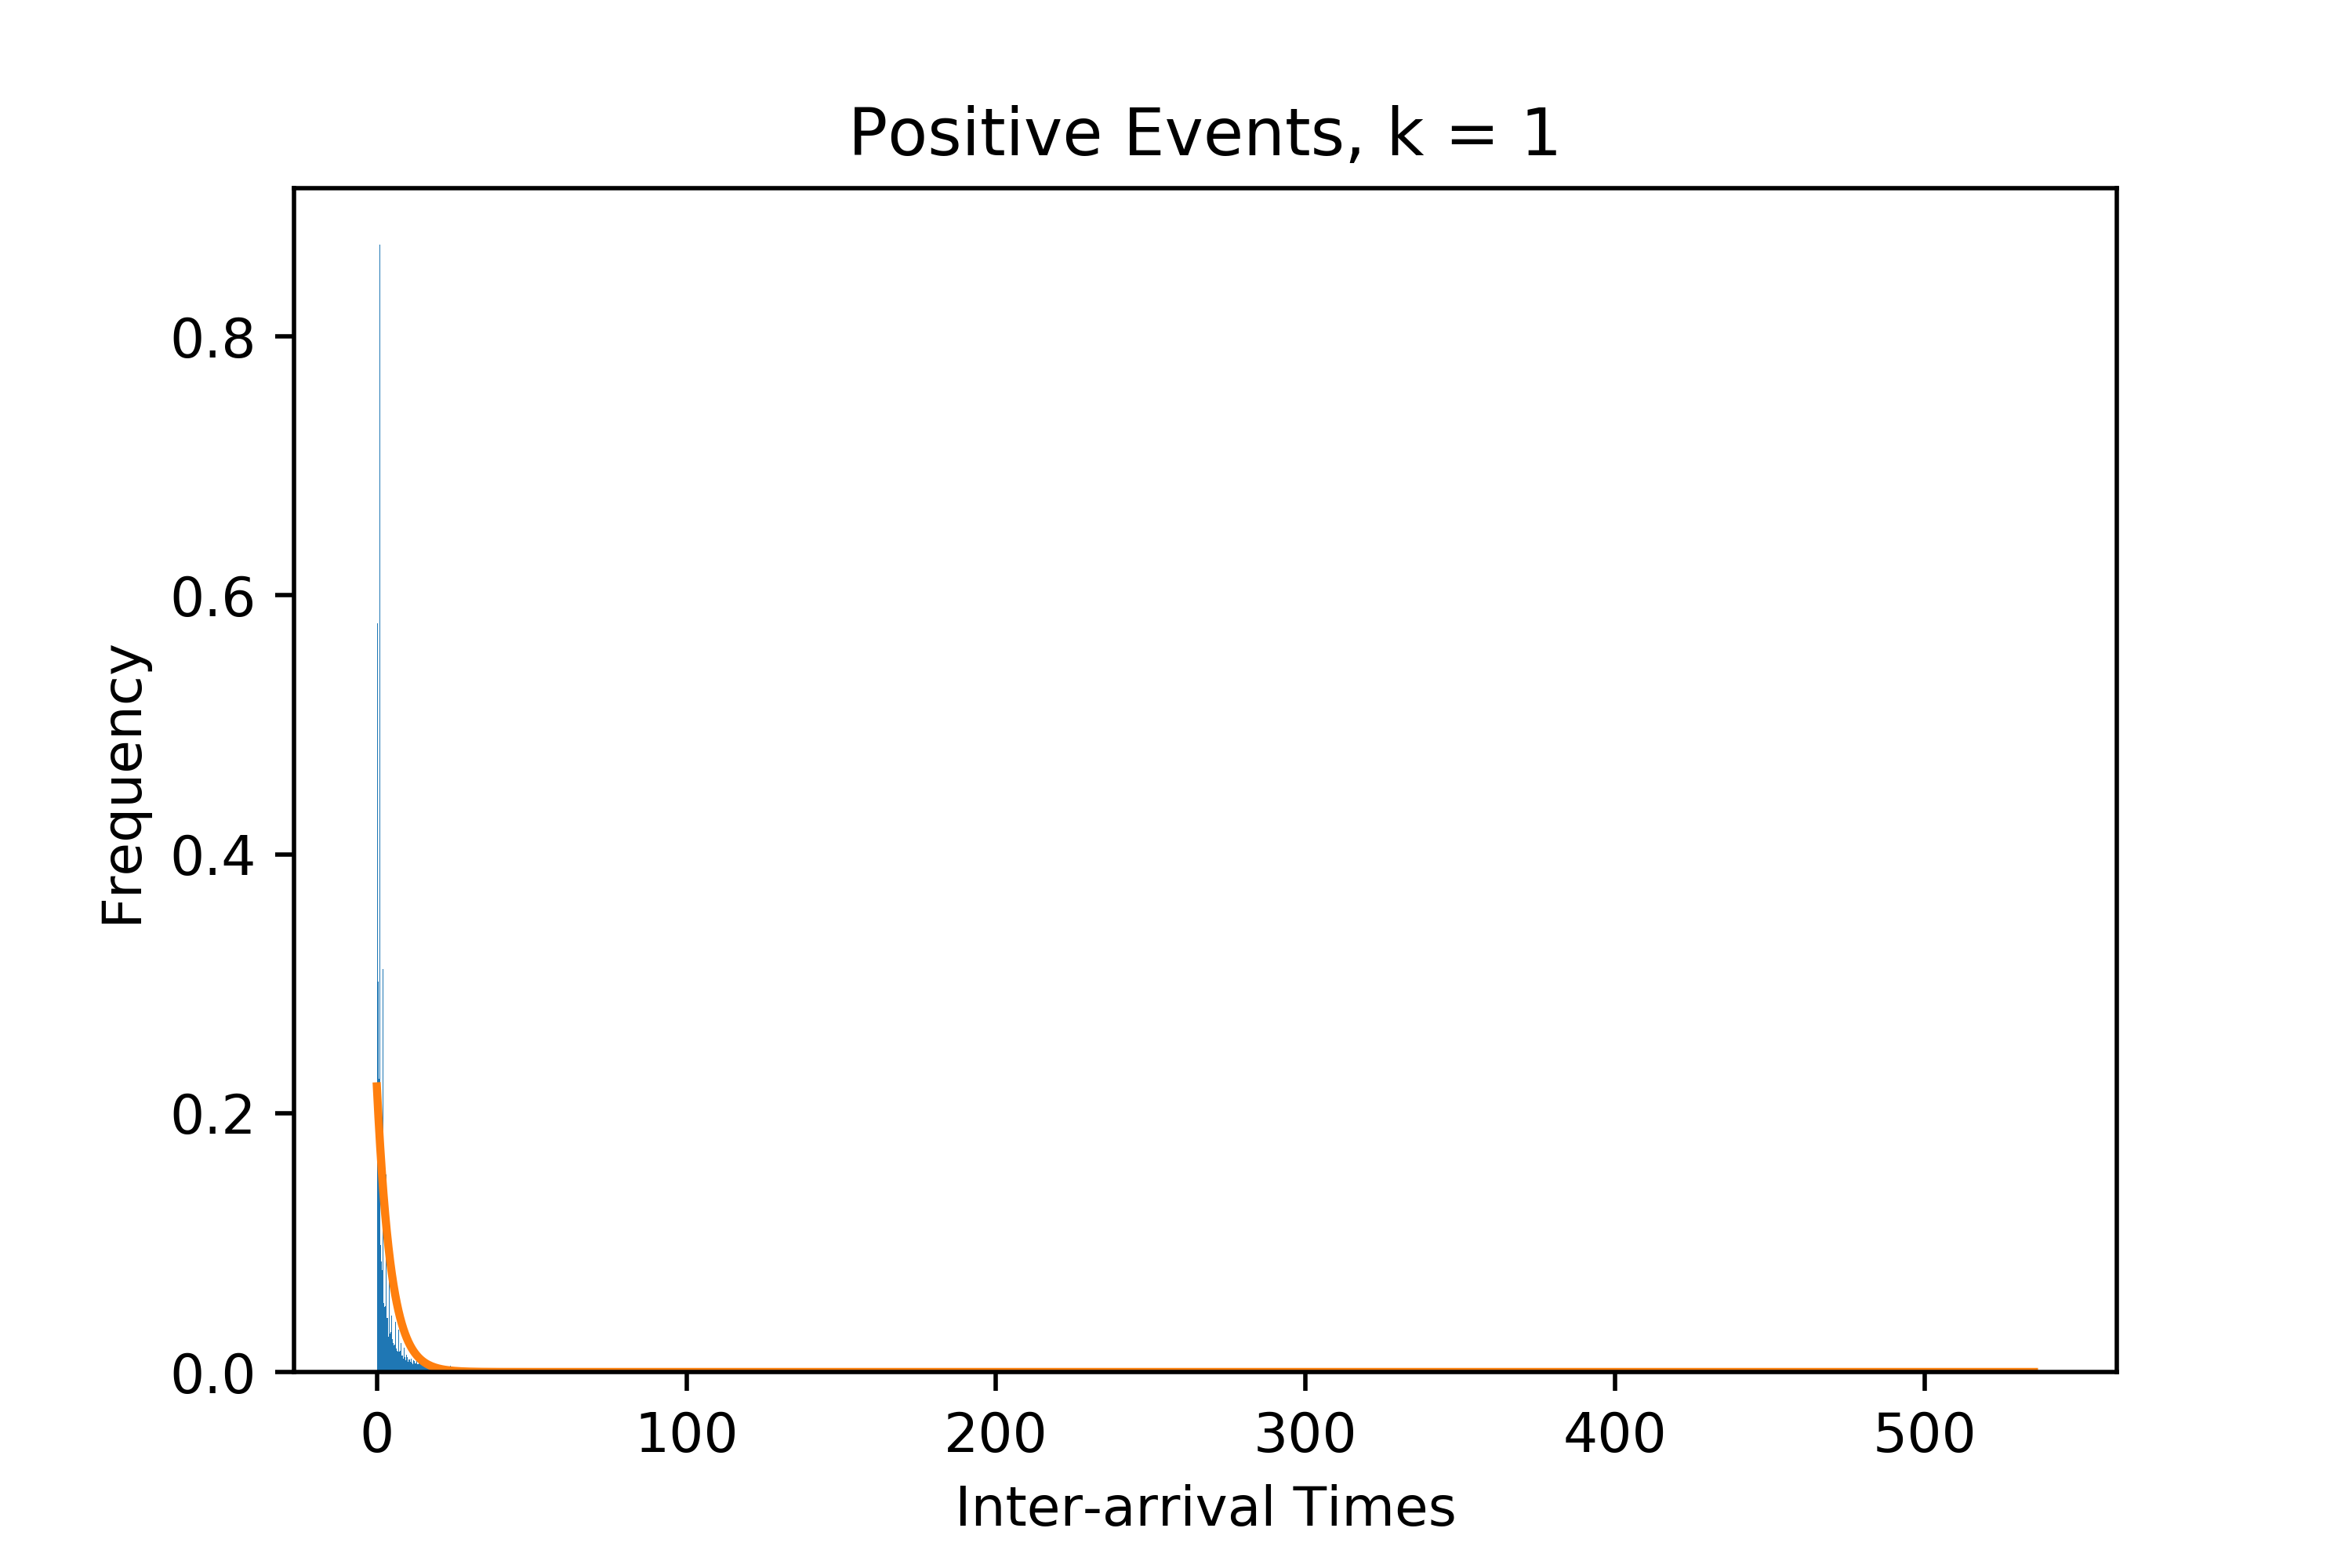
\includegraphics[width=60mm]{Figures/hist_pos_k1.png}}
{}
\\
\subf{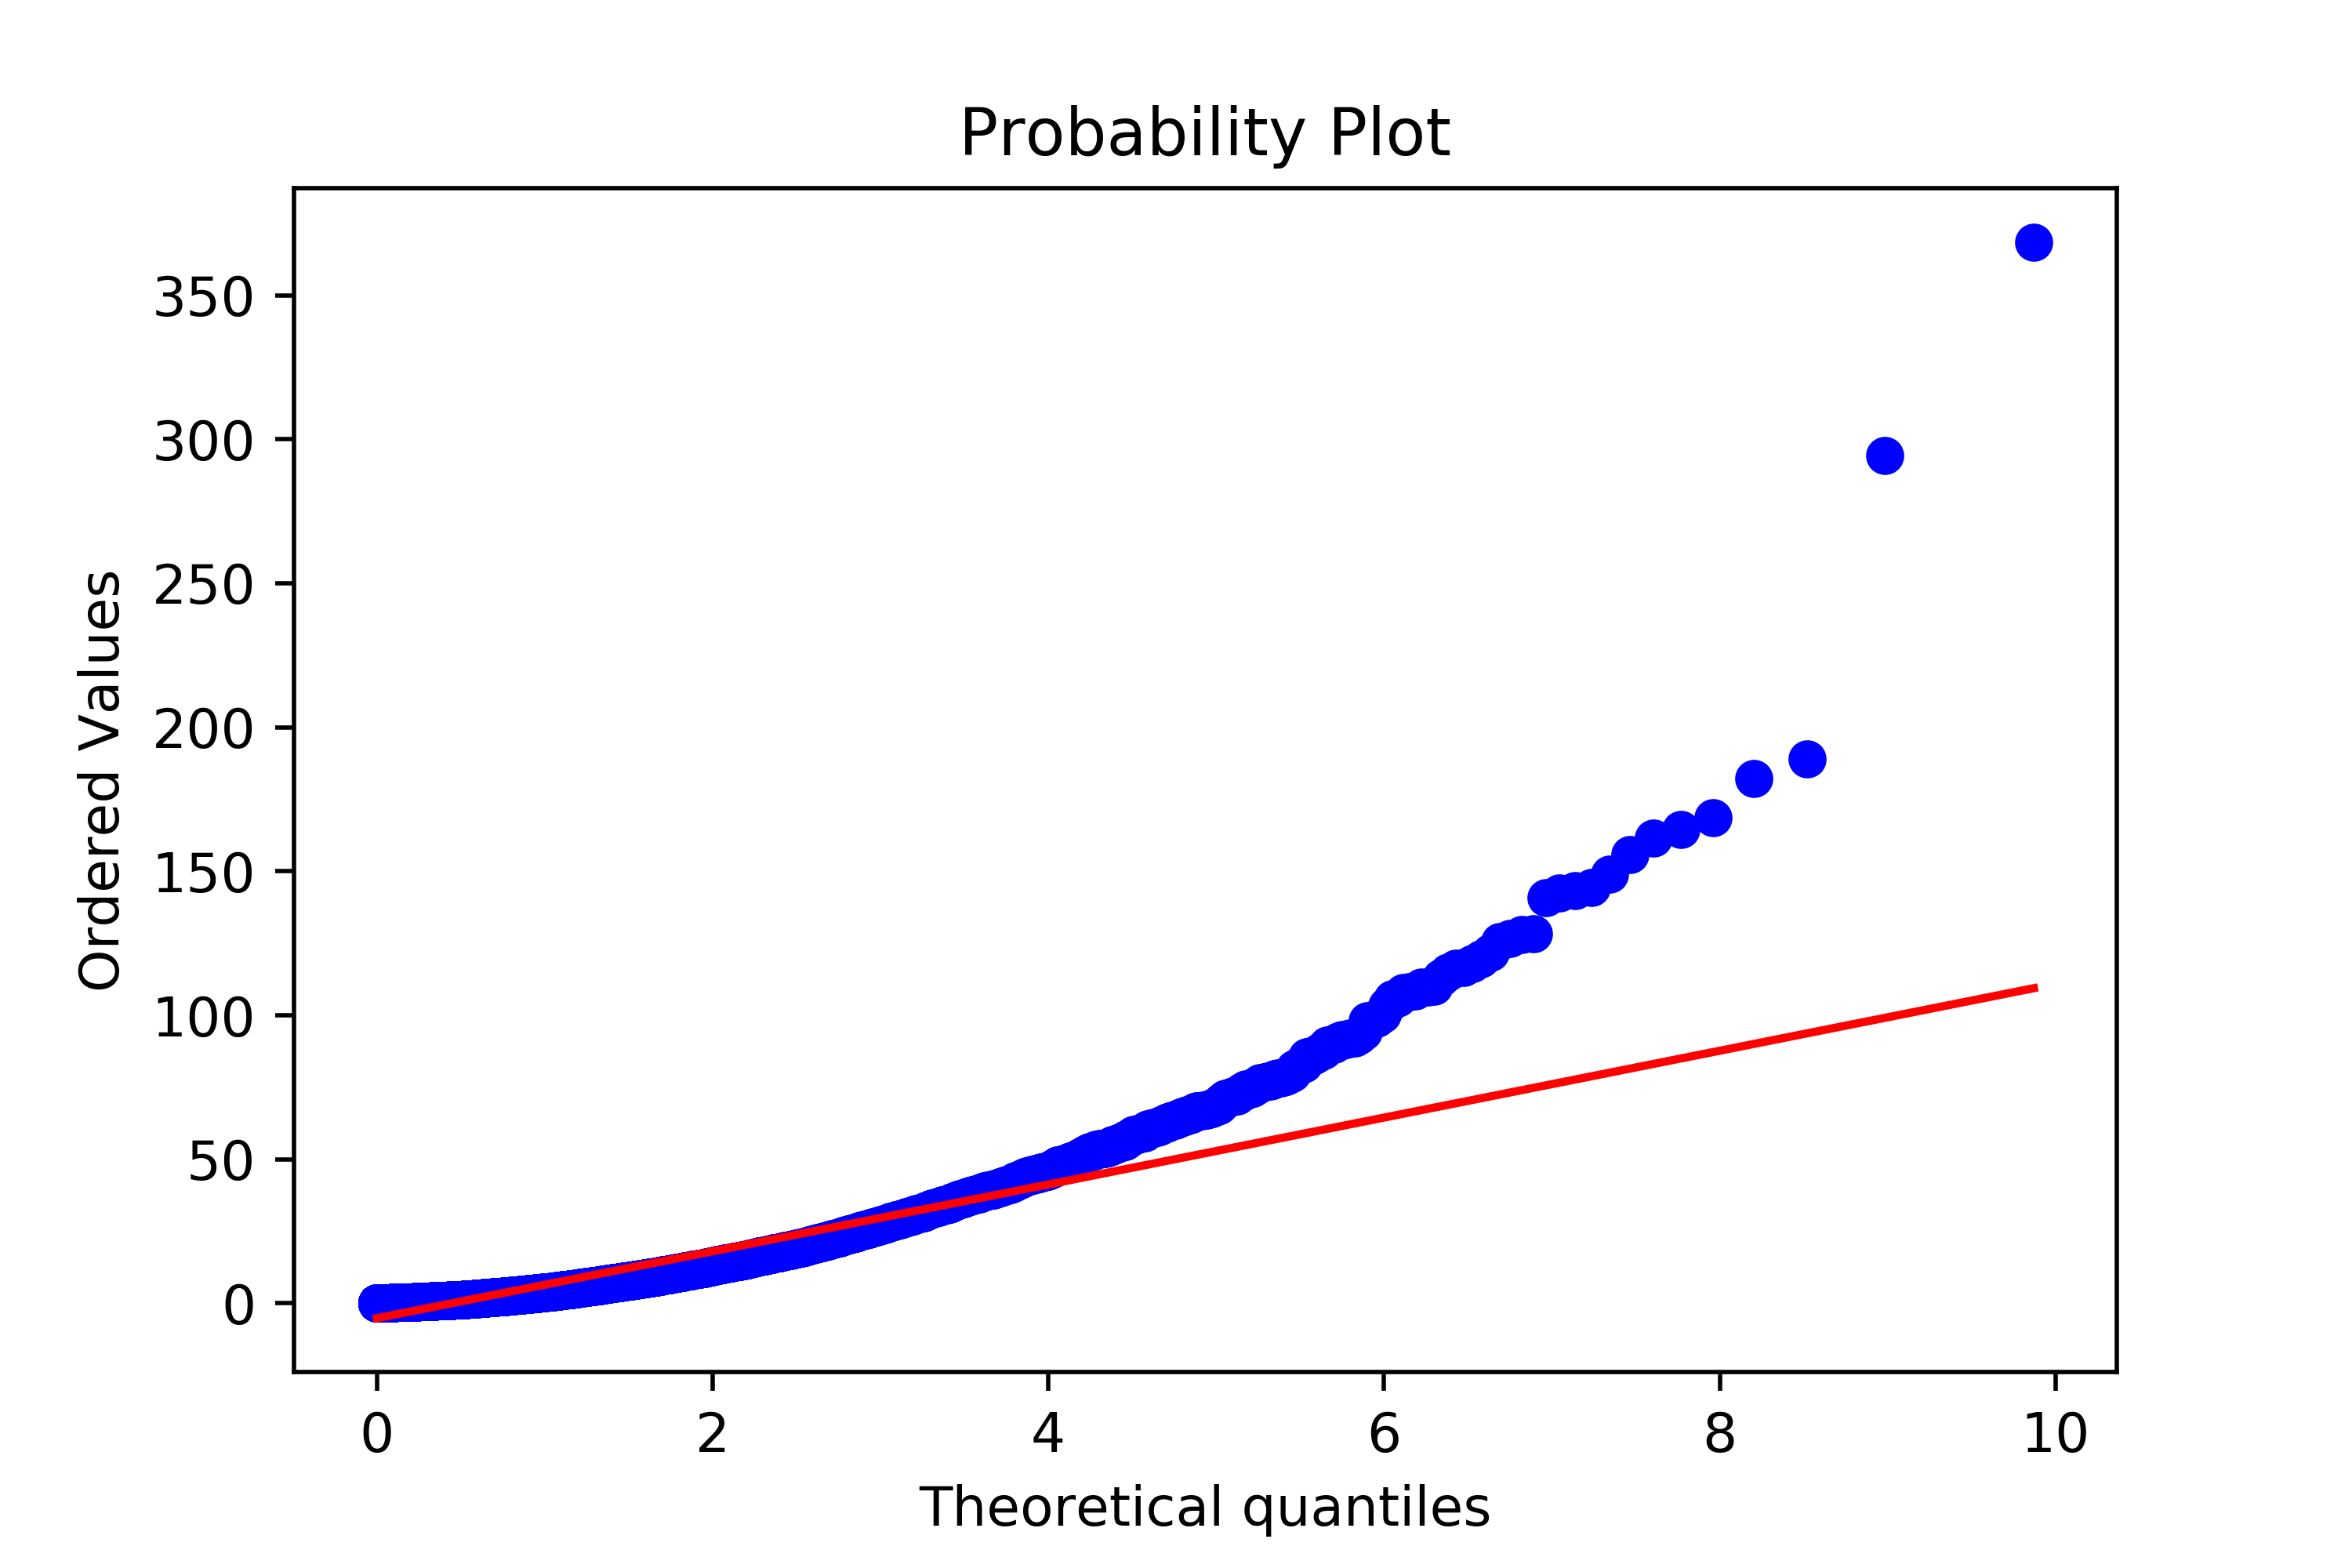
\includegraphics[width=60mm]{Figures/QQ_pos_k2.png}}
{}
&
\subf{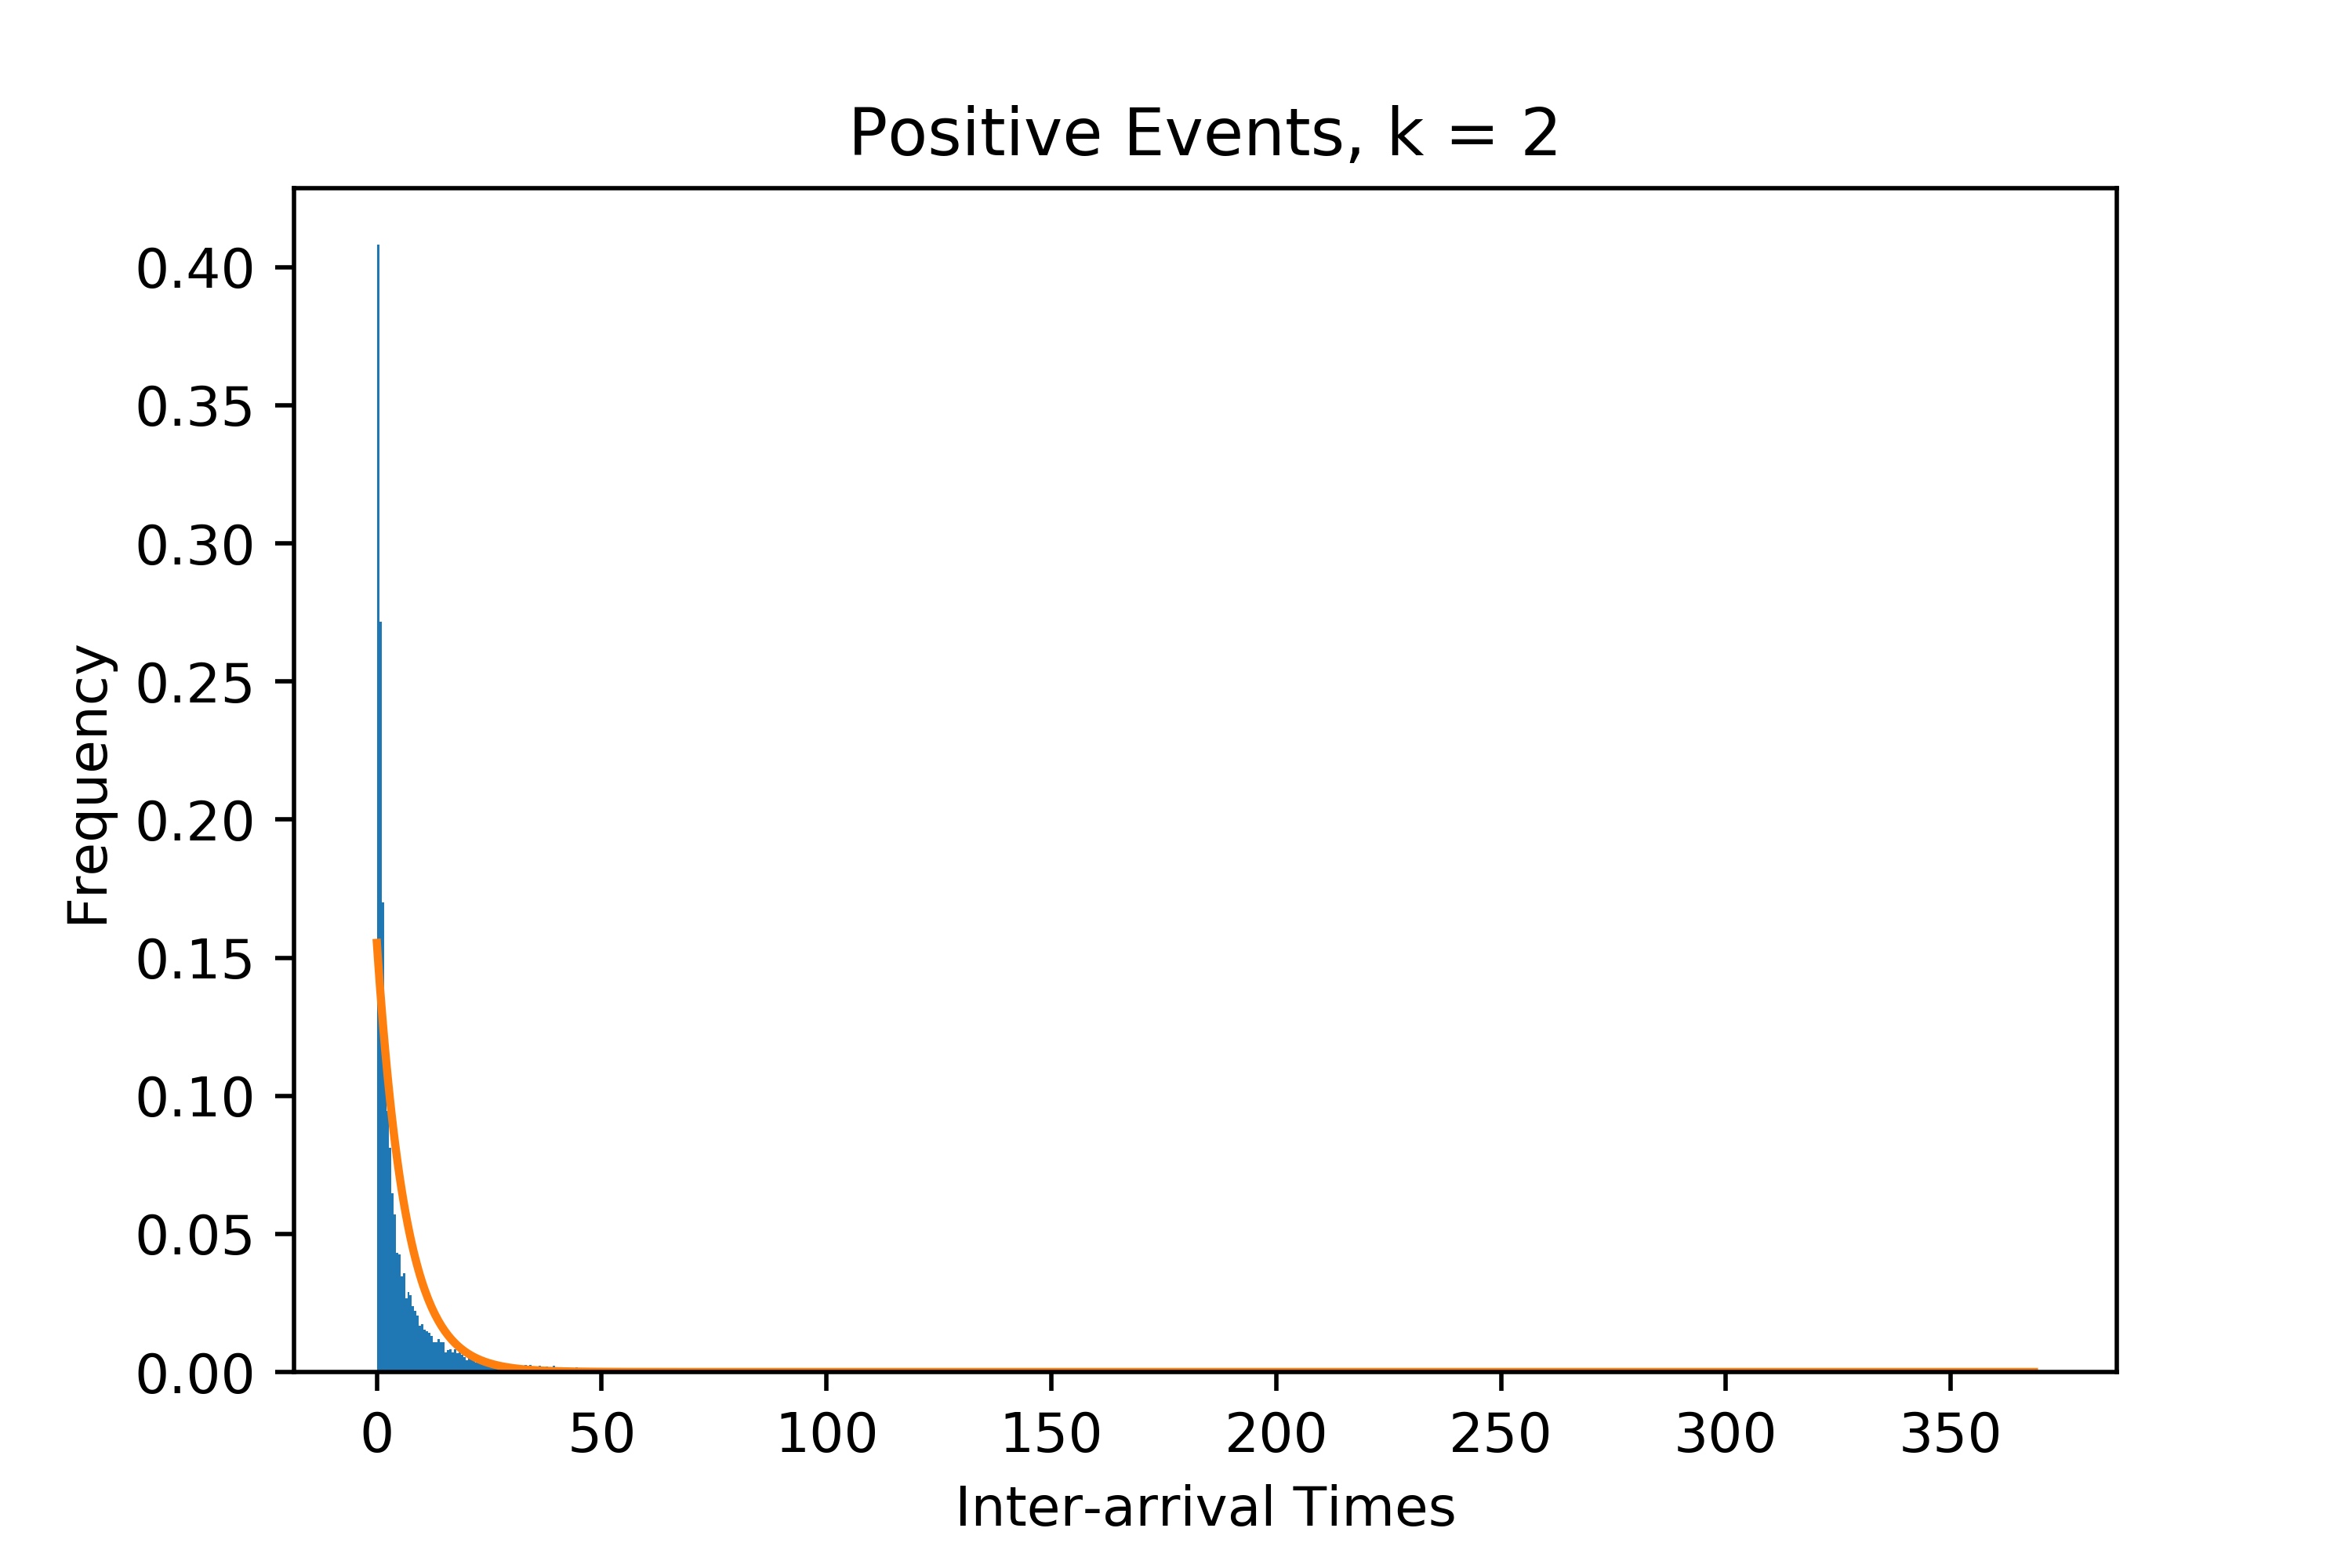
\includegraphics[width=60mm]{Figures/hist_pos_k2.png}}
{}
\\
\hline
\end{tabular}
\label{fig:interarrivals_pos}
\end{figure}

\begin{figure}
\centering
\caption{Inter-Arrival Times for Negative Events Compared to Exponential Distribution using Data from December 30, 2018}
\begin{tabular}{cc}
\hline
\subf{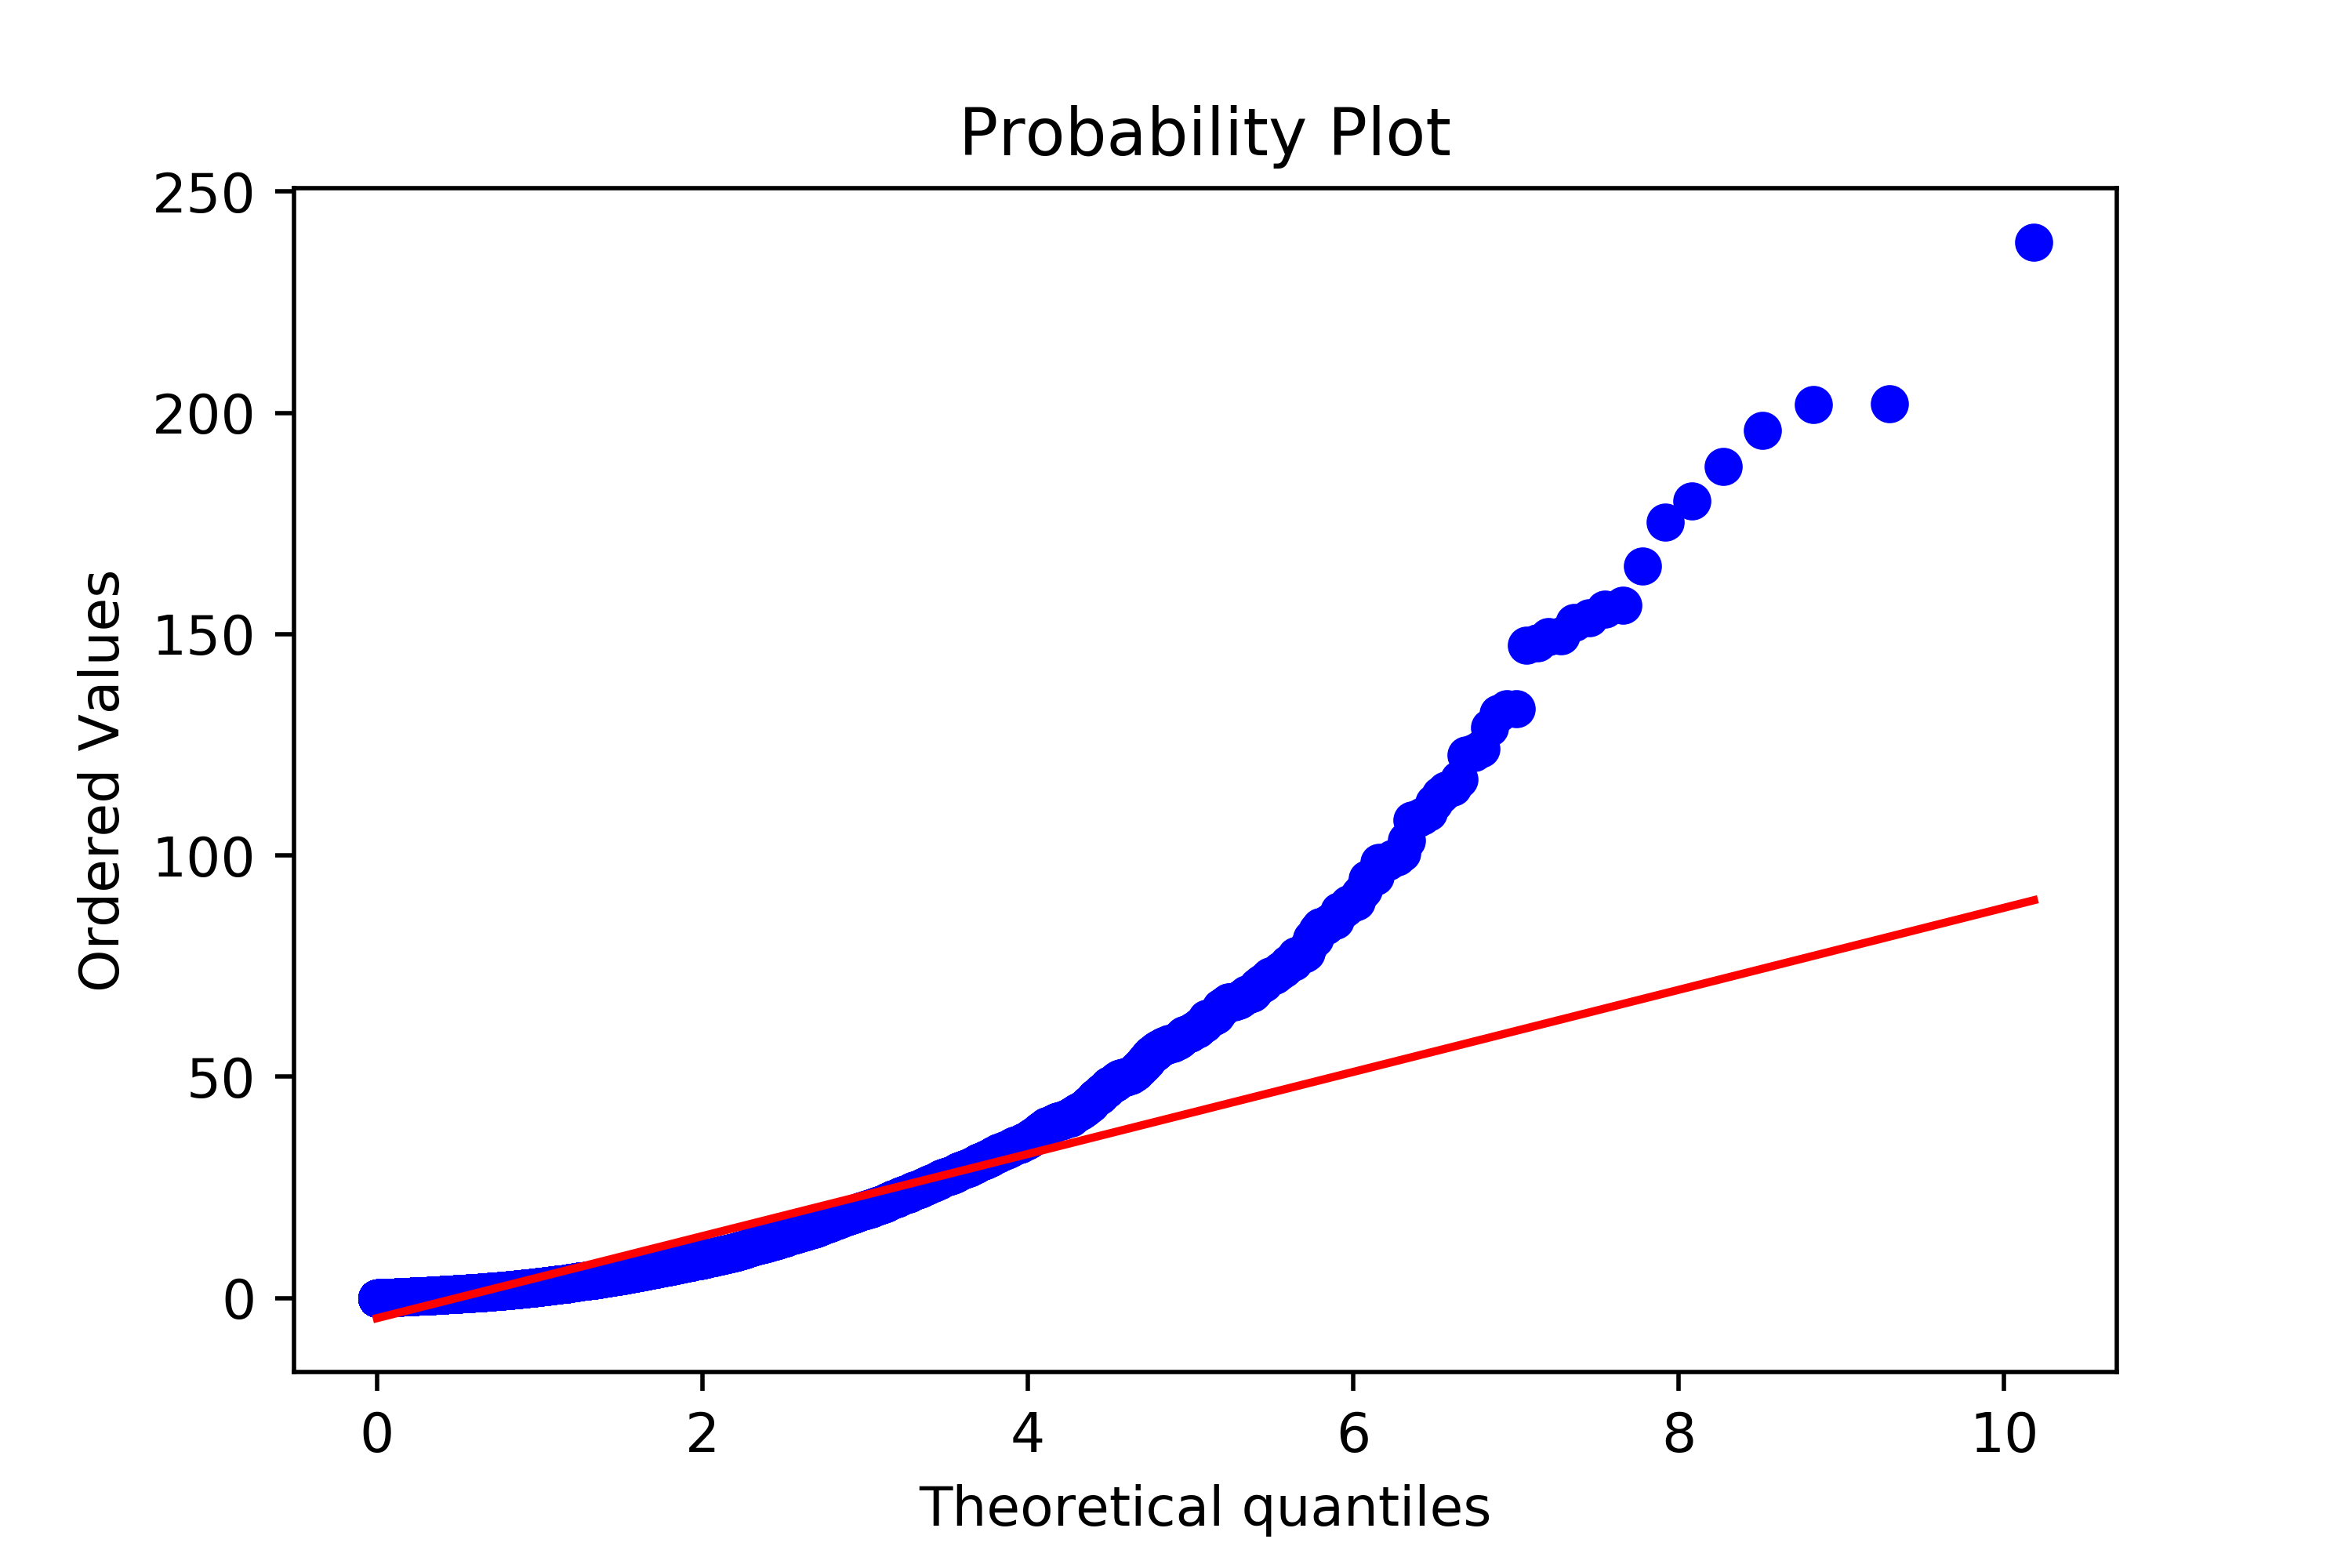
\includegraphics[width=60mm]{Figures/QQ_neg_k-2.png}}
{}
&
\subf{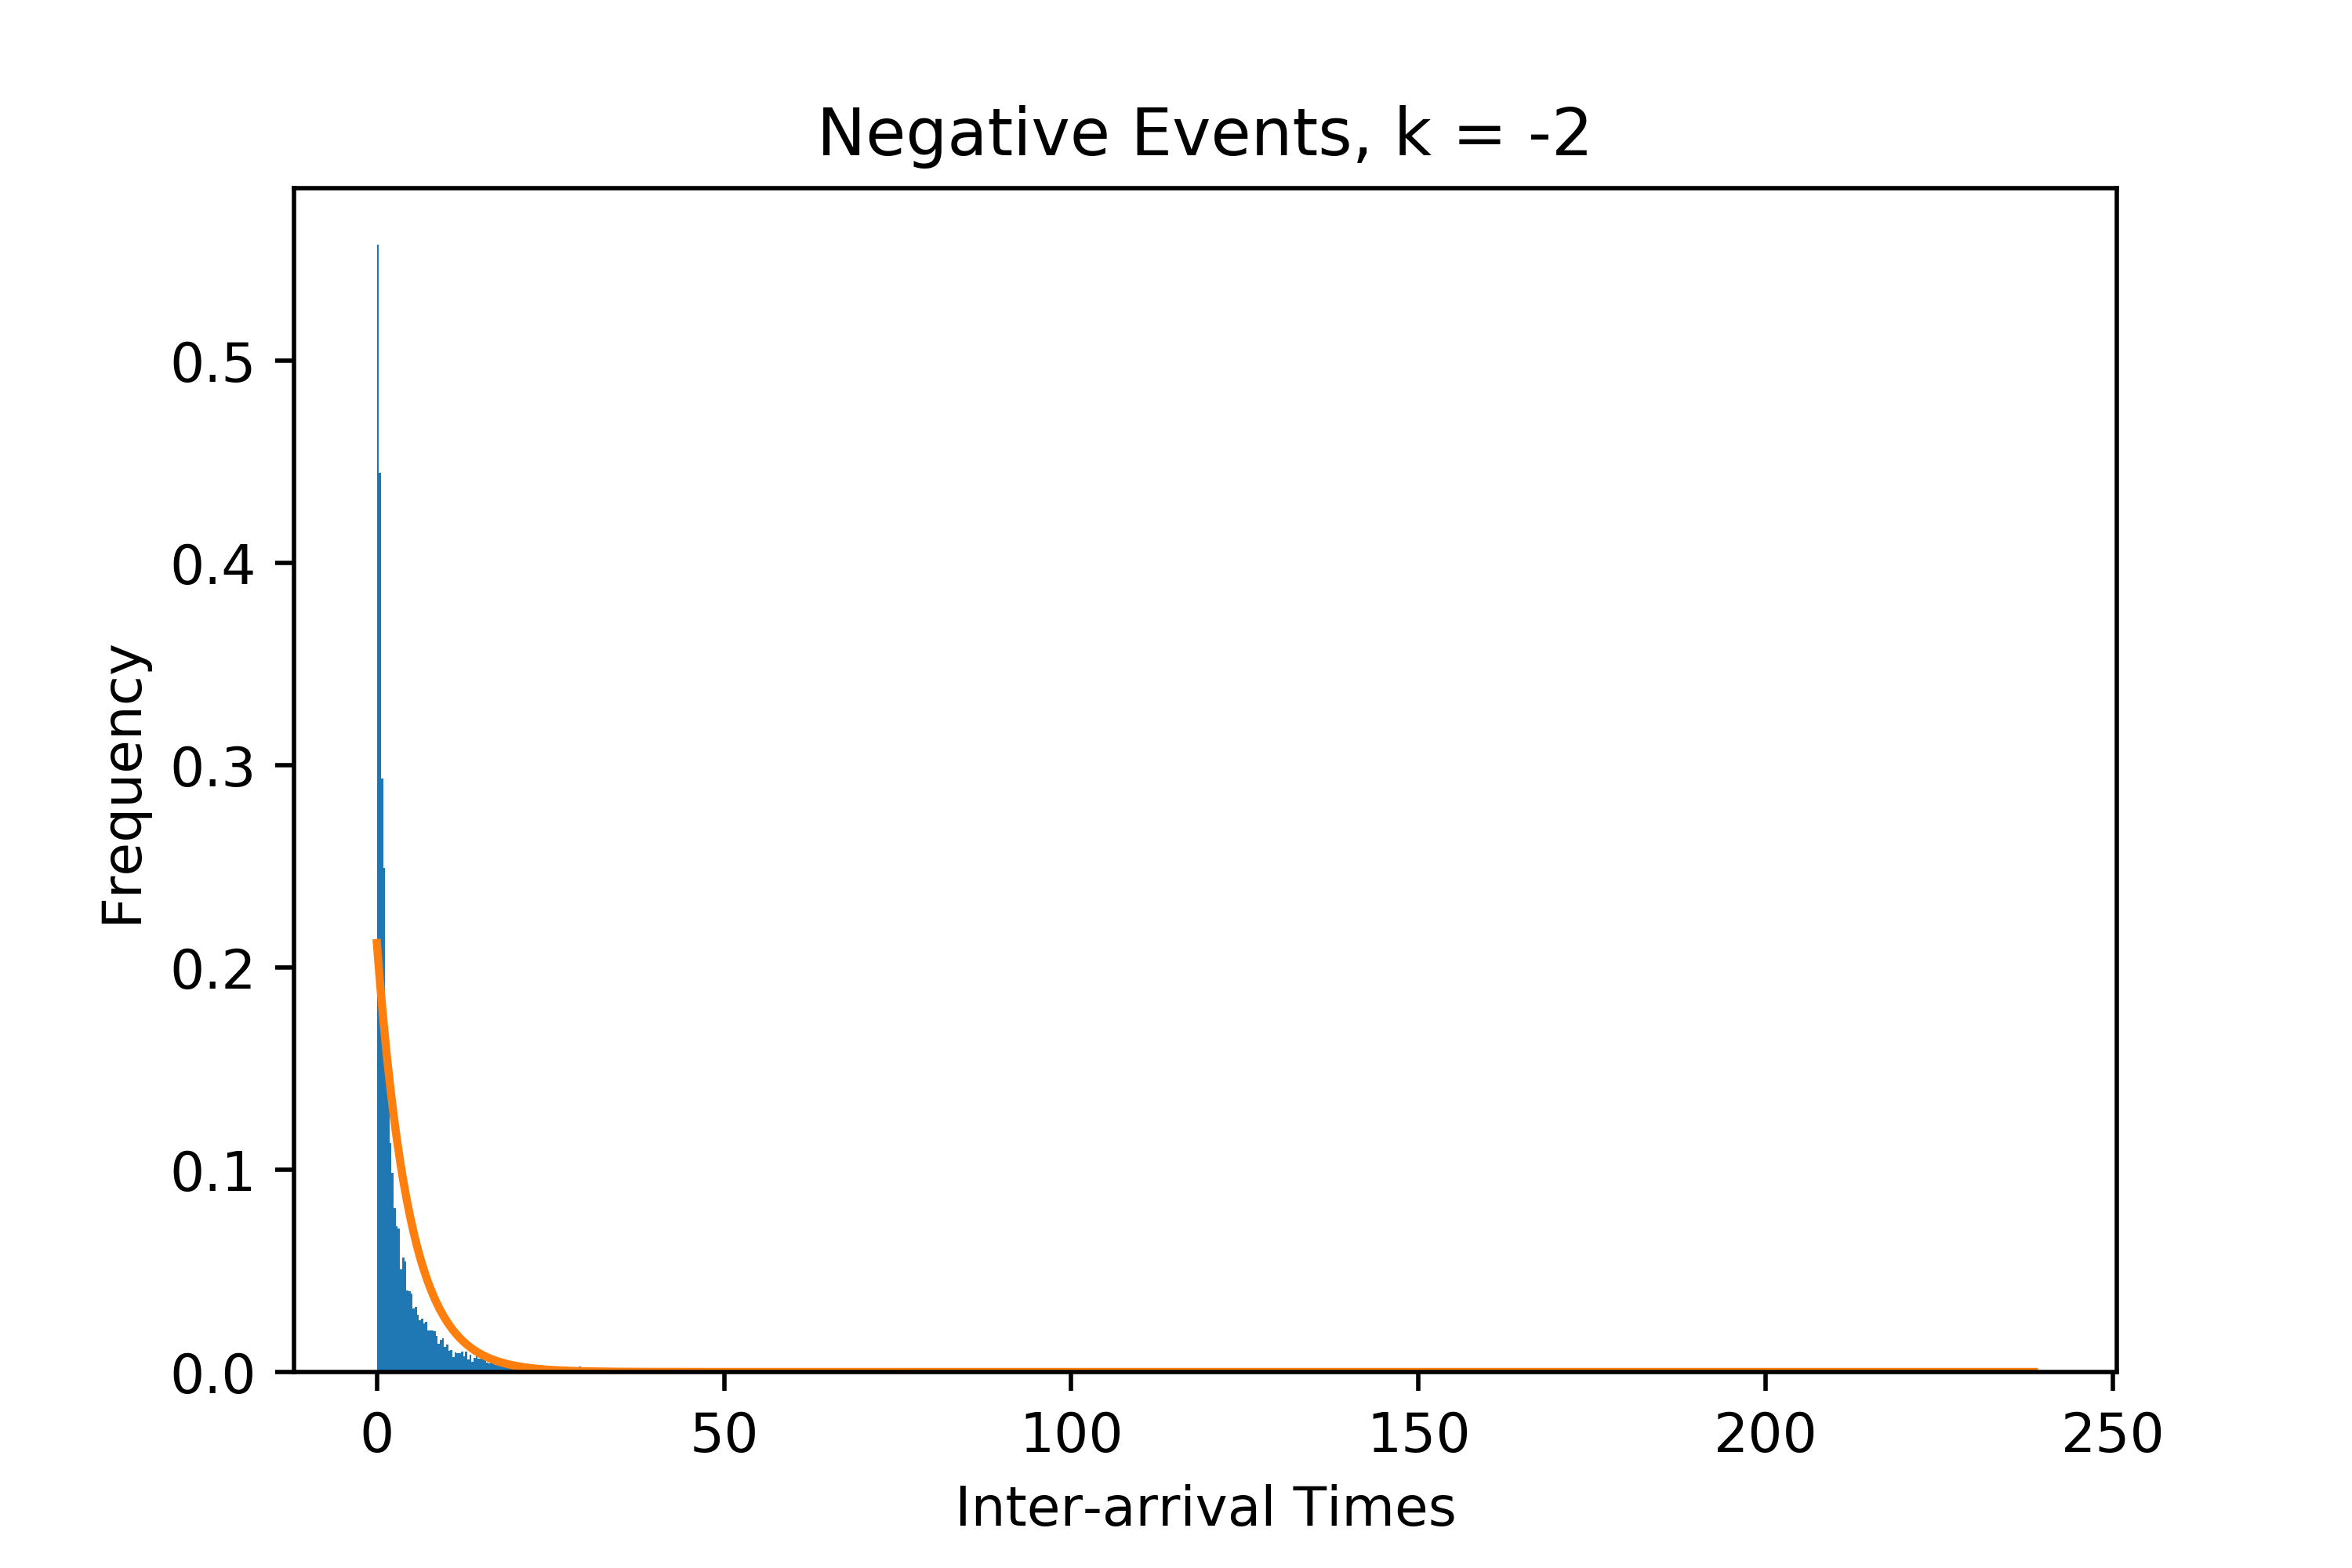
\includegraphics[width=60mm]{Figures/hist_neg_k-2.png}}
{}
\\
\subf{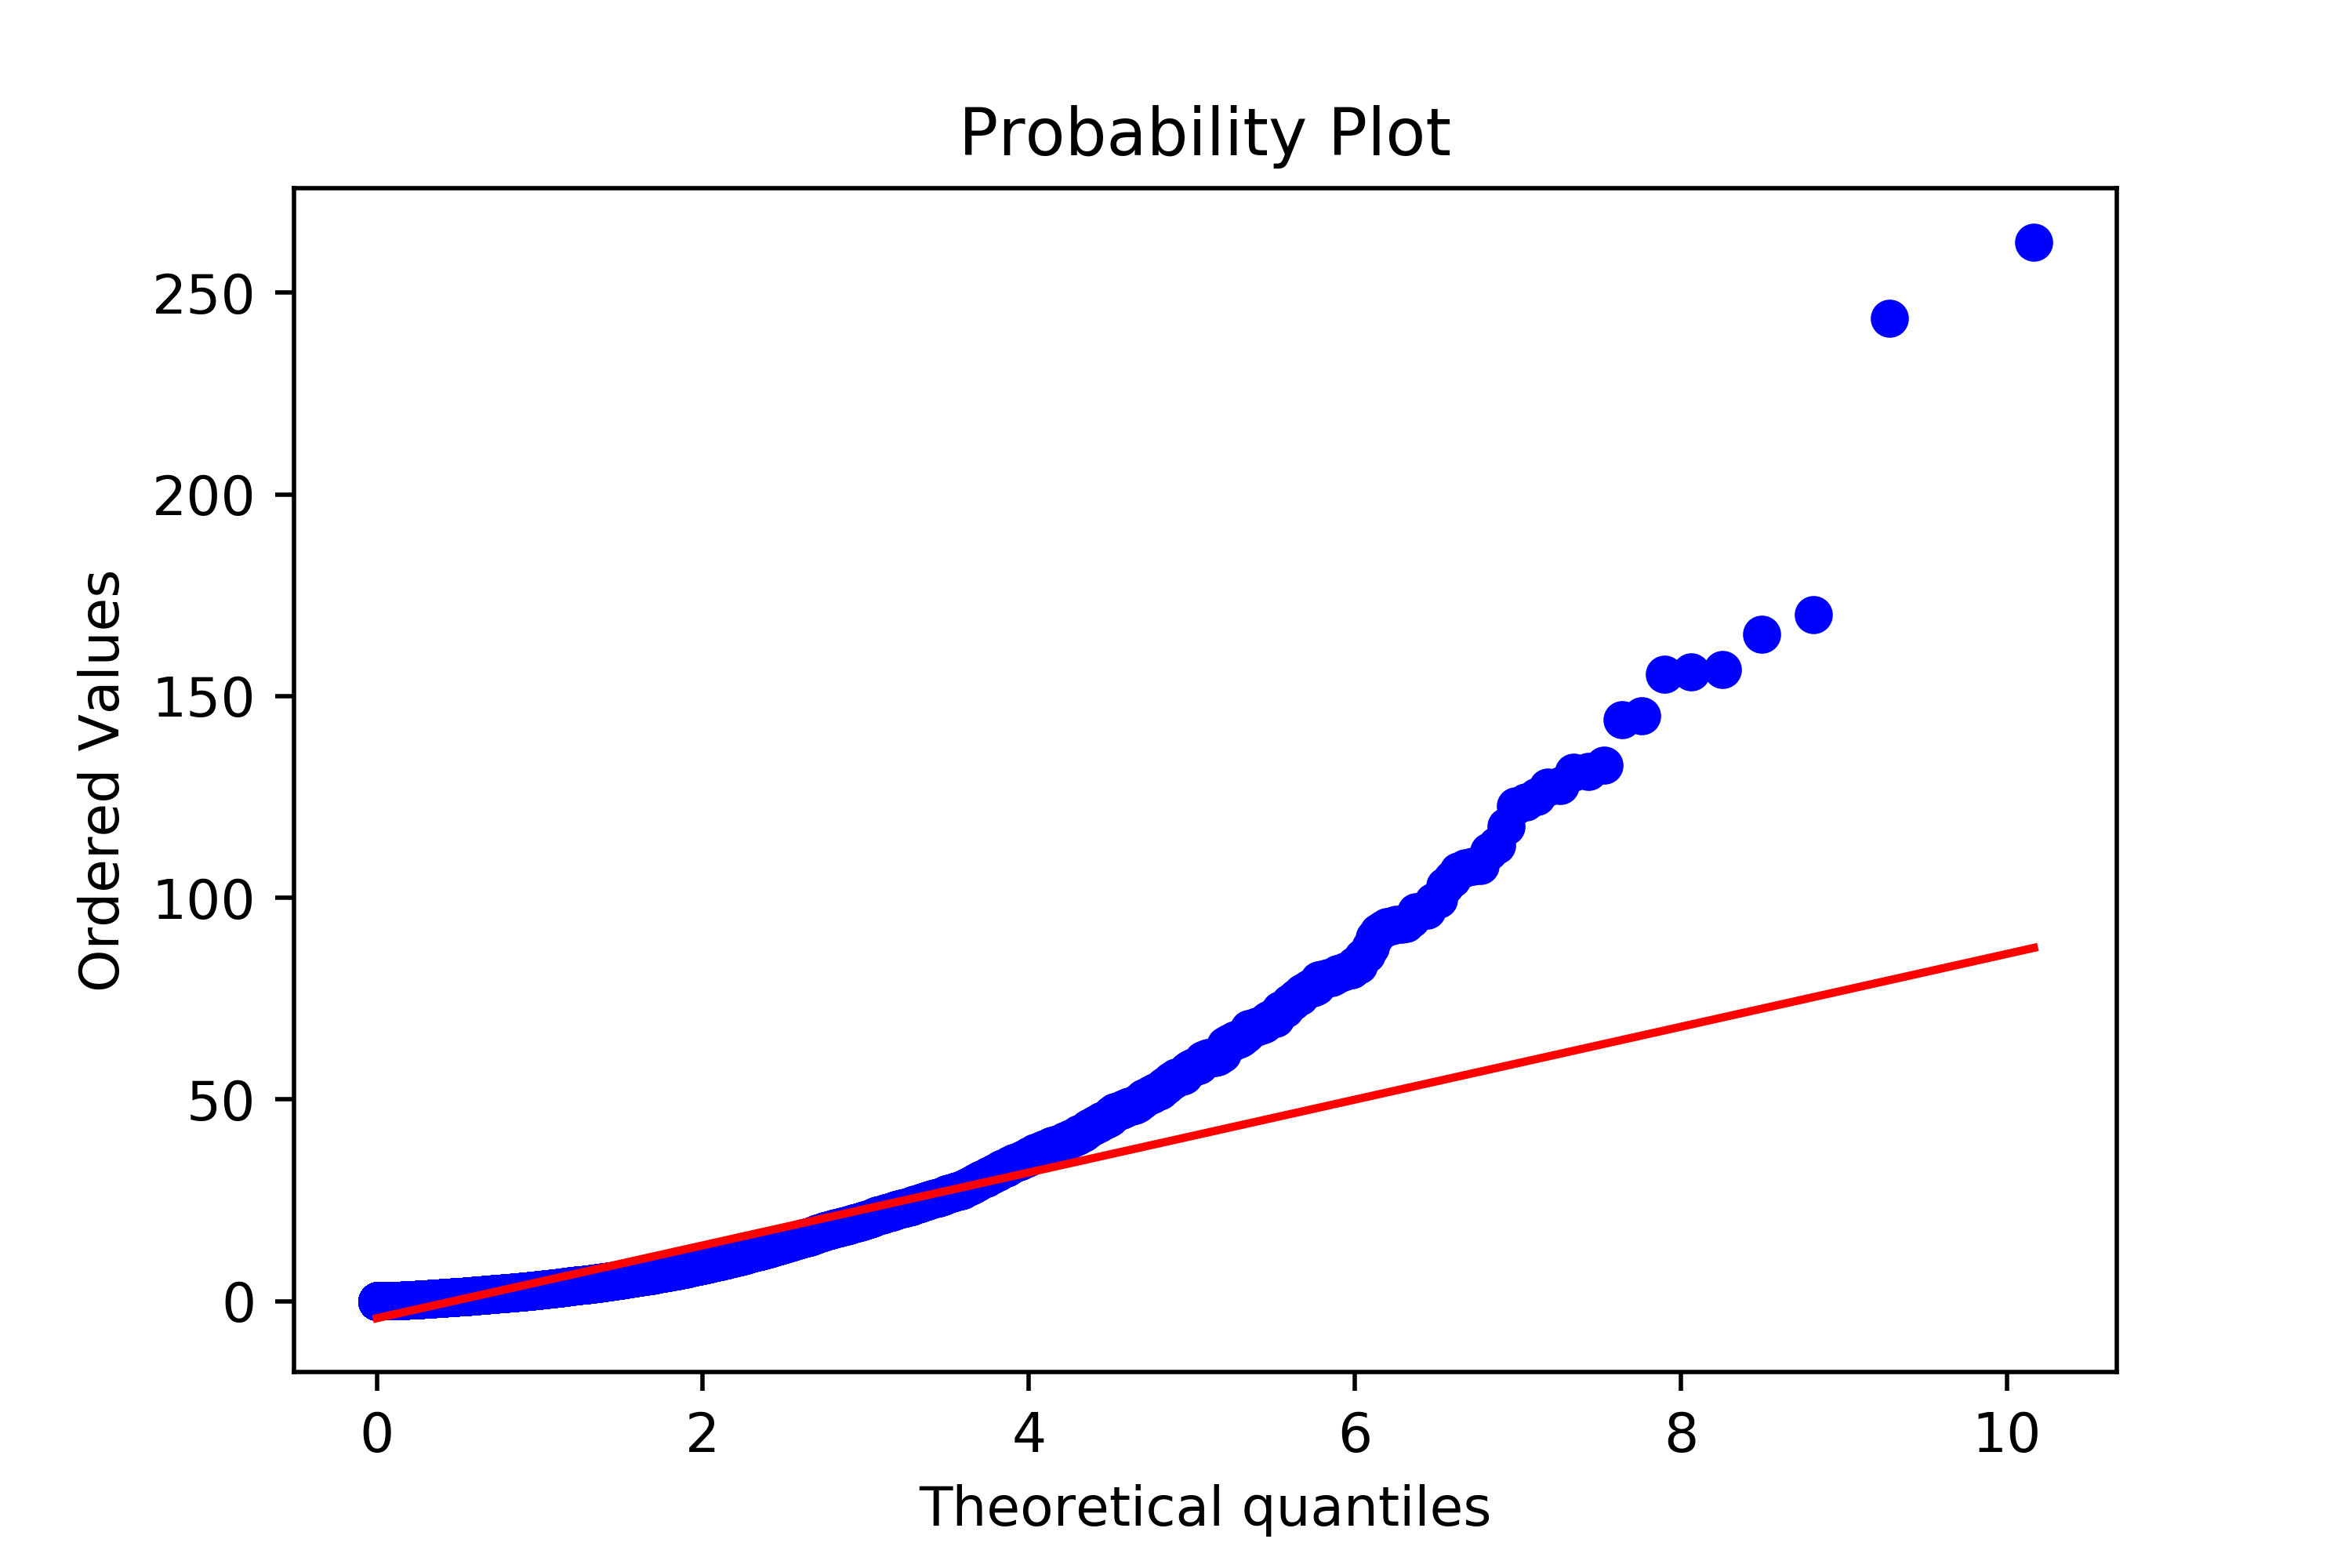
\includegraphics[width=60mm]{Figures/QQ_neg_k-1.png}}
{}
&
\subf{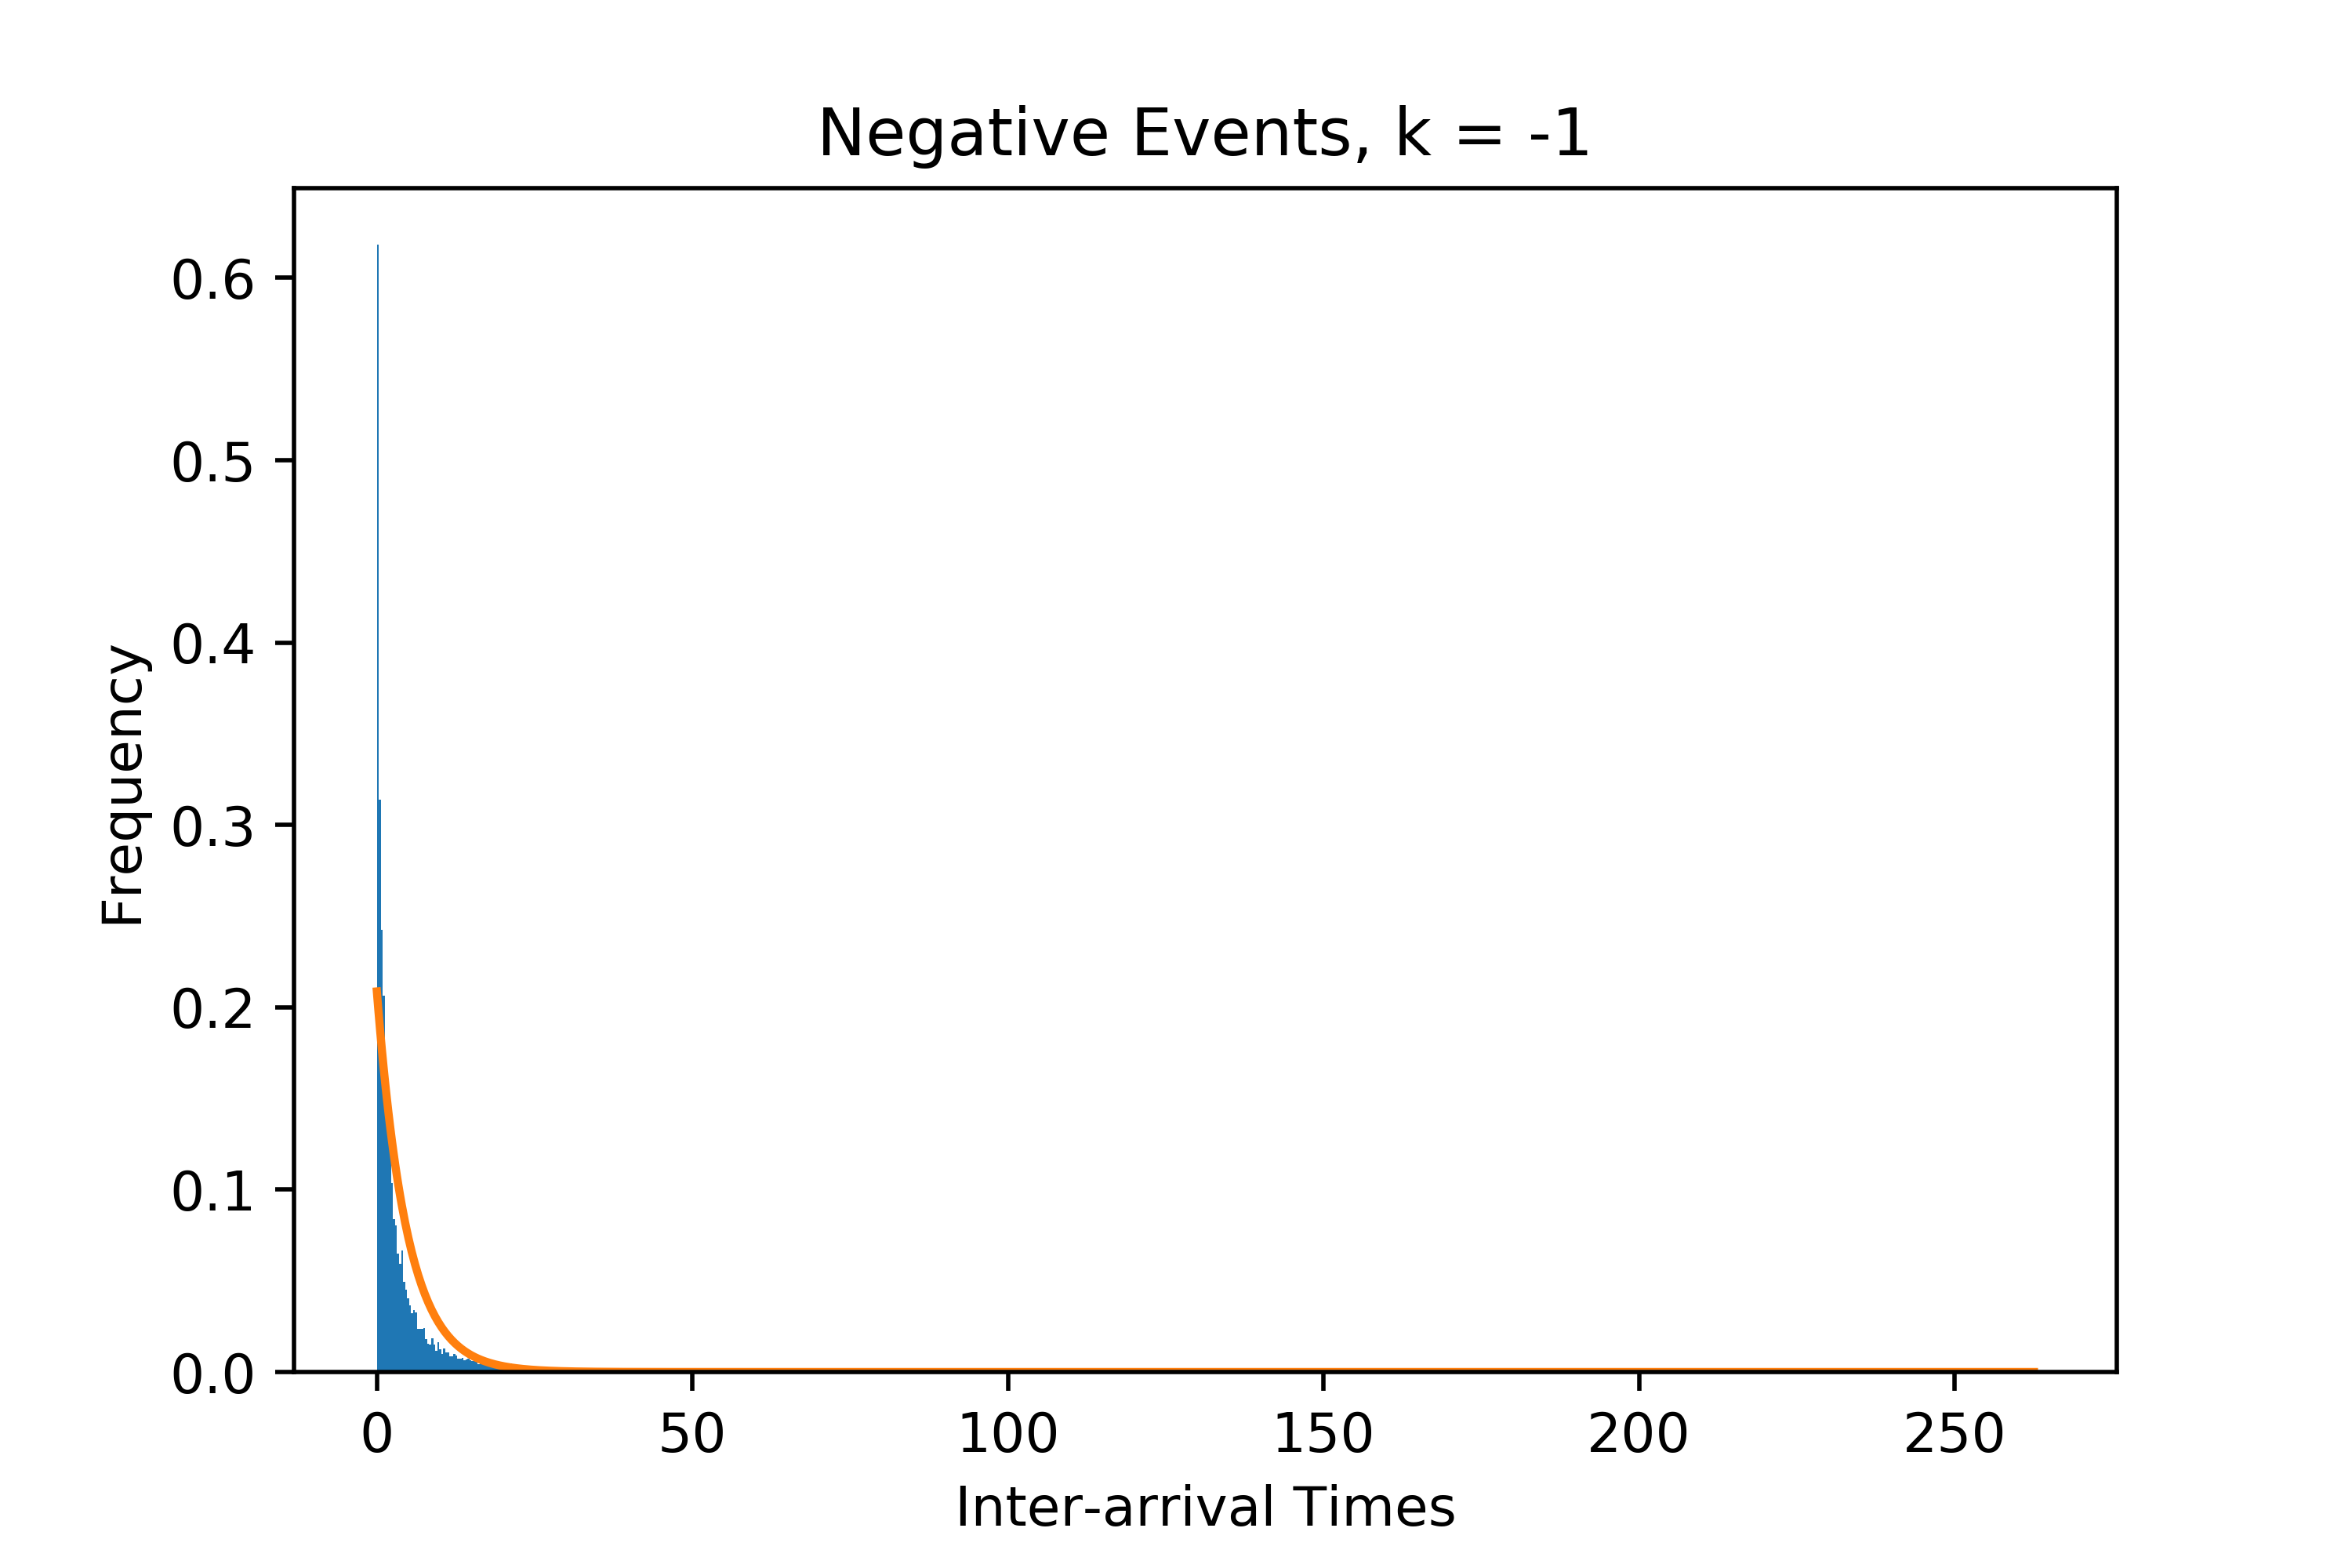
\includegraphics[width=60mm]{Figures/hist_neg_k-1.png}}
{}
\\
\subf{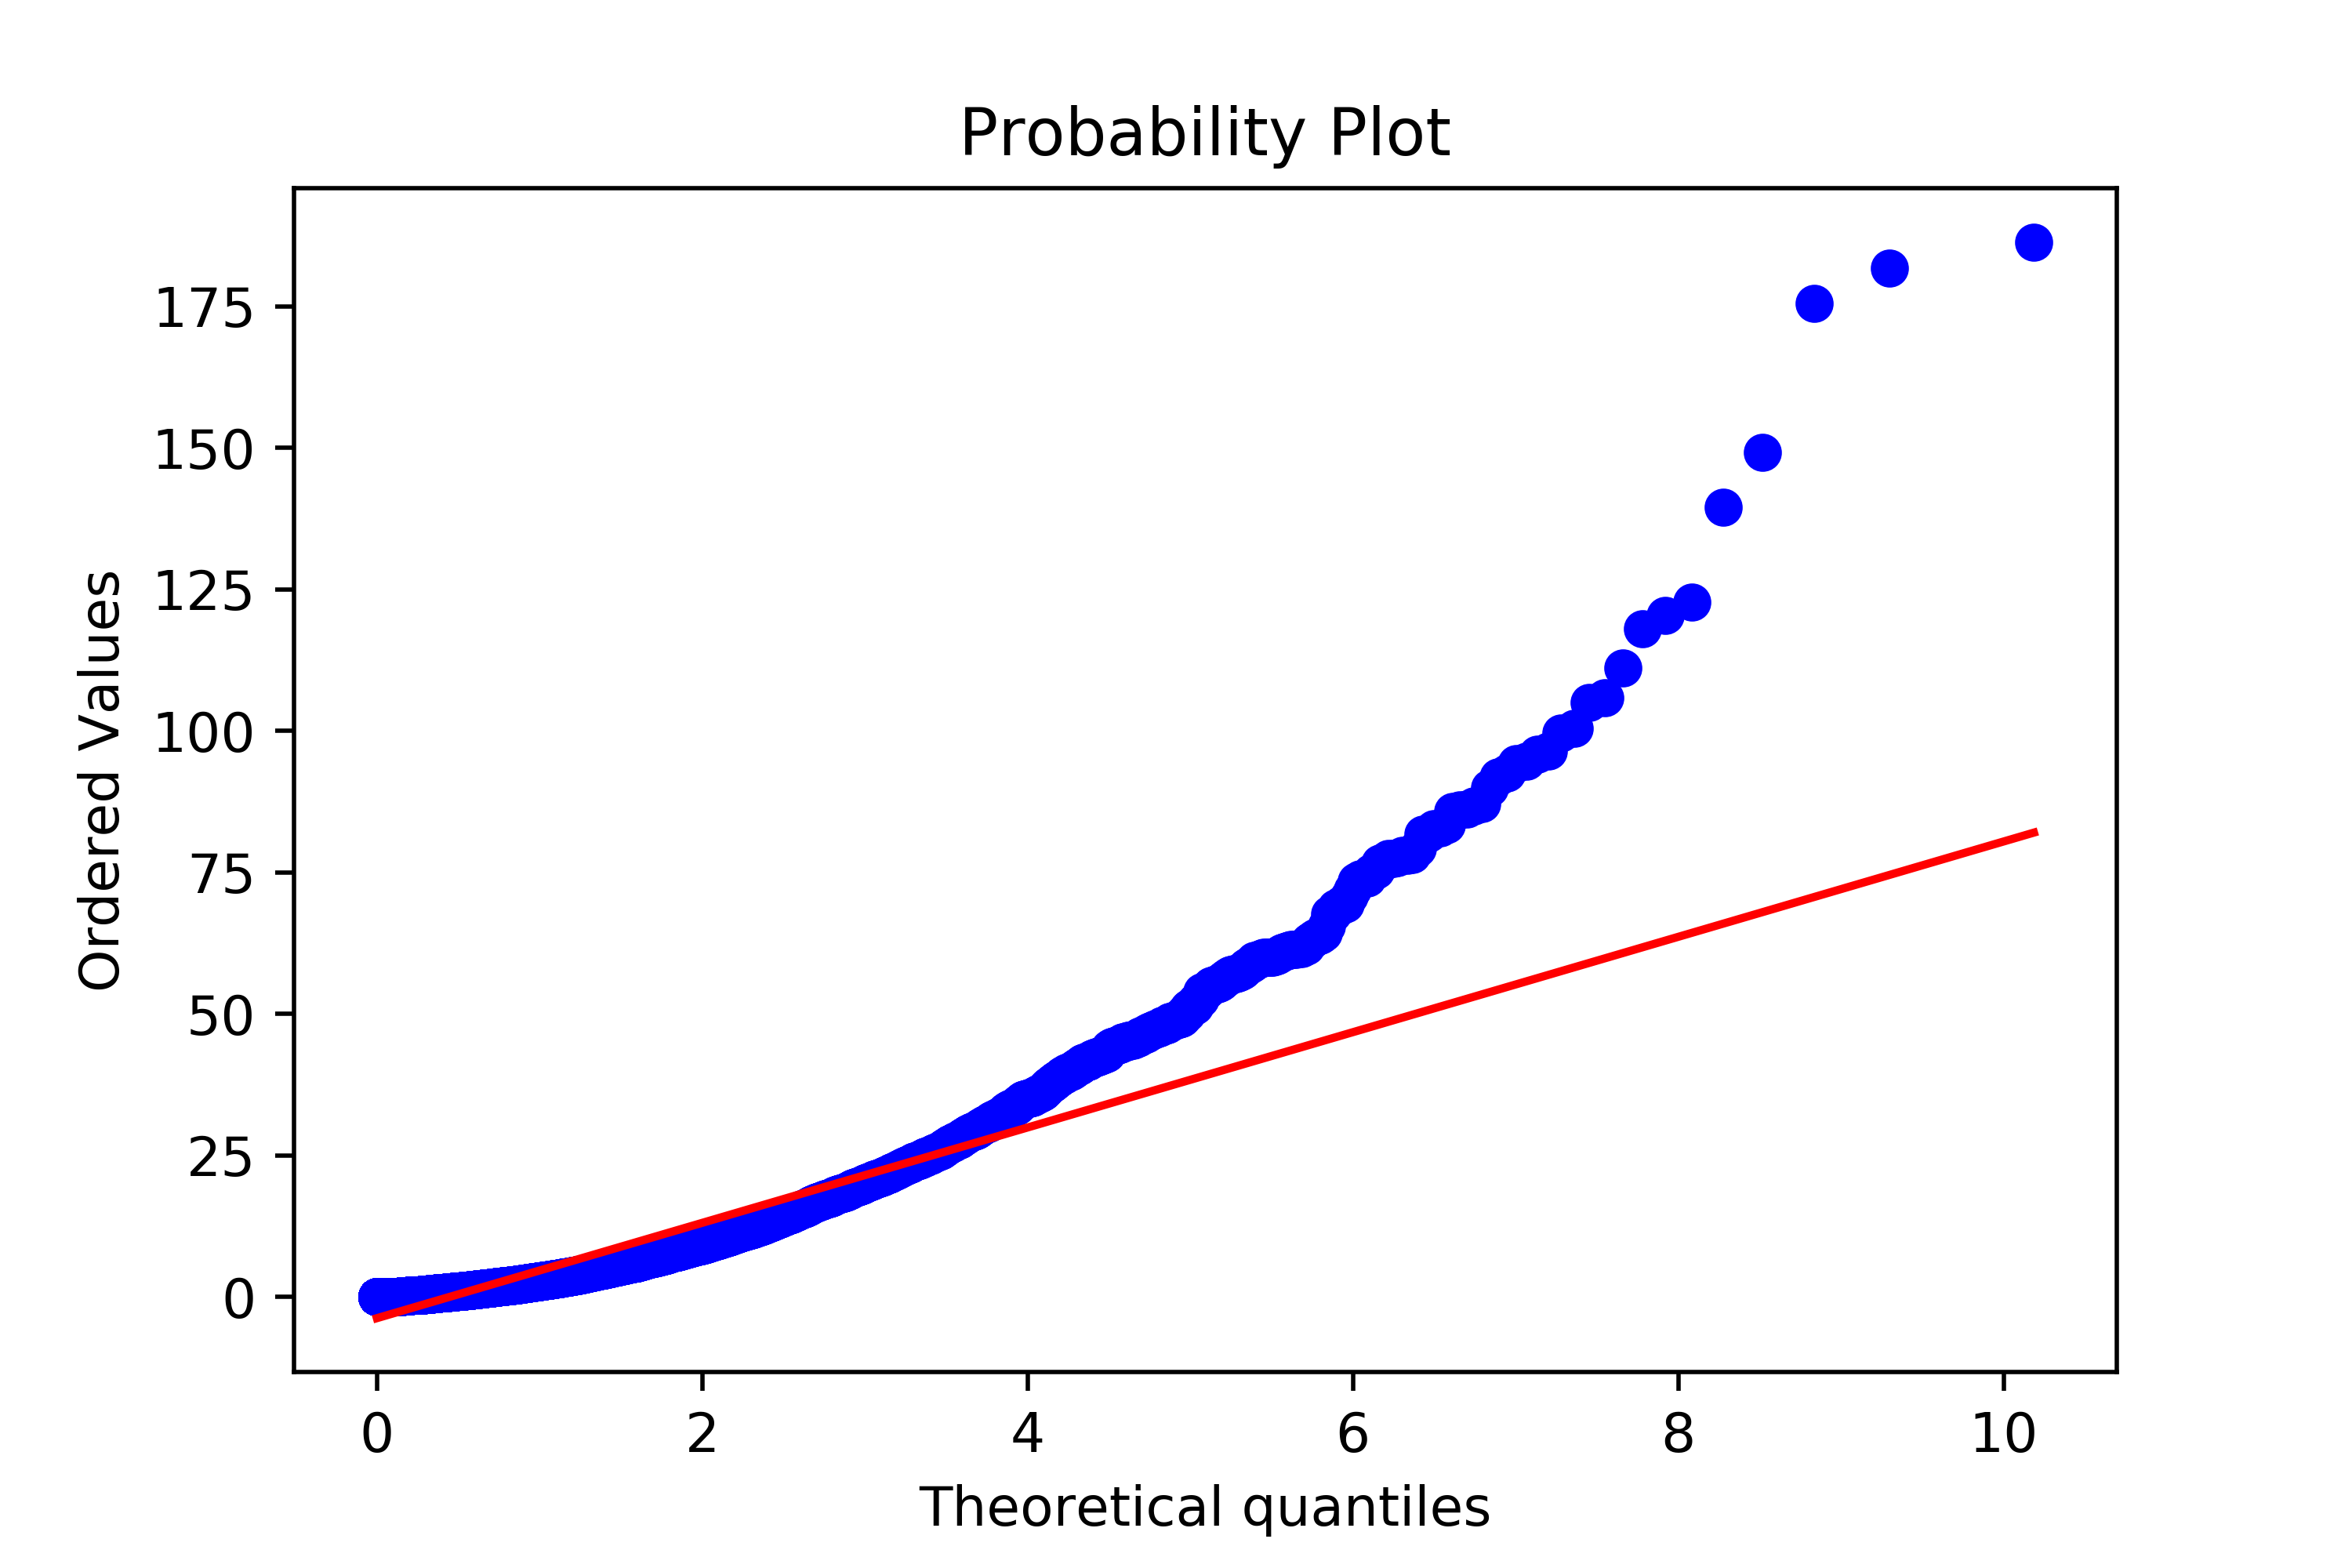
\includegraphics[width=60mm]{Figures/QQ_neg_k1.png}}
{}
&
\subf{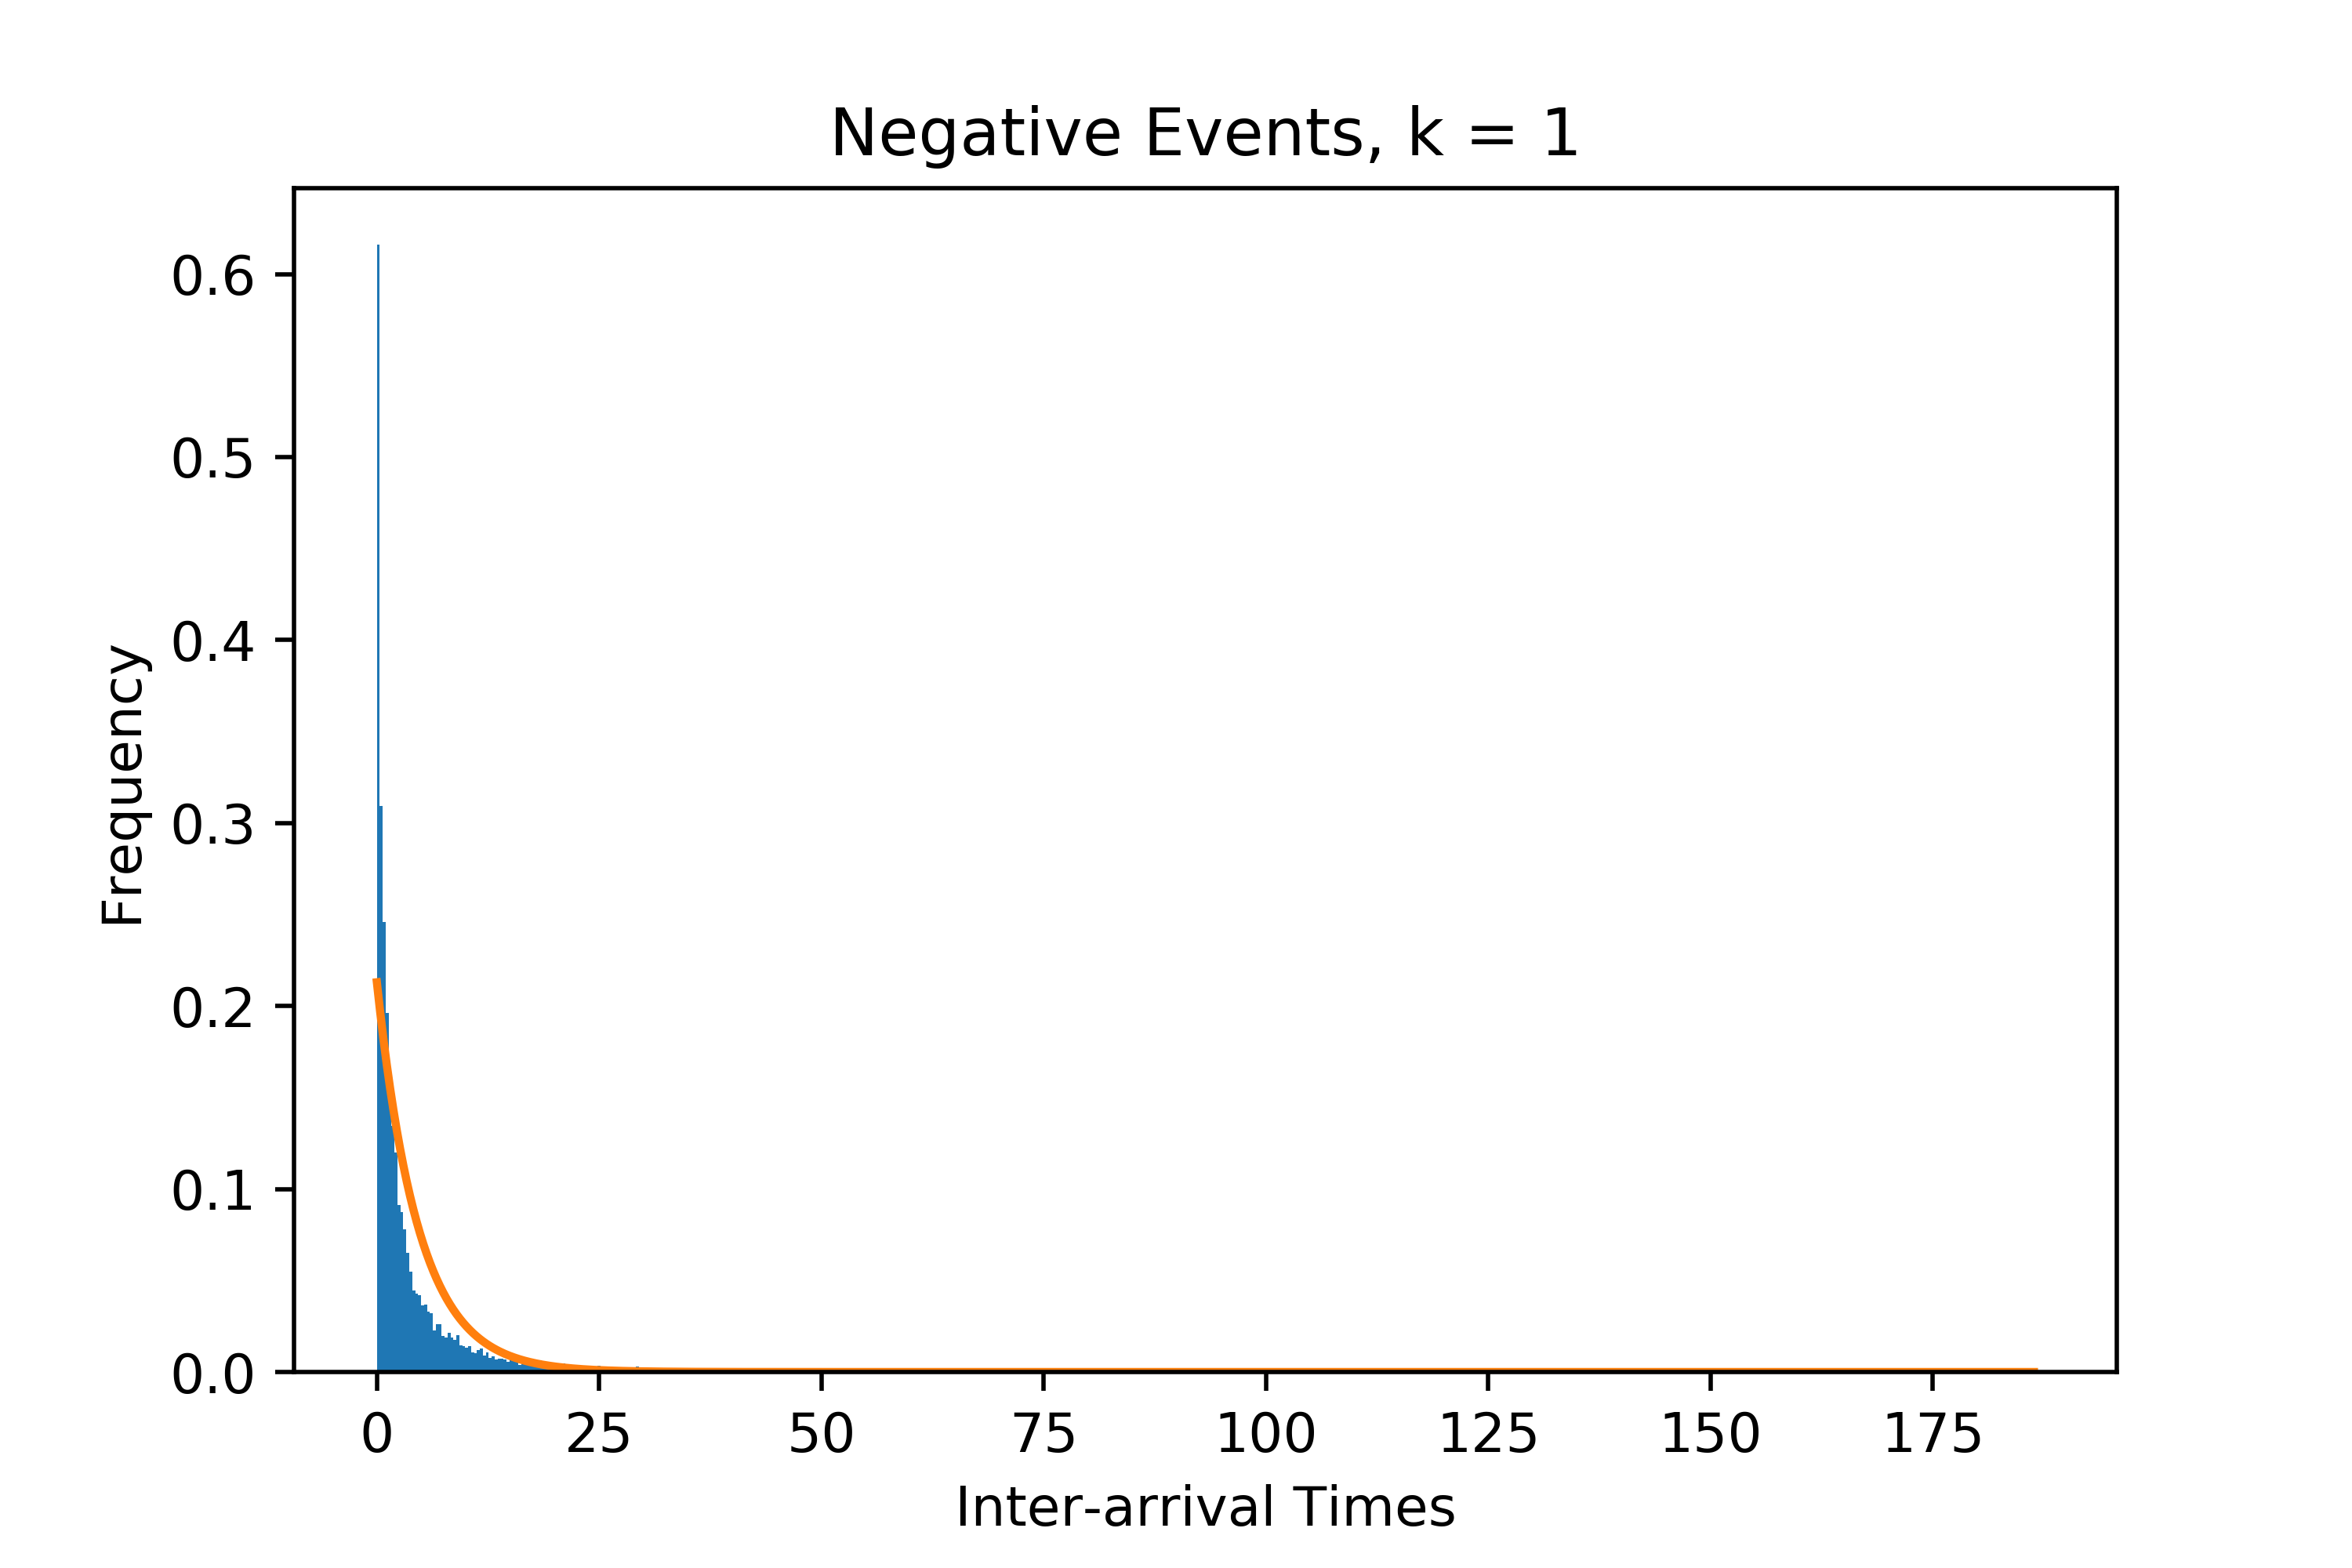
\includegraphics[width=60mm]{Figures/hist_neg_k1.png}}
{}
\\
\subf{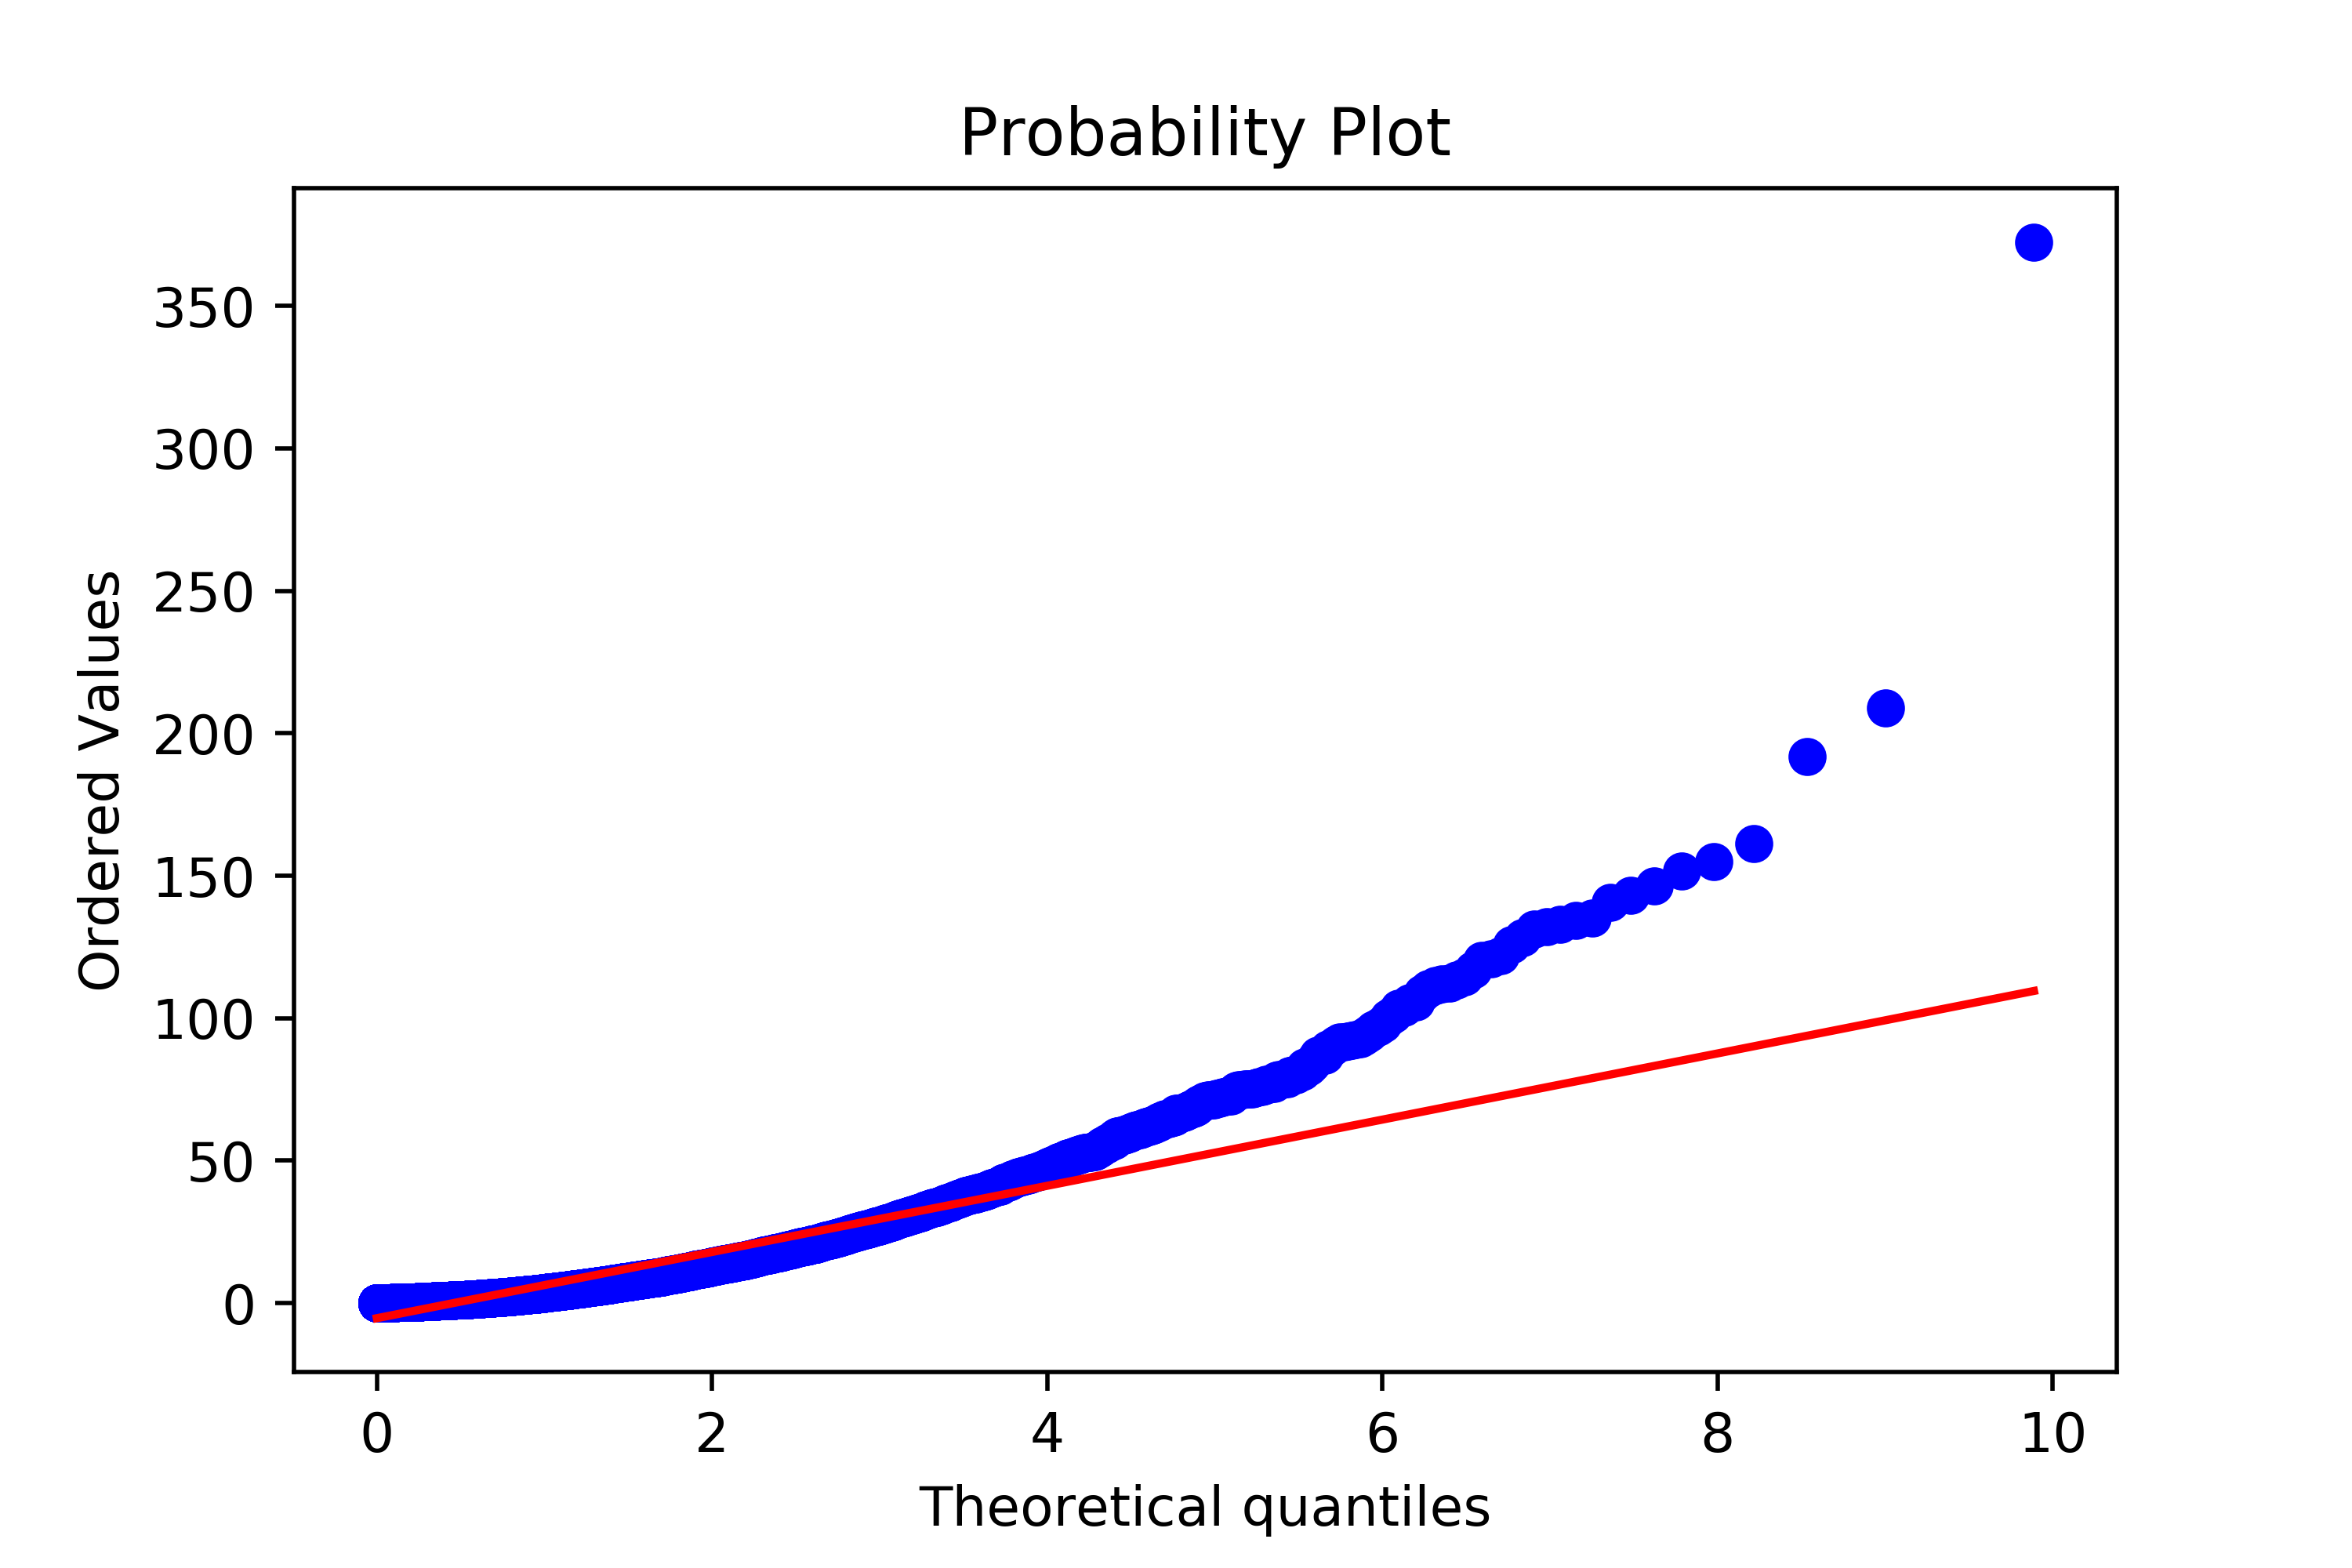
\includegraphics[width=60mm]{Figures/QQ_neg_k2.png}}
{}
&
\subf{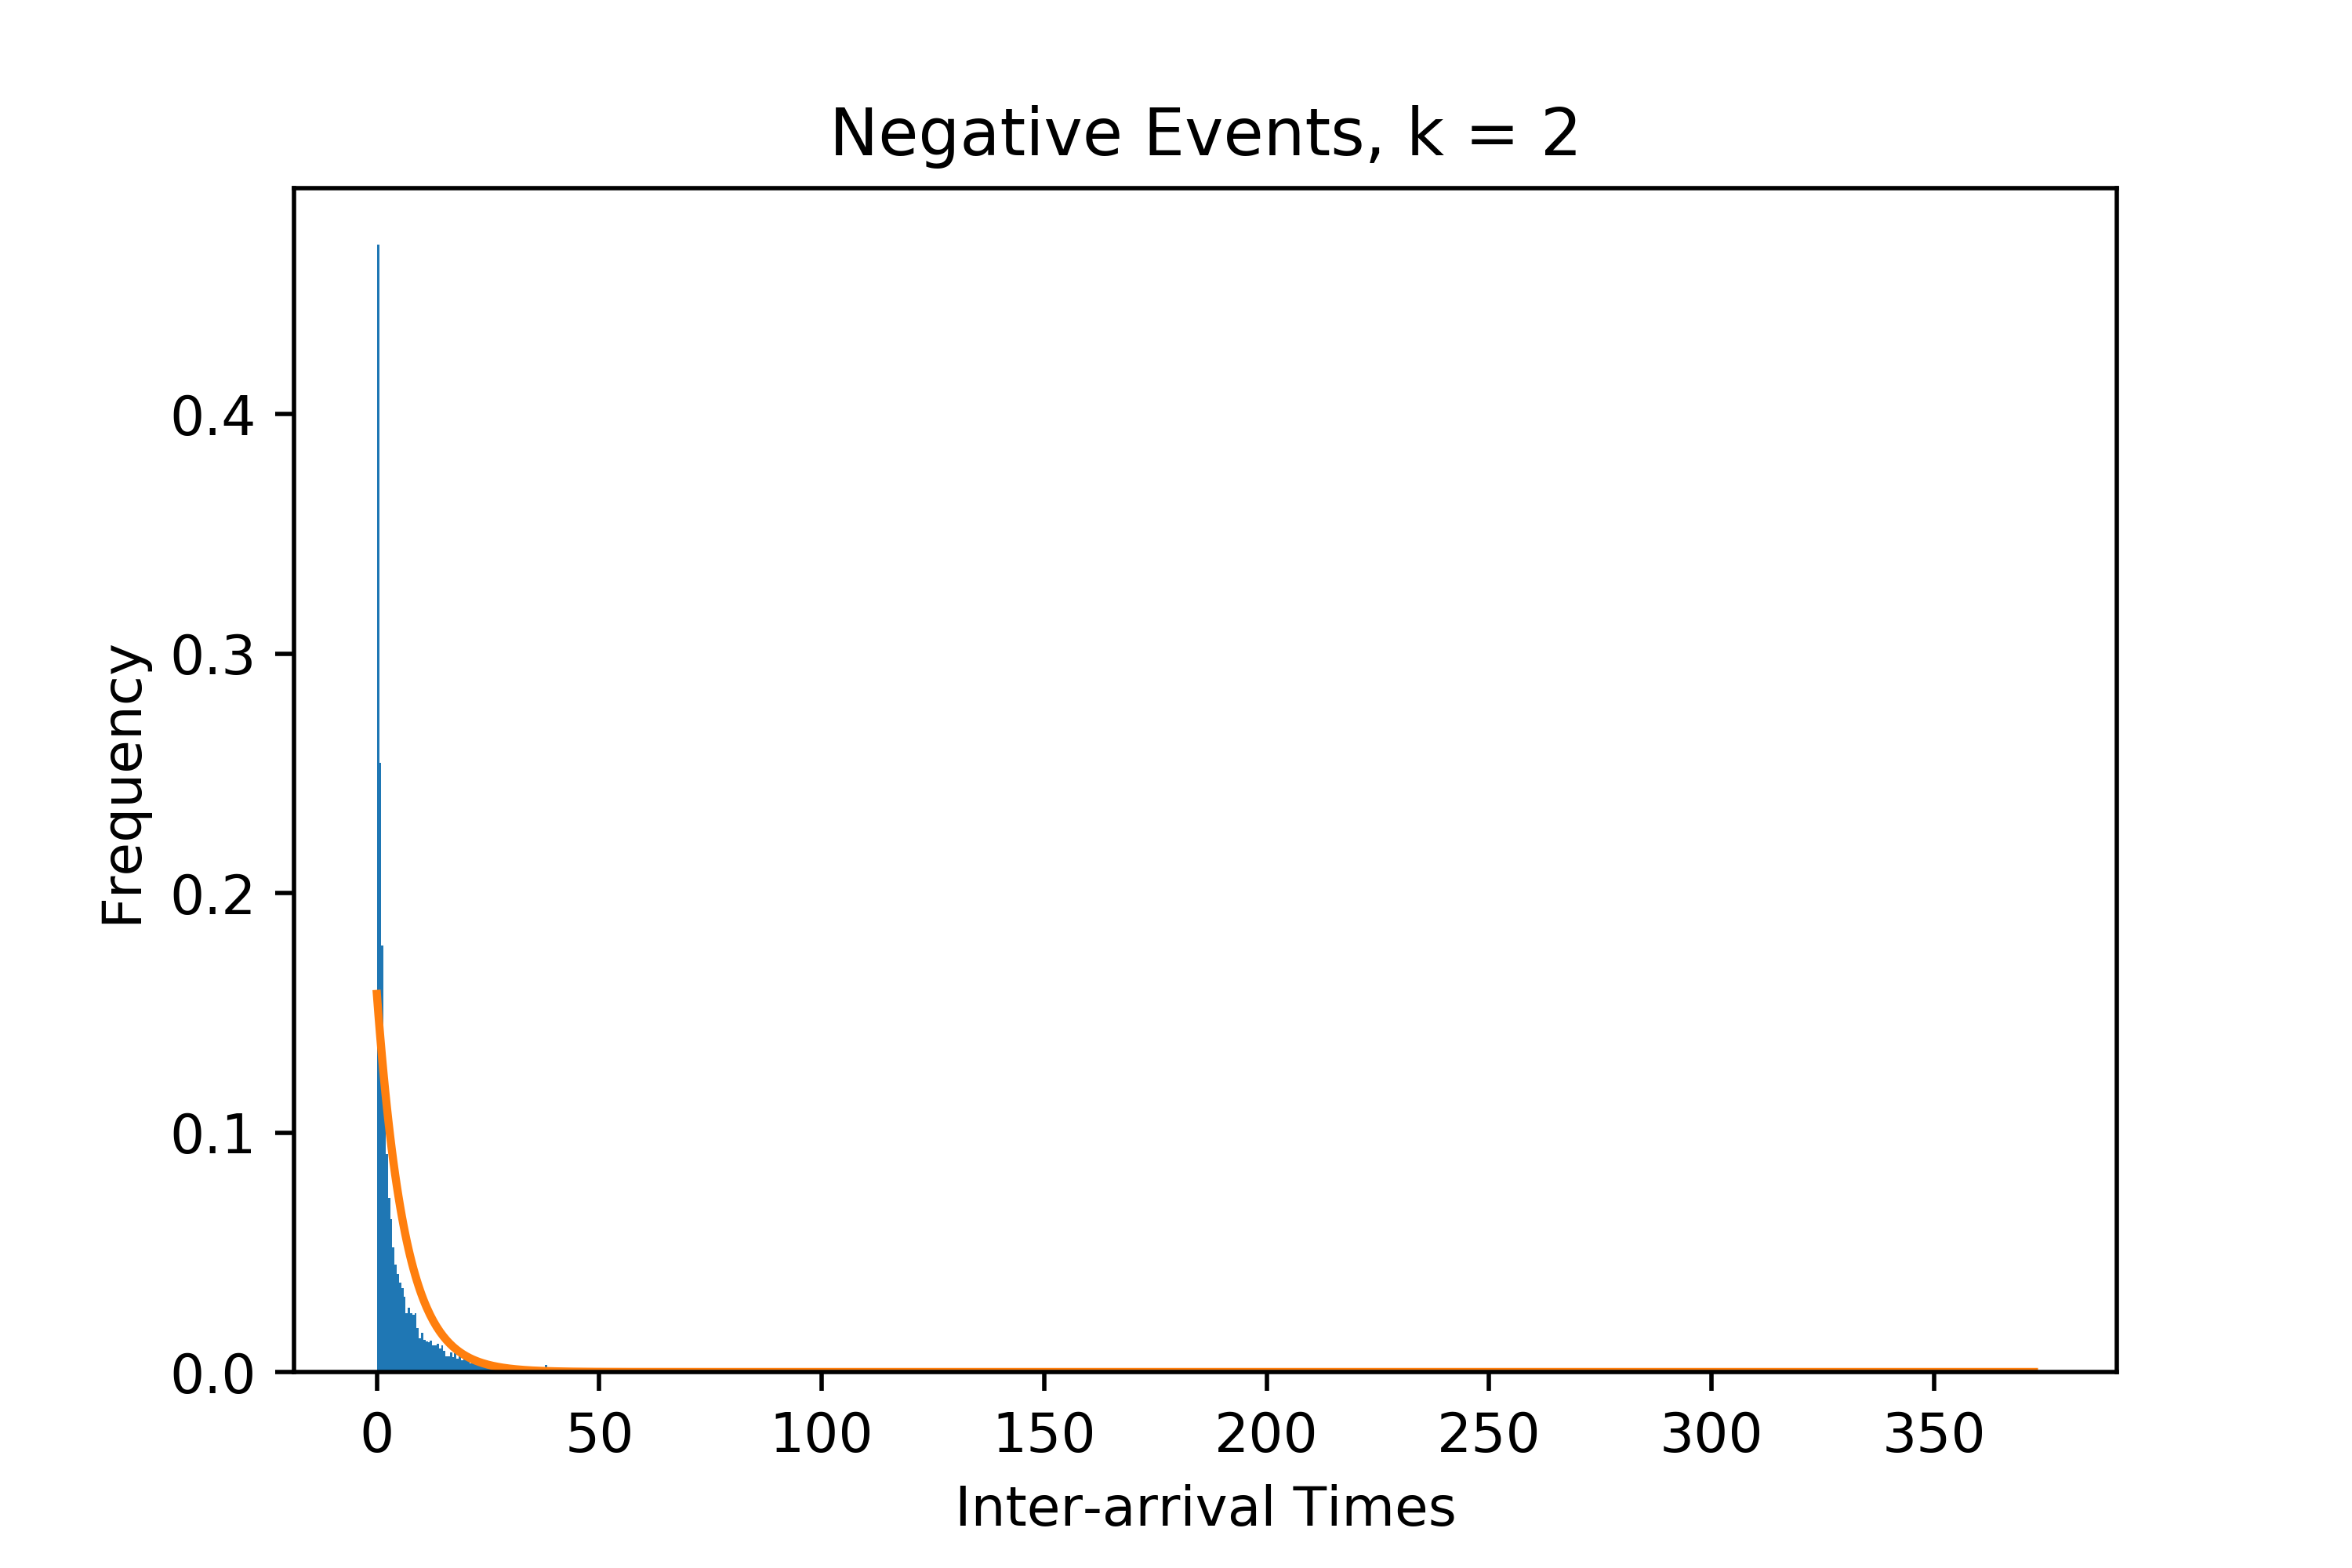
\includegraphics[width=60mm]{Figures/hist_neg_k2.png}}
{}
\\
\hline
\end{tabular}
\label{fig:interarrivals_neg}
\end{figure}

\subsection{Arrival Correlations}\label{ch:correlations}
Although each of the marginal processes can be modelled as a Poisson process, I found that there were significant non-zero correlations between the arrivals at each position. Using a time period $b$ of 60 seconds, I found the correlation between $N^{\pm}_i(b)$ and $N^{\pm}_j(b)$ by sampling random intervals of length $t$ through the period of data collection. The correlation matrix for positive events (closest 8 positions) is shown in Figure \ref{fig:pos_pos_corr} where the entry $(i,j)$ is $corr(N^{+}_i(b), N^{+}_j(b))$. In general, the correlations are positive, with the magnitude of the correlation decreasing as distance from the positions increase.

\begin{figure}[t]
\begin{center}
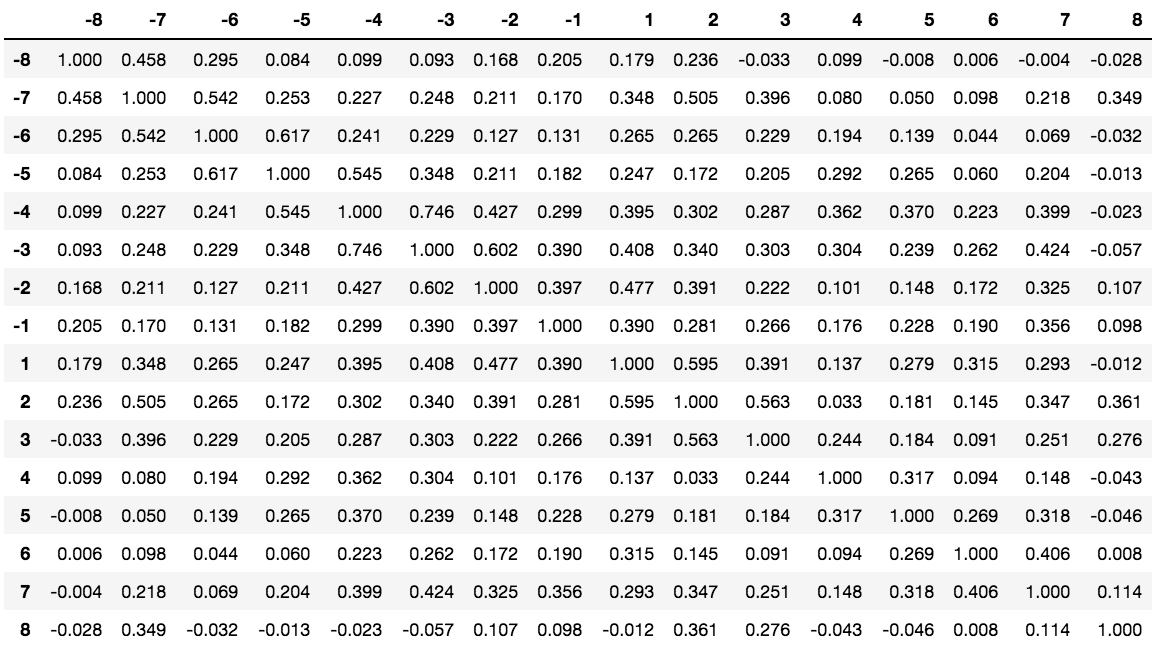
\includegraphics[width=0.8\textwidth]{Figures/pos_pos.png}
\caption{Correlation Matrix for $N^{+}_i(t), N^{+}_j(t)$, $t$ = 60 seconds}
\label{fig:pos_pos_corr}
\end{center}
\end{figure}

The correlation matrix for positive and negative events is shown in Figure \ref{fig:pos_neg_corr} where the entry $(i,j)$ is $corr(N^{+}_i(b), N^{-}_j(b))$. Particularly notable is the very high (nearly 1) correlation between positive and negative at the same position. This could be due to traders reacting to updates by placing orders in the opposite direction, and could indicate that the order book is resilient to changes in the short term.

\begin{figure}[t]
\begin{center}
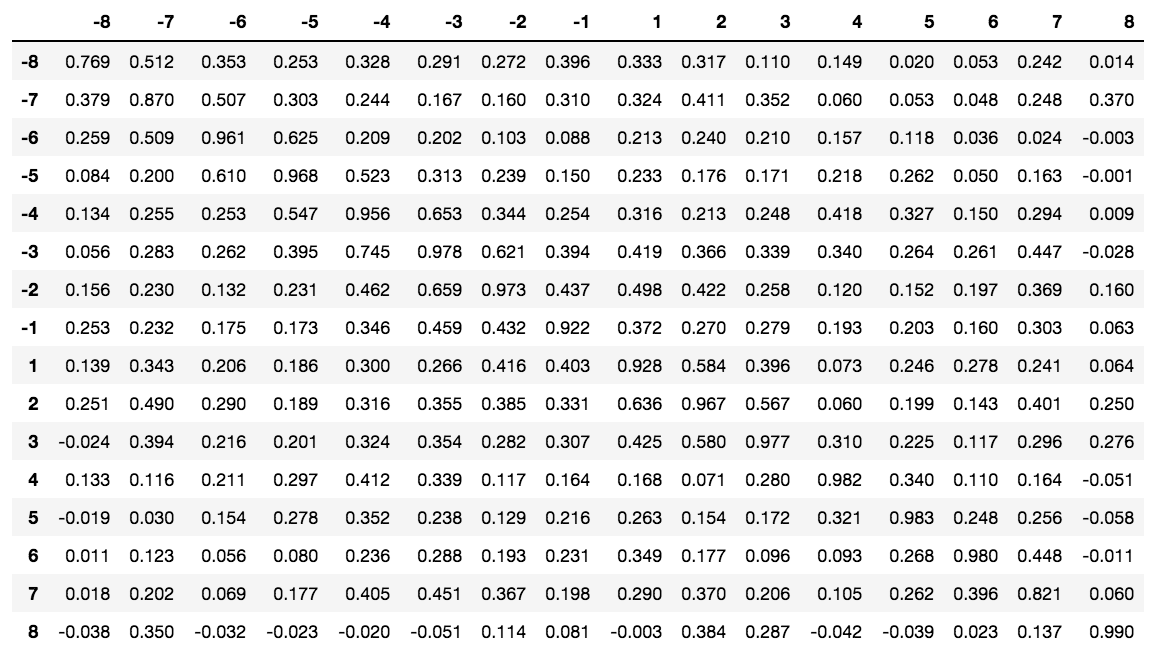
\includegraphics[width=0.8\textwidth]{Figures/pos_neg.png}
\caption{Correlation Matrix for $N^{+}_i(b), N^{-}_j(b)$, $b$ = 60 seconds}
\label{fig:pos_neg_corr}
\end{center}
\end{figure}

The correlation matrix for negative events is shown in Figure \ref{fig:neg_neg_corr} where the entry $(i,j)$ is $corr(N^{-}_i(b), N^{-}_j(b))$. This matrix is similar in nature to the one for positive events. 

\begin{figure}[t]
\begin{center}
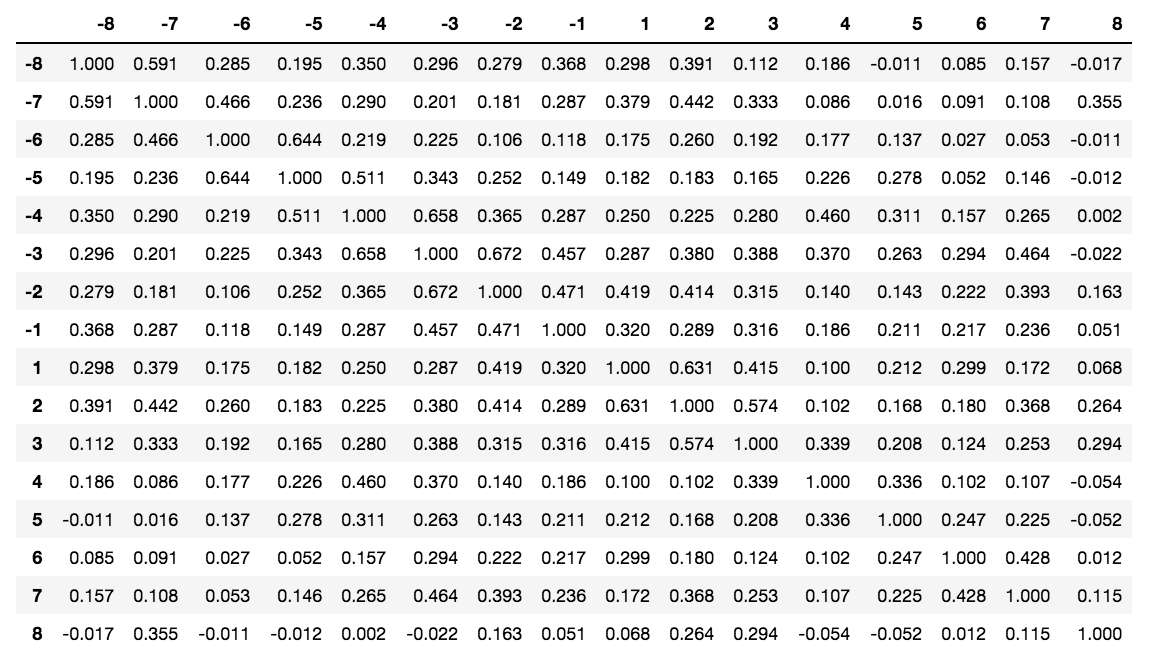
\includegraphics[width=0.8\textwidth]{Figures/neg_neg.png}
\caption{Correlation Matrix for $N^{-}_i(b), N^{-}_j(b)$, $b$ = 60 seconds}
\label{fig:neg_neg_corr}
\end{center}
\end{figure}

These non-zero correlations are clearly non-negligible, so I model the arrivals are a multivariate Poisson process where the arrivals are correlated and each marginal arrival distribution is Poisson. The correlations can be combined to form $\sigma$ as described in subsection \ref{ch:queue_model}. I will discuss the procedure for simulating the multivariate Poisson process in Subsection \ref{ch:simulation_procedure}.

\subsection{Simulation Procedure}\label{ch:simulation_procedure}
In presenting the simulation procedure, it is necessary to discuss the method for generating correlated Poisson processes. I use a method similar to the ones discussed by \cite{A8} to generate multivariate Poisson variables with desired desired correlations. 

The goal is to generate Poisson random variables with means $x_1, x_2, \ldots, x_d$ with means $\lambda_1, \lambda_2, \ldots, \lambda_{d}$ with correlations defined by the matrix $\sigma$. To do so, I make use of a copula. A copula is defined as any joint probability distribution function where each marginal distribution is normally distributed \cite{B1}. That is, 
$$C(u): [0,1]^d \to [0,1]$$ 
is a copula if $C(0, 0, \ldots, 0) = 0$ and $C(1, 1, u_i, 1, \ldots, 1) = u_i$ for all $i$. I will use the Gaussian copula as described in \cite{A8} where

$$ C_\sigma^{Gaussian}(u_1, u_2, \ldots, u_d) = H_\sigma(H^{-1}(u_1), H^{-1}(u_2), \ldots,  H^{-1}(u_d))$$

where $H$ is the inverse cumulative distribution function for a standard random normal variable and $H_\sigma$ is the cumulative distribution function for a random multivariate normal vector with mean $0$ and correlation matrix $R$. I can generate $u$ by first generating a multivariate normal random variable $Y$ with correlation matrix $\sigma$ and setting $(u_1, u_2, \ldots, u_d) = (H^{-1}(u_1), H^{-1}(u_2), \ldots,  H^{-1}(u_d))$. I then pair it with a copula that has marginal Poisson distributions. Namely,

$$ C^{Poisson}(F_1(x_1), F_2(x_2), \ldots, F_d(x_d))$$ where $F_i$ is the discrete cumulative distribution function for a Poisson random variable with rate $\lambda_i$. I can then set

$$(x_1, x_2, \ldots, x_d) = (F^{-1}_1(u_1), F^{-1}_2(u_2), \ldots, F^{-1}_d(u_d))$$

To implement $F^-1_i(u_i)$, I will use the inverse transform method described in \cite{B1}:
\newline

\begin{algorithm}[H]
\SetAlgoLined
\caption{Inverse Transform Method for Poisson Variable With Rate $\lambda$ and input $u$}
 $i = 0$\;
 $p = e^{-\lambda}$\;
 $F = p$\;
 \While{$u >= F$}{
  $p = \lambda p / (i + 1)$ \;
  $F = F + p$ \;
  $i = i + 1$ \;
 }
 return $i$ \;
\end{algorithm}

Each $x_i$ will have marginal have a marginal Poisson distribution with rate $\lambda_i$ and $x$ will approximately have correlation matrix $\sigma$. For code demonstrating the construction of correlated Poisson processes, see listing \ref{correlated-poisson}.

Now, I can simulate arrivals over a time period $T$. I will use backwards-simulation as described in \cite{A7} to simulate arrivals in successive smaller chunks of size $t$. Namely, I will generate $x^+_i$ and $x^-_i$ with means $\lambda^+_i*t$ and $\lambda^-_i*t$ respectively and correlation matrix $\sigma$. Then, I use the fact that conditioned on the number of arrivals in a time period $t$ being equal to $n$, these arrivals are distributed uniformly. 

The simulation algorithm is presented below. I assume that the agent needs to buy $A$ units in a time period $T$ and submits orders of the form $(L,p,v,t)$ which indicates a limit buy order at price $p$ for amount $v$ at time $t$ or $(M,v,t)$ which indicates a market buy order. At the end of the time period, if $A$ units have not been bought, then the trader makes a market order for the remainder of the inventory. I simulate updates in intervals of length $b$.

\begin{algorithm}[H]
\SetAlgoLined
\caption{Simulation of Order Book}
 $n = 0$\;
 Let $L$ be the initial LOB at time $0$. let $L_k$, $k = -K, \ldots, -1, 1, \ldots, K$ be the volumes at each position \;
 Let $a$ be the amount of inventory filled \;
 Let $P$ be the total price \;
 \While{$n*b <= T$ and $a < A$} {
 Let $O$ be the orders submitted by the agent within the interval $[n*b, (n+1)*b)$ \;
 Let $N^+_k, N^-_k$, $k = -K, \ldots, -1, 1, \ldots, K$ be the number of positive and negative arrivals at position $k$. Simulate these values using the procedure described in the beginning of the subsection \;
 For each $k$, generate $N^+_k$ uniform random variables $U \in [0,1)$. The positive updates at position $i$ then occur at times $n*b + b*U$. Do the same for negative arrivals \;
 Take each update and order sorted by time. Treat each of the agent's order as an arrival. A market order or limit order above the best ask is executed immediately at the best price. A limit order is added to the list of active limit orders. Process updates as described in subsection \ref{ch:queue_model}. If a market order or active limit order is filled (must be from market order on the best bid price and taking into account the time priority policy), record the price and volume at which the order is executed and set $a \leftarrow a + v$, $P \leftarrow P + p$ \;
 $ n = n + 1$ \;
 }
 Execute a market order to buy the remaining $A-a$ shares \;
 Return $P$ \;
\end{algorithm}

